\documentclass[11pt]{article}

    \usepackage[breakable]{tcolorbox}
    \usepackage{parskip} % Stop auto-indenting (to mimic markdown behaviour)
    
    \usepackage{iftex}
    \ifPDFTeX
    	\usepackage[T1]{fontenc}
    	\usepackage{mathpazo}
    \else
    	\usepackage{fontspec}
    \fi

    % Basic figure setup, for now with no caption control since it's done
    % automatically by Pandoc (which extracts ![](path) syntax from Markdown).
    \usepackage{graphicx}
    % Maintain compatibility with old templates. Remove in nbconvert 6.0
    \let\Oldincludegraphics\includegraphics
    % Ensure that by default, figures have no caption (until we provide a
    % proper Figure object with a Caption API and a way to capture that
    % in the conversion process - todo).
    \usepackage{caption}
    \DeclareCaptionFormat{nocaption}{}
    \captionsetup{format=nocaption,aboveskip=0pt,belowskip=0pt}

    \usepackage[Export]{adjustbox} % Used to constrain images to a maximum size
    \adjustboxset{max size={0.9\linewidth}{0.9\paperheight}}
    \usepackage{float}
    \floatplacement{figure}{H} % forces figures to be placed at the correct location
    \usepackage{xcolor} % Allow colors to be defined
    \usepackage{enumerate} % Needed for markdown enumerations to work
    \usepackage{geometry} % Used to adjust the document margins
    \usepackage{amsmath} % Equations
    \usepackage{amssymb} % Equations
    \usepackage{textcomp} % defines textquotesingle
    % Hack from http://tex.stackexchange.com/a/47451/13684:
    \AtBeginDocument{%
        \def\PYZsq{\textquotesingle}% Upright quotes in Pygmentized code
    }
    \usepackage{upquote} % Upright quotes for verbatim code
    \usepackage{eurosym} % defines \euro
    \usepackage[mathletters]{ucs} % Extended unicode (utf-8) support
    \usepackage{fancyvrb} % verbatim replacement that allows latex
    \usepackage{grffile} % extends the file name processing of package graphics 
                         % to support a larger range
    \makeatletter % fix for grffile with XeLaTeX
    \def\Gread@@xetex#1{%
      \IfFileExists{"\Gin@base".bb}%
      {\Gread@eps{\Gin@base.bb}}%
      {\Gread@@xetex@aux#1}%
    }
    \makeatother

    % The hyperref package gives us a pdf with properly built
    % internal navigation ('pdf bookmarks' for the table of contents,
    % internal cross-reference links, web links for URLs, etc.)
    \usepackage{hyperref}
    % The default LaTeX title has an obnoxious amount of whitespace. By default,
    % titling removes some of it. It also provides customization options.
    \usepackage{titling}
    \usepackage{longtable} % longtable support required by pandoc >1.10
    \usepackage{booktabs}  % table support for pandoc > 1.12.2
    \usepackage[inline]{enumitem} % IRkernel/repr support (it uses the enumerate* environment)
    \usepackage[normalem]{ulem} % ulem is needed to support strikethroughs (\sout)
                                % normalem makes italics be italics, not underlines
    \usepackage{mathrsfs}
    

    
    % Colors for the hyperref package
    \definecolor{urlcolor}{rgb}{0,.145,.698}
    \definecolor{linkcolor}{rgb}{.71,0.21,0.01}
    \definecolor{citecolor}{rgb}{.12,.54,.11}

    % ANSI colors
    \definecolor{ansi-black}{HTML}{3E424D}
    \definecolor{ansi-black-intense}{HTML}{282C36}
    \definecolor{ansi-red}{HTML}{E75C58}
    \definecolor{ansi-red-intense}{HTML}{B22B31}
    \definecolor{ansi-green}{HTML}{00A250}
    \definecolor{ansi-green-intense}{HTML}{007427}
    \definecolor{ansi-yellow}{HTML}{DDB62B}
    \definecolor{ansi-yellow-intense}{HTML}{B27D12}
    \definecolor{ansi-blue}{HTML}{208FFB}
    \definecolor{ansi-blue-intense}{HTML}{0065CA}
    \definecolor{ansi-magenta}{HTML}{D160C4}
    \definecolor{ansi-magenta-intense}{HTML}{A03196}
    \definecolor{ansi-cyan}{HTML}{60C6C8}
    \definecolor{ansi-cyan-intense}{HTML}{258F8F}
    \definecolor{ansi-white}{HTML}{C5C1B4}
    \definecolor{ansi-white-intense}{HTML}{A1A6B2}
    \definecolor{ansi-default-inverse-fg}{HTML}{FFFFFF}
    \definecolor{ansi-default-inverse-bg}{HTML}{000000}

    % commands and environments needed by pandoc snippets
    % extracted from the output of `pandoc -s`
    \providecommand{\tightlist}{%
      \setlength{\itemsep}{0pt}\setlength{\parskip}{0pt}}
    \DefineVerbatimEnvironment{Highlighting}{Verbatim}{commandchars=\\\{\}}
    % Add ',fontsize=\small' for more characters per line
    \newenvironment{Shaded}{}{}
    \newcommand{\KeywordTok}[1]{\textcolor[rgb]{0.00,0.44,0.13}{\textbf{{#1}}}}
    \newcommand{\DataTypeTok}[1]{\textcolor[rgb]{0.56,0.13,0.00}{{#1}}}
    \newcommand{\DecValTok}[1]{\textcolor[rgb]{0.25,0.63,0.44}{{#1}}}
    \newcommand{\BaseNTok}[1]{\textcolor[rgb]{0.25,0.63,0.44}{{#1}}}
    \newcommand{\FloatTok}[1]{\textcolor[rgb]{0.25,0.63,0.44}{{#1}}}
    \newcommand{\CharTok}[1]{\textcolor[rgb]{0.25,0.44,0.63}{{#1}}}
    \newcommand{\StringTok}[1]{\textcolor[rgb]{0.25,0.44,0.63}{{#1}}}
    \newcommand{\CommentTok}[1]{\textcolor[rgb]{0.38,0.63,0.69}{\textit{{#1}}}}
    \newcommand{\OtherTok}[1]{\textcolor[rgb]{0.00,0.44,0.13}{{#1}}}
    \newcommand{\AlertTok}[1]{\textcolor[rgb]{1.00,0.00,0.00}{\textbf{{#1}}}}
    \newcommand{\FunctionTok}[1]{\textcolor[rgb]{0.02,0.16,0.49}{{#1}}}
    \newcommand{\RegionMarkerTok}[1]{{#1}}
    \newcommand{\ErrorTok}[1]{\textcolor[rgb]{1.00,0.00,0.00}{\textbf{{#1}}}}
    \newcommand{\NormalTok}[1]{{#1}}
    
    % Additional commands for more recent versions of Pandoc
    \newcommand{\ConstantTok}[1]{\textcolor[rgb]{0.53,0.00,0.00}{{#1}}}
    \newcommand{\SpecialCharTok}[1]{\textcolor[rgb]{0.25,0.44,0.63}{{#1}}}
    \newcommand{\VerbatimStringTok}[1]{\textcolor[rgb]{0.25,0.44,0.63}{{#1}}}
    \newcommand{\SpecialStringTok}[1]{\textcolor[rgb]{0.73,0.40,0.53}{{#1}}}
    \newcommand{\ImportTok}[1]{{#1}}
    \newcommand{\DocumentationTok}[1]{\textcolor[rgb]{0.73,0.13,0.13}{\textit{{#1}}}}
    \newcommand{\AnnotationTok}[1]{\textcolor[rgb]{0.38,0.63,0.69}{\textbf{\textit{{#1}}}}}
    \newcommand{\CommentVarTok}[1]{\textcolor[rgb]{0.38,0.63,0.69}{\textbf{\textit{{#1}}}}}
    \newcommand{\VariableTok}[1]{\textcolor[rgb]{0.10,0.09,0.49}{{#1}}}
    \newcommand{\ControlFlowTok}[1]{\textcolor[rgb]{0.00,0.44,0.13}{\textbf{{#1}}}}
    \newcommand{\OperatorTok}[1]{\textcolor[rgb]{0.40,0.40,0.40}{{#1}}}
    \newcommand{\BuiltInTok}[1]{{#1}}
    \newcommand{\ExtensionTok}[1]{{#1}}
    \newcommand{\PreprocessorTok}[1]{\textcolor[rgb]{0.74,0.48,0.00}{{#1}}}
    \newcommand{\AttributeTok}[1]{\textcolor[rgb]{0.49,0.56,0.16}{{#1}}}
    \newcommand{\InformationTok}[1]{\textcolor[rgb]{0.38,0.63,0.69}{\textbf{\textit{{#1}}}}}
    \newcommand{\WarningTok}[1]{\textcolor[rgb]{0.38,0.63,0.69}{\textbf{\textit{{#1}}}}}
    
    
    % Define a nice break command that doesn't care if a line doesn't already
    % exist.
    \def\br{\hspace*{\fill} \\* }
    % Math Jax compatibility definitions
    \def\gt{>}
    \def\lt{<}
    \let\Oldtex\TeX
    \let\Oldlatex\LaTeX
    \renewcommand{\TeX}{\textrm{\Oldtex}}
    \renewcommand{\LaTeX}{\textrm{\Oldlatex}}
    % Document parameters
    % Document title
    \title{HW3}
    
    
    
    
    
% Pygments definitions
\makeatletter
\def\PY@reset{\let\PY@it=\relax \let\PY@bf=\relax%
    \let\PY@ul=\relax \let\PY@tc=\relax%
    \let\PY@bc=\relax \let\PY@ff=\relax}
\def\PY@tok#1{\csname PY@tok@#1\endcsname}
\def\PY@toks#1+{\ifx\relax#1\empty\else%
    \PY@tok{#1}\expandafter\PY@toks\fi}
\def\PY@do#1{\PY@bc{\PY@tc{\PY@ul{%
    \PY@it{\PY@bf{\PY@ff{#1}}}}}}}
\def\PY#1#2{\PY@reset\PY@toks#1+\relax+\PY@do{#2}}

\expandafter\def\csname PY@tok@gd\endcsname{\def\PY@tc##1{\textcolor[rgb]{0.63,0.00,0.00}{##1}}}
\expandafter\def\csname PY@tok@gu\endcsname{\let\PY@bf=\textbf\def\PY@tc##1{\textcolor[rgb]{0.50,0.00,0.50}{##1}}}
\expandafter\def\csname PY@tok@gt\endcsname{\def\PY@tc##1{\textcolor[rgb]{0.00,0.27,0.87}{##1}}}
\expandafter\def\csname PY@tok@gs\endcsname{\let\PY@bf=\textbf}
\expandafter\def\csname PY@tok@gr\endcsname{\def\PY@tc##1{\textcolor[rgb]{1.00,0.00,0.00}{##1}}}
\expandafter\def\csname PY@tok@cm\endcsname{\let\PY@it=\textit\def\PY@tc##1{\textcolor[rgb]{0.25,0.50,0.50}{##1}}}
\expandafter\def\csname PY@tok@vg\endcsname{\def\PY@tc##1{\textcolor[rgb]{0.10,0.09,0.49}{##1}}}
\expandafter\def\csname PY@tok@vi\endcsname{\def\PY@tc##1{\textcolor[rgb]{0.10,0.09,0.49}{##1}}}
\expandafter\def\csname PY@tok@vm\endcsname{\def\PY@tc##1{\textcolor[rgb]{0.10,0.09,0.49}{##1}}}
\expandafter\def\csname PY@tok@mh\endcsname{\def\PY@tc##1{\textcolor[rgb]{0.40,0.40,0.40}{##1}}}
\expandafter\def\csname PY@tok@cs\endcsname{\let\PY@it=\textit\def\PY@tc##1{\textcolor[rgb]{0.25,0.50,0.50}{##1}}}
\expandafter\def\csname PY@tok@ge\endcsname{\let\PY@it=\textit}
\expandafter\def\csname PY@tok@vc\endcsname{\def\PY@tc##1{\textcolor[rgb]{0.10,0.09,0.49}{##1}}}
\expandafter\def\csname PY@tok@il\endcsname{\def\PY@tc##1{\textcolor[rgb]{0.40,0.40,0.40}{##1}}}
\expandafter\def\csname PY@tok@go\endcsname{\def\PY@tc##1{\textcolor[rgb]{0.53,0.53,0.53}{##1}}}
\expandafter\def\csname PY@tok@cp\endcsname{\def\PY@tc##1{\textcolor[rgb]{0.74,0.48,0.00}{##1}}}
\expandafter\def\csname PY@tok@gi\endcsname{\def\PY@tc##1{\textcolor[rgb]{0.00,0.63,0.00}{##1}}}
\expandafter\def\csname PY@tok@gh\endcsname{\let\PY@bf=\textbf\def\PY@tc##1{\textcolor[rgb]{0.00,0.00,0.50}{##1}}}
\expandafter\def\csname PY@tok@ni\endcsname{\let\PY@bf=\textbf\def\PY@tc##1{\textcolor[rgb]{0.60,0.60,0.60}{##1}}}
\expandafter\def\csname PY@tok@nl\endcsname{\def\PY@tc##1{\textcolor[rgb]{0.63,0.63,0.00}{##1}}}
\expandafter\def\csname PY@tok@nn\endcsname{\let\PY@bf=\textbf\def\PY@tc##1{\textcolor[rgb]{0.00,0.00,1.00}{##1}}}
\expandafter\def\csname PY@tok@no\endcsname{\def\PY@tc##1{\textcolor[rgb]{0.53,0.00,0.00}{##1}}}
\expandafter\def\csname PY@tok@na\endcsname{\def\PY@tc##1{\textcolor[rgb]{0.49,0.56,0.16}{##1}}}
\expandafter\def\csname PY@tok@nb\endcsname{\def\PY@tc##1{\textcolor[rgb]{0.00,0.50,0.00}{##1}}}
\expandafter\def\csname PY@tok@nc\endcsname{\let\PY@bf=\textbf\def\PY@tc##1{\textcolor[rgb]{0.00,0.00,1.00}{##1}}}
\expandafter\def\csname PY@tok@nd\endcsname{\def\PY@tc##1{\textcolor[rgb]{0.67,0.13,1.00}{##1}}}
\expandafter\def\csname PY@tok@ne\endcsname{\let\PY@bf=\textbf\def\PY@tc##1{\textcolor[rgb]{0.82,0.25,0.23}{##1}}}
\expandafter\def\csname PY@tok@nf\endcsname{\def\PY@tc##1{\textcolor[rgb]{0.00,0.00,1.00}{##1}}}
\expandafter\def\csname PY@tok@si\endcsname{\let\PY@bf=\textbf\def\PY@tc##1{\textcolor[rgb]{0.73,0.40,0.53}{##1}}}
\expandafter\def\csname PY@tok@s2\endcsname{\def\PY@tc##1{\textcolor[rgb]{0.73,0.13,0.13}{##1}}}
\expandafter\def\csname PY@tok@nt\endcsname{\let\PY@bf=\textbf\def\PY@tc##1{\textcolor[rgb]{0.00,0.50,0.00}{##1}}}
\expandafter\def\csname PY@tok@nv\endcsname{\def\PY@tc##1{\textcolor[rgb]{0.10,0.09,0.49}{##1}}}
\expandafter\def\csname PY@tok@s1\endcsname{\def\PY@tc##1{\textcolor[rgb]{0.73,0.13,0.13}{##1}}}
\expandafter\def\csname PY@tok@dl\endcsname{\def\PY@tc##1{\textcolor[rgb]{0.73,0.13,0.13}{##1}}}
\expandafter\def\csname PY@tok@ch\endcsname{\let\PY@it=\textit\def\PY@tc##1{\textcolor[rgb]{0.25,0.50,0.50}{##1}}}
\expandafter\def\csname PY@tok@m\endcsname{\def\PY@tc##1{\textcolor[rgb]{0.40,0.40,0.40}{##1}}}
\expandafter\def\csname PY@tok@gp\endcsname{\let\PY@bf=\textbf\def\PY@tc##1{\textcolor[rgb]{0.00,0.00,0.50}{##1}}}
\expandafter\def\csname PY@tok@sh\endcsname{\def\PY@tc##1{\textcolor[rgb]{0.73,0.13,0.13}{##1}}}
\expandafter\def\csname PY@tok@ow\endcsname{\let\PY@bf=\textbf\def\PY@tc##1{\textcolor[rgb]{0.67,0.13,1.00}{##1}}}
\expandafter\def\csname PY@tok@sx\endcsname{\def\PY@tc##1{\textcolor[rgb]{0.00,0.50,0.00}{##1}}}
\expandafter\def\csname PY@tok@bp\endcsname{\def\PY@tc##1{\textcolor[rgb]{0.00,0.50,0.00}{##1}}}
\expandafter\def\csname PY@tok@c1\endcsname{\let\PY@it=\textit\def\PY@tc##1{\textcolor[rgb]{0.25,0.50,0.50}{##1}}}
\expandafter\def\csname PY@tok@fm\endcsname{\def\PY@tc##1{\textcolor[rgb]{0.00,0.00,1.00}{##1}}}
\expandafter\def\csname PY@tok@o\endcsname{\def\PY@tc##1{\textcolor[rgb]{0.40,0.40,0.40}{##1}}}
\expandafter\def\csname PY@tok@kc\endcsname{\let\PY@bf=\textbf\def\PY@tc##1{\textcolor[rgb]{0.00,0.50,0.00}{##1}}}
\expandafter\def\csname PY@tok@c\endcsname{\let\PY@it=\textit\def\PY@tc##1{\textcolor[rgb]{0.25,0.50,0.50}{##1}}}
\expandafter\def\csname PY@tok@mf\endcsname{\def\PY@tc##1{\textcolor[rgb]{0.40,0.40,0.40}{##1}}}
\expandafter\def\csname PY@tok@err\endcsname{\def\PY@bc##1{\setlength{\fboxsep}{0pt}\fcolorbox[rgb]{1.00,0.00,0.00}{1,1,1}{\strut ##1}}}
\expandafter\def\csname PY@tok@mb\endcsname{\def\PY@tc##1{\textcolor[rgb]{0.40,0.40,0.40}{##1}}}
\expandafter\def\csname PY@tok@ss\endcsname{\def\PY@tc##1{\textcolor[rgb]{0.10,0.09,0.49}{##1}}}
\expandafter\def\csname PY@tok@sr\endcsname{\def\PY@tc##1{\textcolor[rgb]{0.73,0.40,0.53}{##1}}}
\expandafter\def\csname PY@tok@mo\endcsname{\def\PY@tc##1{\textcolor[rgb]{0.40,0.40,0.40}{##1}}}
\expandafter\def\csname PY@tok@kd\endcsname{\let\PY@bf=\textbf\def\PY@tc##1{\textcolor[rgb]{0.00,0.50,0.00}{##1}}}
\expandafter\def\csname PY@tok@mi\endcsname{\def\PY@tc##1{\textcolor[rgb]{0.40,0.40,0.40}{##1}}}
\expandafter\def\csname PY@tok@kn\endcsname{\let\PY@bf=\textbf\def\PY@tc##1{\textcolor[rgb]{0.00,0.50,0.00}{##1}}}
\expandafter\def\csname PY@tok@cpf\endcsname{\let\PY@it=\textit\def\PY@tc##1{\textcolor[rgb]{0.25,0.50,0.50}{##1}}}
\expandafter\def\csname PY@tok@kr\endcsname{\let\PY@bf=\textbf\def\PY@tc##1{\textcolor[rgb]{0.00,0.50,0.00}{##1}}}
\expandafter\def\csname PY@tok@s\endcsname{\def\PY@tc##1{\textcolor[rgb]{0.73,0.13,0.13}{##1}}}
\expandafter\def\csname PY@tok@kp\endcsname{\def\PY@tc##1{\textcolor[rgb]{0.00,0.50,0.00}{##1}}}
\expandafter\def\csname PY@tok@w\endcsname{\def\PY@tc##1{\textcolor[rgb]{0.73,0.73,0.73}{##1}}}
\expandafter\def\csname PY@tok@kt\endcsname{\def\PY@tc##1{\textcolor[rgb]{0.69,0.00,0.25}{##1}}}
\expandafter\def\csname PY@tok@sc\endcsname{\def\PY@tc##1{\textcolor[rgb]{0.73,0.13,0.13}{##1}}}
\expandafter\def\csname PY@tok@sb\endcsname{\def\PY@tc##1{\textcolor[rgb]{0.73,0.13,0.13}{##1}}}
\expandafter\def\csname PY@tok@sa\endcsname{\def\PY@tc##1{\textcolor[rgb]{0.73,0.13,0.13}{##1}}}
\expandafter\def\csname PY@tok@k\endcsname{\let\PY@bf=\textbf\def\PY@tc##1{\textcolor[rgb]{0.00,0.50,0.00}{##1}}}
\expandafter\def\csname PY@tok@se\endcsname{\let\PY@bf=\textbf\def\PY@tc##1{\textcolor[rgb]{0.73,0.40,0.13}{##1}}}
\expandafter\def\csname PY@tok@sd\endcsname{\let\PY@it=\textit\def\PY@tc##1{\textcolor[rgb]{0.73,0.13,0.13}{##1}}}

\def\PYZbs{\char`\\}
\def\PYZus{\char`\_}
\def\PYZob{\char`\{}
\def\PYZcb{\char`\}}
\def\PYZca{\char`\^}
\def\PYZam{\char`\&}
\def\PYZlt{\char`\<}
\def\PYZgt{\char`\>}
\def\PYZsh{\char`\#}
\def\PYZpc{\char`\%}
\def\PYZdl{\char`\$}
\def\PYZhy{\char`\-}
\def\PYZsq{\char`\'}
\def\PYZdq{\char`\"}
\def\PYZti{\char`\~}
% for compatibility with earlier versions
\def\PYZat{@}
\def\PYZlb{[}
\def\PYZrb{]}
\makeatother


    % For linebreaks inside Verbatim environment from package fancyvrb. 
    \makeatletter
        \newbox\Wrappedcontinuationbox 
        \newbox\Wrappedvisiblespacebox 
        \newcommand*\Wrappedvisiblespace {\textcolor{red}{\textvisiblespace}} 
        \newcommand*\Wrappedcontinuationsymbol {\textcolor{red}{\llap{\tiny$\m@th\hookrightarrow$}}} 
        \newcommand*\Wrappedcontinuationindent {3ex } 
        \newcommand*\Wrappedafterbreak {\kern\Wrappedcontinuationindent\copy\Wrappedcontinuationbox} 
        % Take advantage of the already applied Pygments mark-up to insert 
        % potential linebreaks for TeX processing. 
        %        {, <, #, %, $, ' and ": go to next line. 
        %        _, }, ^, &, >, - and ~: stay at end of broken line. 
        % Use of \textquotesingle for straight quote. 
        \newcommand*\Wrappedbreaksatspecials {% 
            \def\PYGZus{\discretionary{\char`\_}{\Wrappedafterbreak}{\char`\_}}% 
            \def\PYGZob{\discretionary{}{\Wrappedafterbreak\char`\{}{\char`\{}}% 
            \def\PYGZcb{\discretionary{\char`\}}{\Wrappedafterbreak}{\char`\}}}% 
            \def\PYGZca{\discretionary{\char`\^}{\Wrappedafterbreak}{\char`\^}}% 
            \def\PYGZam{\discretionary{\char`\&}{\Wrappedafterbreak}{\char`\&}}% 
            \def\PYGZlt{\discretionary{}{\Wrappedafterbreak\char`\<}{\char`\<}}% 
            \def\PYGZgt{\discretionary{\char`\>}{\Wrappedafterbreak}{\char`\>}}% 
            \def\PYGZsh{\discretionary{}{\Wrappedafterbreak\char`\#}{\char`\#}}% 
            \def\PYGZpc{\discretionary{}{\Wrappedafterbreak\char`\%}{\char`\%}}% 
            \def\PYGZdl{\discretionary{}{\Wrappedafterbreak\char`\$}{\char`\$}}% 
            \def\PYGZhy{\discretionary{\char`\-}{\Wrappedafterbreak}{\char`\-}}% 
            \def\PYGZsq{\discretionary{}{\Wrappedafterbreak\textquotesingle}{\textquotesingle}}% 
            \def\PYGZdq{\discretionary{}{\Wrappedafterbreak\char`\"}{\char`\"}}% 
            \def\PYGZti{\discretionary{\char`\~}{\Wrappedafterbreak}{\char`\~}}% 
        } 
        % Some characters . , ; ? ! / are not pygmentized. 
        % This macro makes them "active" and they will insert potential linebreaks 
        \newcommand*\Wrappedbreaksatpunct {% 
            \lccode`\~`\.\lowercase{\def~}{\discretionary{\hbox{\char`\.}}{\Wrappedafterbreak}{\hbox{\char`\.}}}% 
            \lccode`\~`\,\lowercase{\def~}{\discretionary{\hbox{\char`\,}}{\Wrappedafterbreak}{\hbox{\char`\,}}}% 
            \lccode`\~`\;\lowercase{\def~}{\discretionary{\hbox{\char`\;}}{\Wrappedafterbreak}{\hbox{\char`\;}}}% 
            \lccode`\~`\:\lowercase{\def~}{\discretionary{\hbox{\char`\:}}{\Wrappedafterbreak}{\hbox{\char`\:}}}% 
            \lccode`\~`\?\lowercase{\def~}{\discretionary{\hbox{\char`\?}}{\Wrappedafterbreak}{\hbox{\char`\?}}}% 
            \lccode`\~`\!\lowercase{\def~}{\discretionary{\hbox{\char`\!}}{\Wrappedafterbreak}{\hbox{\char`\!}}}% 
            \lccode`\~`\/\lowercase{\def~}{\discretionary{\hbox{\char`\/}}{\Wrappedafterbreak}{\hbox{\char`\/}}}% 
            \catcode`\.\active
            \catcode`\,\active 
            \catcode`\;\active
            \catcode`\:\active
            \catcode`\?\active
            \catcode`\!\active
            \catcode`\/\active 
            \lccode`\~`\~ 	
        }
    \makeatother

    \let\OriginalVerbatim=\Verbatim
    \makeatletter
    \renewcommand{\Verbatim}[1][1]{%
        %\parskip\z@skip
        \sbox\Wrappedcontinuationbox {\Wrappedcontinuationsymbol}%
        \sbox\Wrappedvisiblespacebox {\FV@SetupFont\Wrappedvisiblespace}%
        \def\FancyVerbFormatLine ##1{\hsize\linewidth
            \vtop{\raggedright\hyphenpenalty\z@\exhyphenpenalty\z@
                \doublehyphendemerits\z@\finalhyphendemerits\z@
                \strut ##1\strut}%
        }%
        % If the linebreak is at a space, the latter will be displayed as visible
        % space at end of first line, and a continuation symbol starts next line.
        % Stretch/shrink are however usually zero for typewriter font.
        \def\FV@Space {%
            \nobreak\hskip\z@ plus\fontdimen3\font minus\fontdimen4\font
            \discretionary{\copy\Wrappedvisiblespacebox}{\Wrappedafterbreak}
            {\kern\fontdimen2\font}%
        }%
        
        % Allow breaks at special characters using \PYG... macros.
        \Wrappedbreaksatspecials
        % Breaks at punctuation characters . , ; ? ! and / need catcode=\active 	
        \OriginalVerbatim[#1,codes*=\Wrappedbreaksatpunct]%
    }
    \makeatother

    % Exact colors from NB
    \definecolor{incolor}{HTML}{303F9F}
    \definecolor{outcolor}{HTML}{D84315}
    \definecolor{cellborder}{HTML}{CFCFCF}
    \definecolor{cellbackground}{HTML}{F7F7F7}
    
    % prompt
    \makeatletter
    \newcommand{\boxspacing}{\kern\kvtcb@left@rule\kern\kvtcb@boxsep}
    \makeatother
    \newcommand{\prompt}[4]{
        \ttfamily\llap{{\color{#2}[#3]:\hspace{3pt}#4}}\vspace{-\baselineskip}
    }
    

    
    % Prevent overflowing lines due to hard-to-break entities
    \sloppy 
    % Setup hyperref package
    \hypersetup{
      breaklinks=true,  % so long urls are correctly broken across lines
      colorlinks=true,
      urlcolor=urlcolor,
      linkcolor=linkcolor,
      citecolor=citecolor,
      }
    % Slightly bigger margins than the latex defaults
    
    \geometry{verbose,tmargin=1in,bmargin=1in,lmargin=1in,rmargin=1in}
    
    

\begin{document}
    
    \maketitle
    
    

    
    \hypertarget{cse-252a-computer-vision-i-fall-2019---homework-3}{%
\section{CSE 252A Computer Vision I Fall 2019 - Homework
3}\label{cse-252a-computer-vision-i-fall-2019---homework-3}}

\hypertarget{instructor-ben-ochoa}{%
\subsection{Instructor: Ben Ochoa}\label{instructor-ben-ochoa}}

\hypertarget{assignment-published-on-tuesday-october-22-2019}{%
\subsubsection{Assignment published on: Tuesday, October 22,
2019}\label{assignment-published-on-tuesday-october-22-2019}}

\hypertarget{due-on-tuesday-november-5-2019-1159-pm}{%
\subsubsection{Due on: Tuesday, November 5, 2019 11:59
pm}\label{due-on-tuesday-november-5-2019-1159-pm}}

\hypertarget{instructions}{%
\subsection{Instructions}\label{instructions}}

\begin{itemize}
\tightlist
\item
  Review the academic integrity and collaboration policies on the course
  website.

  \begin{itemize}
  \tightlist
  \item
    This assignment must be completed individually.
  \end{itemize}
\item
  All solutions must be written in this notebook.

  \begin{itemize}
  \tightlist
  \item
    This includes the theoretical problems, for which you \textbf{must}
    write your answers in Markdown cells (using LaTeX when appropriate).
  \item
    Programming aspects of the assignment must be completed using Python
    in this notebook.
  \end{itemize}
\item
  If you want to modify the skeleton code, you may do so. It has only
  been provided as a framework for your solution.
\item
  You may use Python packages (such as NumPy and SciPy) for basic linear
  algebra, but you may not use packages that directly solve the problem.

  \begin{itemize}
  \tightlist
  \item
    If you are unsure about using a specific package or function, then
    ask the instructor and/or teaching assistants for clarification.
  \end{itemize}
\item
  You must submit this notebook exported as a PDF. You must also submit
  this notebook as \texttt{.ipynb} file.

  \begin{itemize}
  \tightlist
  \item
    Submit both files (\texttt{.pdf} and \texttt{.ipynb}) on Gradescope.
  \item
    \textbf{You must mark the PDF pages associated with each question in
    Gradescope. If you fail to do so, we may dock points.}
  \end{itemize}
\item
  It is highly recommended that you begin working on this assignment
  early.
\item
  \textbf{Late policy: assignments submitted late will receive a 15\%
  grade reduction for each 12 hours late (i.e., 30\% per day).
  Assignments will not be accepted 72 hours after the due date. If you
  require an extension (for personal reasons only) to a due date, you
  must request one as far in advance as possible. Extensions requested
  close to or after the due date will only be granted for clear
  emergencies or clearly unforeseeable circumstances.}
\end{itemize}

    \hypertarget{problem-1-photometric-stereo-specularity-removal-20-pts}{%
\subsection{Problem 1: Photometric Stereo, Specularity Removal {[}20
pts{]}}\label{problem-1-photometric-stereo-specularity-removal-20-pts}}

The goal of this problem is to implement a couple of different
algorithms that reconstruct a surface using the concept of Lambertian
photometric stereo. Additionally, you will implement the specular
removal technique of
\href{http://www.eecs.harvard.edu/~zickler/download/photodiff_cvpr05_preprint.pdf}{Mallick
et al.}, which enables photometric stereo to be performed on certain
non-Lambertian materials.

You can assume a Lambertian reflectance function once specularities are
removed. However, note that the albedo is unknown and non-constant in
the images you will use.

As input, your program should take in multiple images along with the
light source direction for each image. Each image is associated with
only a single light, and hence a single direction.

\hypertarget{data}{%
\subsubsection{Data}\label{data}}

You will use synthetic images and specular sphere images as data. These
images are stored in \texttt{.pickle} files which have been graciously
provided by Satya Mallick. Each \texttt{.pickle} file contains

\begin{itemize}
\tightlist
\item
  \texttt{im1}, \texttt{im2}, \texttt{im3}, \texttt{im4}, \ldots{}
  images.
\item
  \texttt{l1}, \texttt{l2}, \texttt{l3}, \texttt{l4}, \ldots{} light
  source directions.
\end{itemize}

    \hypertarget{part-1-lambertian-photometric-stereo-8-pts}{%
\subsubsection{Part 1: Lambertian Photometric Stereo {[}8
pts{]}}\label{part-1-lambertian-photometric-stereo-8-pts}}

Implement the photometric stereo technique described in the lecture
slides and in Forsyth and Ponce 2.2.4 (\emph{Photometric Stereo: Shape
from Multiple Shaded Images}). Your program should have two parts:

\begin{enumerate}
\def\labelenumi{\arabic{enumi}.}
\item
  Read in the images and corresponding light source directions, and
  estimate the surface normals and albedo map.
\item
  Reconstruct the depth map from the surface normals. You should first
  try the naive scanline-based ``shape by integration'' method described
  in the book and in lecture. (You are required to implement this.) For
  comparison, you should also integrate using the Horn technique which
  is already implemented for you in the \texttt{horn\_integrate}
  function. Note that for good results you will often want to run the
  \texttt{horn\_integrate} function with 10000-100000 iterations, which
  will take a while. For your final submission, we will require that you
  run Horn integration for 1000 (one thousand) iterations or more in
  each case. But for debugging, it is suggested that you keep the number
  of iterations low.
\end{enumerate}

You will find all the data for this part in
\texttt{synthetic\_data.pickle}. Try using only \texttt{im1},
\texttt{im2} and \texttt{im4} first. Display your outputs as mentioned
below.

Then use all four images (most accurate).

For \textbf{each} of the \textbf{two above cases} you must output:

\begin{enumerate}
\def\labelenumi{\arabic{enumi}.}
\item
  The estimated albedo map.
\item
  The estimated surface normals by showing both

  \begin{enumerate}
  \def\labelenumii{\arabic{enumii}.}
  \tightlist
  \item
    Needle map, and
  \item
    Three images showing each of the surface normal components.
  \end{enumerate}
\item
  A wireframe of the depth map given by the scanline method.
\item
  A wireframe of the depth map given by Horn integration.
\end{enumerate}

In total, we expect 2 * 7 = 14 images for this part.

An example of outputs is shown in the figure below. (The example outputs
only include one depth map, although we expect two -- see above.)

\begin{figure}
\centering
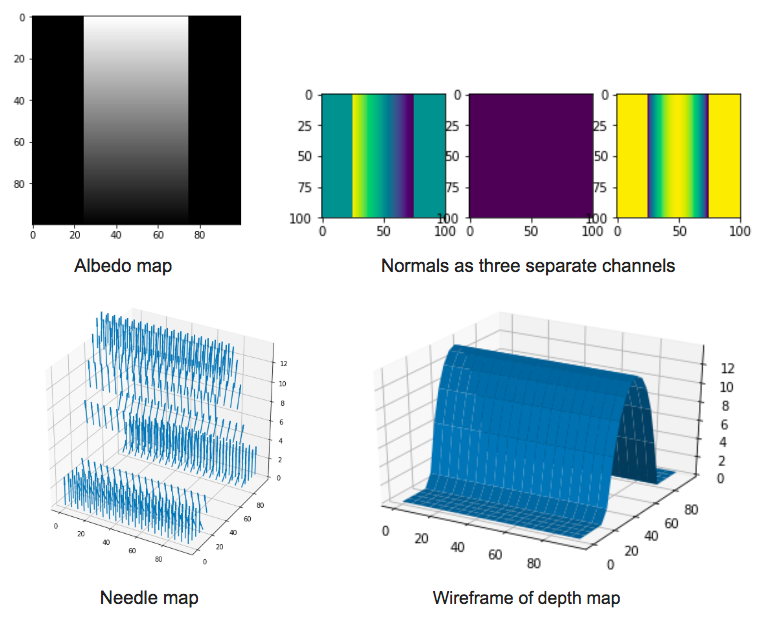
\includegraphics{problem1_example.png}
\caption{Problem 1.1 example outputs}
\end{figure}

    \begin{tcolorbox}[breakable, size=fbox, boxrule=1pt, pad at break*=1mm,colback=cellbackground, colframe=cellborder]
\prompt{In}{incolor}{198}{\boxspacing}
\begin{Verbatim}[commandchars=\\\{\}]
\PY{c+c1}{\PYZsh{} Setup}
\PY{k+kn}{import} \PY{n+nn}{pickle}
\PY{k+kn}{import} \PY{n+nn}{numpy} \PY{k}{as} \PY{n+nn}{np}
\PY{k+kn}{from} \PY{n+nn}{time} \PY{k}{import} \PY{n}{time}
\PY{k+kn}{from} \PY{n+nn}{skimage} \PY{k}{import} \PY{n}{io}
\PY{o}{\PYZpc{}}\PY{k}{matplotlib} inline
\PY{k+kn}{import} \PY{n+nn}{matplotlib}\PY{n+nn}{.}\PY{n+nn}{pyplot} \PY{k}{as} \PY{n+nn}{plt}

\PY{c+c1}{\PYZsh{}\PYZsh{}\PYZsh{} Example: how to read and access data from a .pickle file}
\PY{n}{pickle\PYZus{}in} \PY{o}{=} \PY{n+nb}{open}\PY{p}{(}\PY{l+s+s2}{\PYZdq{}}\PY{l+s+s2}{synthetic\PYZus{}data.pickle}\PY{l+s+s2}{\PYZdq{}}\PY{p}{,} \PY{l+s+s2}{\PYZdq{}}\PY{l+s+s2}{rb}\PY{l+s+s2}{\PYZdq{}}\PY{p}{)}
\PY{n}{data} \PY{o}{=} \PY{n}{pickle}\PY{o}{.}\PY{n}{load}\PY{p}{(}\PY{n}{pickle\PYZus{}in}\PY{p}{,} \PY{n}{encoding}\PY{o}{=}\PY{l+s+s2}{\PYZdq{}}\PY{l+s+s2}{latin1}\PY{l+s+s2}{\PYZdq{}}\PY{p}{)}

\PY{c+c1}{\PYZsh{} data is a dict which stores each element as a key\PYZhy{}value pair. }
\PY{n+nb}{print}\PY{p}{(}\PY{l+s+s2}{\PYZdq{}}\PY{l+s+s2}{Keys: }\PY{l+s+s2}{\PYZdq{}}\PY{p}{,} \PY{n+nb}{list}\PY{p}{(}\PY{n}{data}\PY{o}{.}\PY{n}{keys}\PY{p}{(}\PY{p}{)}\PY{p}{)}\PY{p}{)}

\PY{c+c1}{\PYZsh{} To access the value of an entity, refer to it by its key.}
\PY{k}{for} \PY{n}{i} \PY{o+ow}{in} \PY{n+nb}{range}\PY{p}{(}\PY{l+m+mi}{1}\PY{p}{,} \PY{l+m+mi}{5}\PY{p}{)}\PY{p}{:}
    \PY{n+nb}{print}\PY{p}{(}\PY{l+s+s2}{\PYZdq{}}\PY{l+s+se}{\PYZbs{}n}\PY{l+s+s2}{Image }\PY{l+s+si}{\PYZpc{}d}\PY{l+s+s2}{:}\PY{l+s+s2}{\PYZdq{}} \PY{o}{\PYZpc{}} \PY{n}{i}\PY{p}{)}
    \PY{n}{plt}\PY{o}{.}\PY{n}{imshow}\PY{p}{(}\PY{n}{data}\PY{p}{[}\PY{l+s+s2}{\PYZdq{}}\PY{l+s+s2}{im}\PY{l+s+si}{\PYZpc{}d}\PY{l+s+s2}{\PYZdq{}} \PY{o}{\PYZpc{}} \PY{n}{i}\PY{p}{]}\PY{p}{,} \PY{n}{cmap}\PY{o}{=}\PY{l+s+s2}{\PYZdq{}}\PY{l+s+s2}{gray}\PY{l+s+s2}{\PYZdq{}}\PY{p}{)}
    \PY{n}{plt}\PY{o}{.}\PY{n}{show}\PY{p}{(}\PY{p}{)}
    \PY{n+nb}{print}\PY{p}{(}\PY{l+s+s2}{\PYZdq{}}\PY{l+s+s2}{Light source direction: }\PY{l+s+s2}{\PYZdq{}} \PY{o}{+} \PY{n+nb}{str}\PY{p}{(}\PY{n}{data}\PY{p}{[}\PY{l+s+s2}{\PYZdq{}}\PY{l+s+s2}{l}\PY{l+s+si}{\PYZpc{}d}\PY{l+s+s2}{\PYZdq{}} \PY{o}{\PYZpc{}} \PY{n}{i}\PY{p}{]}\PY{p}{)}\PY{p}{)}
\end{Verbatim}
\end{tcolorbox}

    \begin{Verbatim}[commandchars=\\\{\}]
Keys:  ['\_\_version\_\_', 'l4', '\_\_header\_\_', 'im1', 'im3', 'im2', 'l2', 'im4',
'l1', '\_\_globals\_\_', 'l3']

Image 1:
    \end{Verbatim}

    \begin{center}
    \adjustimage{max size={0.9\linewidth}{0.9\paperheight}}{output_3_1.png}
    \end{center}
    { \hspace*{\fill} \\}
    
    \begin{Verbatim}[commandchars=\\\{\}]
Light source direction: [[0 0 1]]

Image 2:
    \end{Verbatim}

    \begin{center}
    \adjustimage{max size={0.9\linewidth}{0.9\paperheight}}{output_3_3.png}
    \end{center}
    { \hspace*{\fill} \\}
    
    \begin{Verbatim}[commandchars=\\\{\}]
Light source direction: [[0.2 0.  1. ]]

Image 3:
    \end{Verbatim}

    \begin{center}
    \adjustimage{max size={0.9\linewidth}{0.9\paperheight}}{output_3_5.png}
    \end{center}
    { \hspace*{\fill} \\}
    
    \begin{Verbatim}[commandchars=\\\{\}]
Light source direction: [[-0.2  0.   1. ]]

Image 4:
    \end{Verbatim}

    \begin{center}
    \adjustimage{max size={0.9\linewidth}{0.9\paperheight}}{output_3_7.png}
    \end{center}
    { \hspace*{\fill} \\}
    
    \begin{Verbatim}[commandchars=\\\{\}]
Light source direction: [[0.  0.2 1. ]]
    \end{Verbatim}

    Based on the above images, can you interpret the orientation of the
coordinate frame? If we label the axes in order as x, y, z, then the
x-axis points left, the y-axis points up, and the z-axis points out of
the screen in our direction. (That means this is a left-handed
coordinate system. How will this affect the scanline integration
algorithm? Hint: if you integrate rightward along the x-axis and
downward along the y-axis, you will be doing in opposite directions to
the axes, and the partial derivatives you compute may need to be
modified.)

\emph{Note: as clarification, no direct response is needed for this
cell.}

    \begin{tcolorbox}[breakable, size=fbox, boxrule=1pt, pad at break*=1mm,colback=cellbackground, colframe=cellborder]
\prompt{In}{incolor}{244}{\boxspacing}
\begin{Verbatim}[commandchars=\\\{\}]
\PY{k+kn}{import} \PY{n+nn}{numpy} \PY{k}{as} \PY{n+nn}{np}
\PY{k+kn}{from} \PY{n+nn}{scipy}\PY{n+nn}{.}\PY{n+nn}{signal} \PY{k}{import} \PY{n}{convolve}

\PY{k}{def} \PY{n+nf}{horn\PYZus{}integrate}\PY{p}{(}\PY{n}{gx}\PY{p}{,} \PY{n}{gy}\PY{p}{,} \PY{n}{mask}\PY{p}{,} \PY{n}{niter}\PY{p}{)}\PY{p}{:}
    \PY{l+s+sd}{\PYZdq{}\PYZdq{}\PYZdq{}}
\PY{l+s+sd}{    horn\PYZus{}integrate recovers the function g from its partial }
\PY{l+s+sd}{    derivatives gx and gy. }
\PY{l+s+sd}{    mask is a binary image which tells which pixels are }
\PY{l+s+sd}{    involved in integration. }
\PY{l+s+sd}{    niter is the number of iterations. }
\PY{l+s+sd}{    typically 100,000 or 200,000, }
\PY{l+s+sd}{    although the trend can be seen even after 1000 iterations.}
\PY{l+s+sd}{    \PYZdq{}\PYZdq{}\PYZdq{}}
    \PY{n}{g} \PY{o}{=} \PY{n}{np}\PY{o}{.}\PY{n}{ones}\PY{p}{(}\PY{n}{np}\PY{o}{.}\PY{n}{shape}\PY{p}{(}\PY{n}{gx}\PY{p}{)}\PY{p}{)}
    
    \PY{n}{gx} \PY{o}{=} \PY{n}{np}\PY{o}{.}\PY{n}{multiply}\PY{p}{(}\PY{n}{gx}\PY{p}{,} \PY{n}{mask}\PY{p}{)}
    \PY{n}{gy} \PY{o}{=} \PY{n}{np}\PY{o}{.}\PY{n}{multiply}\PY{p}{(}\PY{n}{gy}\PY{p}{,} \PY{n}{mask}\PY{p}{)}
    
    \PY{n}{A} \PY{o}{=} \PY{n}{np}\PY{o}{.}\PY{n}{array}\PY{p}{(}\PY{p}{[}\PY{p}{[}\PY{l+m+mi}{0}\PY{p}{,}\PY{l+m+mi}{1}\PY{p}{,}\PY{l+m+mi}{0}\PY{p}{]}\PY{p}{,}\PY{p}{[}\PY{l+m+mi}{0}\PY{p}{,}\PY{l+m+mi}{0}\PY{p}{,}\PY{l+m+mi}{0}\PY{p}{]}\PY{p}{,}\PY{p}{[}\PY{l+m+mi}{0}\PY{p}{,}\PY{l+m+mi}{0}\PY{p}{,}\PY{l+m+mi}{0}\PY{p}{]}\PY{p}{]}\PY{p}{)} \PY{c+c1}{\PYZsh{}y\PYZhy{}1}
    \PY{n}{B} \PY{o}{=} \PY{n}{np}\PY{o}{.}\PY{n}{array}\PY{p}{(}\PY{p}{[}\PY{p}{[}\PY{l+m+mi}{0}\PY{p}{,}\PY{l+m+mi}{0}\PY{p}{,}\PY{l+m+mi}{0}\PY{p}{]}\PY{p}{,}\PY{p}{[}\PY{l+m+mi}{1}\PY{p}{,}\PY{l+m+mi}{0}\PY{p}{,}\PY{l+m+mi}{0}\PY{p}{]}\PY{p}{,}\PY{p}{[}\PY{l+m+mi}{0}\PY{p}{,}\PY{l+m+mi}{0}\PY{p}{,}\PY{l+m+mi}{0}\PY{p}{]}\PY{p}{]}\PY{p}{)} \PY{c+c1}{\PYZsh{}x\PYZhy{}1}
    \PY{n}{C} \PY{o}{=} \PY{n}{np}\PY{o}{.}\PY{n}{array}\PY{p}{(}\PY{p}{[}\PY{p}{[}\PY{l+m+mi}{0}\PY{p}{,}\PY{l+m+mi}{0}\PY{p}{,}\PY{l+m+mi}{0}\PY{p}{]}\PY{p}{,}\PY{p}{[}\PY{l+m+mi}{0}\PY{p}{,}\PY{l+m+mi}{0}\PY{p}{,}\PY{l+m+mi}{1}\PY{p}{]}\PY{p}{,}\PY{p}{[}\PY{l+m+mi}{0}\PY{p}{,}\PY{l+m+mi}{0}\PY{p}{,}\PY{l+m+mi}{0}\PY{p}{]}\PY{p}{]}\PY{p}{)} \PY{c+c1}{\PYZsh{}x+1}
    \PY{n}{D} \PY{o}{=} \PY{n}{np}\PY{o}{.}\PY{n}{array}\PY{p}{(}\PY{p}{[}\PY{p}{[}\PY{l+m+mi}{0}\PY{p}{,}\PY{l+m+mi}{0}\PY{p}{,}\PY{l+m+mi}{0}\PY{p}{]}\PY{p}{,}\PY{p}{[}\PY{l+m+mi}{0}\PY{p}{,}\PY{l+m+mi}{0}\PY{p}{,}\PY{l+m+mi}{0}\PY{p}{]}\PY{p}{,}\PY{p}{[}\PY{l+m+mi}{0}\PY{p}{,}\PY{l+m+mi}{1}\PY{p}{,}\PY{l+m+mi}{0}\PY{p}{]}\PY{p}{]}\PY{p}{)} \PY{c+c1}{\PYZsh{}y+1}
    
    \PY{n}{d\PYZus{}mask} \PY{o}{=} \PY{n}{A} \PY{o}{+} \PY{n}{B} \PY{o}{+} \PY{n}{C} \PY{o}{+} \PY{n}{D}
    
    \PY{n}{den} \PY{o}{=} \PY{n}{np}\PY{o}{.}\PY{n}{multiply}\PY{p}{(}\PY{n}{convolve}\PY{p}{(}\PY{n}{mask}\PY{p}{,}\PY{n}{d\PYZus{}mask}\PY{p}{,}\PY{n}{mode}\PY{o}{=}\PY{l+s+s2}{\PYZdq{}}\PY{l+s+s2}{same}\PY{l+s+s2}{\PYZdq{}}\PY{p}{)}\PY{p}{,}\PY{n}{mask}\PY{p}{)}
    \PY{n}{den}\PY{p}{[}\PY{n}{den} \PY{o}{==} \PY{l+m+mi}{0}\PY{p}{]} \PY{o}{=} \PY{l+m+mi}{1}
    \PY{n}{rden} \PY{o}{=} \PY{l+m+mf}{1.0} \PY{o}{/} \PY{n}{den}
    \PY{n}{mask2} \PY{o}{=} \PY{n}{np}\PY{o}{.}\PY{n}{multiply}\PY{p}{(}\PY{n}{rden}\PY{p}{,} \PY{n}{mask}\PY{p}{)}
    
    \PY{n}{m\PYZus{}a} \PY{o}{=} \PY{n}{convolve}\PY{p}{(}\PY{n}{mask}\PY{p}{,} \PY{n}{A}\PY{p}{,} \PY{n}{mode}\PY{o}{=}\PY{l+s+s2}{\PYZdq{}}\PY{l+s+s2}{same}\PY{l+s+s2}{\PYZdq{}}\PY{p}{)}
    \PY{n}{m\PYZus{}b} \PY{o}{=} \PY{n}{convolve}\PY{p}{(}\PY{n}{mask}\PY{p}{,} \PY{n}{B}\PY{p}{,} \PY{n}{mode}\PY{o}{=}\PY{l+s+s2}{\PYZdq{}}\PY{l+s+s2}{same}\PY{l+s+s2}{\PYZdq{}}\PY{p}{)}
    \PY{n}{m\PYZus{}c} \PY{o}{=} \PY{n}{convolve}\PY{p}{(}\PY{n}{mask}\PY{p}{,} \PY{n}{C}\PY{p}{,} \PY{n}{mode}\PY{o}{=}\PY{l+s+s2}{\PYZdq{}}\PY{l+s+s2}{same}\PY{l+s+s2}{\PYZdq{}}\PY{p}{)}
    \PY{n}{m\PYZus{}d} \PY{o}{=} \PY{n}{convolve}\PY{p}{(}\PY{n}{mask}\PY{p}{,} \PY{n}{D}\PY{p}{,} \PY{n}{mode}\PY{o}{=}\PY{l+s+s2}{\PYZdq{}}\PY{l+s+s2}{same}\PY{l+s+s2}{\PYZdq{}}\PY{p}{)}
    
    \PY{n}{term\PYZus{}right} \PY{o}{=} \PY{n}{np}\PY{o}{.}\PY{n}{multiply}\PY{p}{(}\PY{n}{m\PYZus{}c}\PY{p}{,} \PY{n}{gx}\PY{p}{)} \PY{o}{+} \PY{n}{np}\PY{o}{.}\PY{n}{multiply}\PY{p}{(}\PY{n}{m\PYZus{}d}\PY{p}{,} \PY{n}{gy}\PY{p}{)}
    \PY{n}{t\PYZus{}a} \PY{o}{=} \PY{o}{\PYZhy{}}\PY{l+m+mf}{1.0} \PY{o}{*} \PY{n}{convolve}\PY{p}{(}\PY{n}{gx}\PY{p}{,} \PY{n}{B}\PY{p}{,} \PY{n}{mode}\PY{o}{=}\PY{l+s+s2}{\PYZdq{}}\PY{l+s+s2}{same}\PY{l+s+s2}{\PYZdq{}}\PY{p}{)}
    \PY{n}{t\PYZus{}b} \PY{o}{=} \PY{o}{\PYZhy{}}\PY{l+m+mf}{1.0} \PY{o}{*} \PY{n}{convolve}\PY{p}{(}\PY{n}{gy}\PY{p}{,} \PY{n}{A}\PY{p}{,} \PY{n}{mode}\PY{o}{=}\PY{l+s+s2}{\PYZdq{}}\PY{l+s+s2}{same}\PY{l+s+s2}{\PYZdq{}}\PY{p}{)}
    \PY{n}{term\PYZus{}right} \PY{o}{=} \PY{n}{term\PYZus{}right} \PY{o}{+} \PY{n}{t\PYZus{}a} \PY{o}{+} \PY{n}{t\PYZus{}b}
    \PY{n}{term\PYZus{}right} \PY{o}{=} \PY{n}{np}\PY{o}{.}\PY{n}{multiply}\PY{p}{(}\PY{n}{mask2}\PY{p}{,} \PY{n}{term\PYZus{}right}\PY{p}{)}
    
    \PY{k}{for} \PY{n}{k} \PY{o+ow}{in} \PY{n+nb}{range}\PY{p}{(}\PY{n}{niter}\PY{p}{)}\PY{p}{:}
        \PY{n}{g} \PY{o}{=} \PY{n}{np}\PY{o}{.}\PY{n}{multiply}\PY{p}{(}\PY{n}{mask2}\PY{p}{,} \PY{n}{convolve}\PY{p}{(}\PY{n}{g}\PY{p}{,} \PY{n}{d\PYZus{}mask}\PY{p}{,} \PY{n}{mode}\PY{o}{=}\PY{l+s+s2}{\PYZdq{}}\PY{l+s+s2}{same}\PY{l+s+s2}{\PYZdq{}}\PY{p}{)}\PY{p}{)} \PY{o}{+} \PY{n}{term\PYZus{}right}
    
    \PY{k}{return} \PY{n}{g}
\end{Verbatim}
\end{tcolorbox}

    \begin{tcolorbox}[breakable, size=fbox, boxrule=1pt, pad at break*=1mm,colback=cellbackground, colframe=cellborder]
\prompt{In}{incolor}{267}{\boxspacing}
\begin{Verbatim}[commandchars=\\\{\}]
\PY{k}{def} \PY{n+nf}{photometric\PYZus{}stereo}\PY{p}{(}\PY{n}{images}\PY{p}{,} \PY{n}{lights}\PY{p}{,} \PY{n}{mask}\PY{p}{,} \PY{n}{horn\PYZus{}niter}\PY{o}{=}\PY{l+m+mi}{1000}\PY{p}{)}\PY{p}{:}
    
    \PY{l+s+sd}{\PYZdq{}\PYZdq{}\PYZdq{}mask is an optional parameter which you are encouraged to use.}
\PY{l+s+sd}{    It can be used e.g. to ignore the background when integrating the normals.}
\PY{l+s+sd}{    It should be created by converting the images to grayscale, averaging them,}
\PY{l+s+sd}{    normalizing to [0, 1] and thresholding (only using locations for which the}
\PY{l+s+sd}{    pixel value is above some threshold).}
\PY{l+s+sd}{    }
\PY{l+s+sd}{    The choice of threshold is something you can experiment with,}
\PY{l+s+sd}{    but in practice something like 0.05 or 0.1 tends to work well.}
\PY{l+s+sd}{    }
\PY{l+s+sd}{    You do not need to use the mask for 1a (it shouldn\PYZsq{}t matter),}
\PY{l+s+sd}{    but you SHOULD use it to filter out the background for the specular data (1c).}
\PY{l+s+sd}{    \PYZdq{}\PYZdq{}\PYZdq{}}

    \PY{l+s+sd}{\PYZdq{}\PYZdq{}\PYZdq{} ==========}
\PY{l+s+sd}{    YOUR CODE HERE}
\PY{l+s+sd}{    ========== \PYZdq{}\PYZdq{}\PYZdq{}}
    \PY{c+c1}{\PYZsh{} note:}
    \PY{c+c1}{\PYZsh{} images : (n\PYZus{}ims, h, w)}
    \PY{c+c1}{\PYZsh{} lights : (n\PYZus{}ims, 3)}
    \PY{c+c1}{\PYZsh{} mask   : (h, w)}
    
    \PY{n}{albedo} \PY{o}{=} \PY{n}{np}\PY{o}{.}\PY{n}{ones}\PY{p}{(}\PY{n}{images}\PY{p}{[}\PY{l+m+mi}{0}\PY{p}{]}\PY{o}{.}\PY{n}{shape}\PY{p}{)}
    \PY{n}{normals} \PY{o}{=} \PY{n}{np}\PY{o}{.}\PY{n}{dstack}\PY{p}{(}\PY{p}{(}\PY{n}{np}\PY{o}{.}\PY{n}{zeros}\PY{p}{(}\PY{n}{images}\PY{p}{[}\PY{l+m+mi}{0}\PY{p}{]}\PY{o}{.}\PY{n}{shape}\PY{p}{)}\PY{p}{,}
                         \PY{n}{np}\PY{o}{.}\PY{n}{zeros}\PY{p}{(}\PY{n}{images}\PY{p}{[}\PY{l+m+mi}{0}\PY{p}{]}\PY{o}{.}\PY{n}{shape}\PY{p}{)}\PY{p}{,}
                         \PY{n}{np}\PY{o}{.}\PY{n}{ones}\PY{p}{(}\PY{n}{images}\PY{p}{[}\PY{l+m+mi}{0}\PY{p}{]}\PY{o}{.}\PY{n}{shape}\PY{p}{)}\PY{p}{)}\PY{p}{)}
    
    \PY{n}{H} \PY{o}{=} \PY{n}{np}\PY{o}{.}\PY{n}{ones}\PY{p}{(}\PY{n}{images}\PY{p}{[}\PY{l+m+mi}{0}\PY{p}{]}\PY{o}{.}\PY{n}{shape}\PY{p}{)}
    \PY{n}{H\PYZus{}horn} \PY{o}{=} \PY{n}{np}\PY{o}{.}\PY{n}{ones}\PY{p}{(}\PY{n}{images}\PY{p}{[}\PY{l+m+mi}{0}\PY{p}{]}\PY{o}{.}\PY{n}{shape}\PY{p}{)}
    
    \PY{n}{lights\PYZus{}T} \PY{o}{=} \PY{n}{lights}\PY{o}{.}\PY{n}{T}
    \PY{n}{img\PYZus{}shp} \PY{o}{=} \PY{n}{images}\PY{o}{.}\PY{n}{shape}
    \PY{n}{lights\PYZus{}inv} \PY{o}{=} \PY{l+m+mi}{0}
    \PY{n}{b} \PY{o}{=} \PY{n}{np}\PY{o}{.}\PY{n}{zeros}\PY{p}{(}\PY{n}{img\PYZus{}shp}\PY{p}{)}
    \PY{k}{if} \PY{p}{(}\PY{n}{lights}\PY{o}{.}\PY{n}{shape} \PY{o}{==} \PY{p}{(}\PY{l+m+mi}{3}\PY{p}{,}\PY{l+m+mi}{3}\PY{p}{)}\PY{p}{)}\PY{p}{:}  
        \PY{n}{lights\PYZus{}inv} \PY{o}{=} \PY{n}{np}\PY{o}{.}\PY{n}{linalg}\PY{o}{.}\PY{n}{inv}\PY{p}{(}\PY{n}{lights}\PY{p}{)}
    \PY{k}{if} \PY{p}{(}\PY{n}{lights}\PY{o}{.}\PY{n}{shape} \PY{o}{==} \PY{p}{(}\PY{l+m+mi}{4}\PY{p}{,}\PY{l+m+mi}{3}\PY{p}{)}\PY{p}{)}\PY{p}{:}
        \PY{n}{lights\PYZus{}inv} \PY{o}{=} \PY{n}{np}\PY{o}{.}\PY{n}{matmul}\PY{p}{(}\PY{n}{np}\PY{o}{.}\PY{n}{linalg}\PY{o}{.}\PY{n}{inv}\PY{p}{(}\PY{n}{np}\PY{o}{.}\PY{n}{matmul}\PY{p}{(}\PY{n}{lights\PYZus{}T}\PY{p}{,}\PY{n}{lights}\PY{p}{)}\PY{p}{)}\PY{p}{,}\PY{n}{lights\PYZus{}T}\PY{p}{)}
    
    \PY{k}{for} \PY{n}{i} \PY{o+ow}{in} \PY{n+nb}{range}\PY{p}{(}\PY{n}{lights\PYZus{}inv}\PY{o}{.}\PY{n}{shape}\PY{p}{[}\PY{l+m+mi}{0}\PY{p}{]}\PY{p}{)}\PY{p}{:}
        \PY{k}{for} \PY{n}{j} \PY{o+ow}{in} \PY{n+nb}{range}\PY{p}{(}\PY{n}{lights\PYZus{}inv}\PY{o}{.}\PY{n}{shape}\PY{p}{[}\PY{l+m+mi}{1}\PY{p}{]}\PY{p}{)}\PY{p}{:}
            \PY{n}{b}\PY{p}{[}\PY{n}{i}\PY{p}{,}\PY{p}{:}\PY{p}{,}\PY{p}{:}\PY{p}{]} \PY{o}{=} \PY{n}{b}\PY{p}{[}\PY{n}{i}\PY{p}{,}\PY{p}{:}\PY{p}{,}\PY{p}{:}\PY{p}{]} \PY{o}{+} \PY{n}{lights\PYZus{}inv}\PY{p}{[}\PY{n}{i}\PY{p}{,}\PY{n}{j}\PY{p}{]} \PY{o}{*} \PY{n}{images}\PY{p}{[}\PY{n}{j}\PY{p}{,}\PY{p}{:}\PY{p}{,}\PY{p}{:}\PY{p}{]}
    
    \PY{n}{bT} \PY{o}{=} \PY{n}{b}\PY{o}{.}\PY{n}{T}
    \PY{k}{if} \PY{p}{(}\PY{n}{lights}\PY{o}{.}\PY{n}{shape} \PY{o}{==} \PY{p}{(}\PY{l+m+mi}{4}\PY{p}{,}\PY{l+m+mi}{3}\PY{p}{)}\PY{p}{)}\PY{p}{:}
        \PY{n}{bT} \PY{o}{=} \PY{n}{b}
    \PY{n}{albedo} \PY{o}{=} \PY{l+m+mi}{0}
    
    \PY{k}{if} \PY{p}{(}\PY{n}{lights}\PY{o}{.}\PY{n}{shape} \PY{o}{==} \PY{p}{(}\PY{l+m+mi}{3}\PY{p}{,}\PY{l+m+mi}{3}\PY{p}{)}\PY{p}{)}\PY{p}{:}
        \PY{n}{albedo} \PY{o}{=} \PY{n}{np}\PY{o}{.}\PY{n}{sqrt}\PY{p}{(}\PY{n}{np}\PY{o}{.}\PY{n}{power}\PY{p}{(}\PY{n}{bT}\PY{p}{[}\PY{p}{:}\PY{p}{,}\PY{p}{:}\PY{p}{,}\PY{l+m+mi}{0}\PY{p}{]}\PY{p}{,}\PY{l+m+mi}{2}\PY{p}{)} \PY{o}{+} \PY{n}{np}\PY{o}{.}\PY{n}{power}\PY{p}{(}\PY{n}{bT}\PY{p}{[}\PY{p}{:}\PY{p}{,}\PY{p}{:}\PY{p}{,}\PY{l+m+mi}{1}\PY{p}{]}\PY{p}{,}\PY{l+m+mi}{2}\PY{p}{)} \PY{o}{+} \PY{n}{np}\PY{o}{.}\PY{n}{power}\PY{p}{(}\PY{n}{bT}\PY{p}{[}\PY{p}{:}\PY{p}{,}\PY{p}{:}\PY{p}{,}\PY{l+m+mi}{2}\PY{p}{]}\PY{p}{,}\PY{l+m+mi}{2}\PY{p}{)}\PY{p}{)}
        \PY{n}{normals}\PY{p}{[}\PY{o}{.}\PY{o}{.}\PY{o}{.}\PY{p}{,}\PY{l+m+mi}{0}\PY{p}{]} \PY{o}{=} \PY{n}{np}\PY{o}{.}\PY{n}{divide}\PY{p}{(}\PY{n}{bT}\PY{p}{[}\PY{o}{.}\PY{o}{.}\PY{o}{.}\PY{p}{,}\PY{l+m+mi}{0}\PY{p}{]}\PY{p}{,}\PY{n}{albedo}\PY{p}{)}
        \PY{n}{normals}\PY{p}{[}\PY{o}{.}\PY{o}{.}\PY{o}{.}\PY{p}{,}\PY{l+m+mi}{1}\PY{p}{]} \PY{o}{=} \PY{n}{np}\PY{o}{.}\PY{n}{divide}\PY{p}{(}\PY{n}{bT}\PY{p}{[}\PY{o}{.}\PY{o}{.}\PY{o}{.}\PY{p}{,}\PY{l+m+mi}{1}\PY{p}{]}\PY{p}{,}\PY{n}{albedo}\PY{p}{)}
        \PY{n}{normals}\PY{p}{[}\PY{o}{.}\PY{o}{.}\PY{o}{.}\PY{p}{,}\PY{l+m+mi}{2}\PY{p}{]} \PY{o}{=} \PY{n}{np}\PY{o}{.}\PY{n}{divide}\PY{p}{(}\PY{n}{bT}\PY{p}{[}\PY{o}{.}\PY{o}{.}\PY{o}{.}\PY{p}{,}\PY{l+m+mi}{2}\PY{p}{]}\PY{p}{,}\PY{n}{albedo}\PY{p}{)}
    \PY{k}{if} \PY{p}{(}\PY{n}{lights}\PY{o}{.}\PY{n}{shape} \PY{o}{==} \PY{p}{(}\PY{l+m+mi}{4}\PY{p}{,}\PY{l+m+mi}{3}\PY{p}{)}\PY{p}{)}\PY{p}{:}
        \PY{n}{albedo} \PY{o}{=} \PY{n}{np}\PY{o}{.}\PY{n}{sqrt}\PY{p}{(}\PY{n}{np}\PY{o}{.}\PY{n}{power}\PY{p}{(}\PY{n}{bT}\PY{p}{[}\PY{l+m+mi}{0}\PY{p}{,}\PY{o}{.}\PY{o}{.}\PY{o}{.}\PY{p}{]}\PY{p}{,}\PY{l+m+mi}{2}\PY{p}{)} \PY{o}{+} \PY{n}{np}\PY{o}{.}\PY{n}{power}\PY{p}{(}\PY{n}{bT}\PY{p}{[}\PY{l+m+mi}{1}\PY{p}{,}\PY{o}{.}\PY{o}{.}\PY{o}{.}\PY{p}{]}\PY{p}{,}\PY{l+m+mi}{2}\PY{p}{)} \PY{o}{+} \PY{n}{np}\PY{o}{.}\PY{n}{power}\PY{p}{(}\PY{n}{bT}\PY{p}{[}\PY{l+m+mi}{2}\PY{p}{,}\PY{o}{.}\PY{o}{.}\PY{o}{.}\PY{p}{]}\PY{p}{,}\PY{l+m+mi}{2}\PY{p}{)} \PY{o}{+} \PY{n}{np}\PY{o}{.}\PY{n}{power}\PY{p}{(}\PY{n}{bT}\PY{p}{[}\PY{l+m+mi}{3}\PY{p}{,}\PY{o}{.}\PY{o}{.}\PY{o}{.}\PY{p}{]}\PY{p}{,}\PY{l+m+mi}{3}\PY{p}{)}\PY{p}{)}
        \PY{n}{normals}\PY{p}{[}\PY{o}{.}\PY{o}{.}\PY{o}{.}\PY{p}{,}\PY{l+m+mi}{0}\PY{p}{]} \PY{o}{=} \PY{n}{np}\PY{o}{.}\PY{n}{divide}\PY{p}{(}\PY{n}{bT}\PY{p}{[}\PY{l+m+mi}{0}\PY{p}{,}\PY{o}{.}\PY{o}{.}\PY{o}{.}\PY{p}{]}\PY{p}{,}\PY{n}{albedo}\PY{p}{)}
        \PY{n}{normals}\PY{p}{[}\PY{o}{.}\PY{o}{.}\PY{o}{.}\PY{p}{,}\PY{l+m+mi}{1}\PY{p}{]} \PY{o}{=} \PY{n}{np}\PY{o}{.}\PY{n}{divide}\PY{p}{(}\PY{n}{bT}\PY{p}{[}\PY{l+m+mi}{1}\PY{p}{,}\PY{o}{.}\PY{o}{.}\PY{o}{.}\PY{p}{]}\PY{p}{,}\PY{n}{albedo}\PY{p}{)}
        \PY{n}{normals}\PY{p}{[}\PY{o}{.}\PY{o}{.}\PY{o}{.}\PY{p}{,}\PY{l+m+mi}{2}\PY{p}{]} \PY{o}{=} \PY{n}{np}\PY{o}{.}\PY{n}{divide}\PY{p}{(}\PY{n}{bT}\PY{p}{[}\PY{l+m+mi}{2}\PY{p}{,}\PY{o}{.}\PY{o}{.}\PY{o}{.}\PY{p}{]}\PY{p}{,}\PY{n}{albedo}\PY{p}{)}
    
    \PY{n}{p} \PY{o}{=} \PY{n}{np}\PY{o}{.}\PY{n}{divide}\PY{p}{(}\PY{n}{normals}\PY{p}{[}\PY{o}{.}\PY{o}{.}\PY{o}{.}\PY{p}{,}\PY{l+m+mi}{0}\PY{p}{]}\PY{p}{,}\PY{n}{normals}\PY{p}{[}\PY{o}{.}\PY{o}{.}\PY{o}{.}\PY{p}{,}\PY{l+m+mi}{2}\PY{p}{]}\PY{p}{)}
    \PY{n}{q} \PY{o}{=} \PY{n}{np}\PY{o}{.}\PY{n}{divide}\PY{p}{(}\PY{n}{normals}\PY{p}{[}\PY{o}{.}\PY{o}{.}\PY{o}{.}\PY{p}{,}\PY{l+m+mi}{1}\PY{p}{]}\PY{p}{,}\PY{n}{normals}\PY{p}{[}\PY{o}{.}\PY{o}{.}\PY{o}{.}\PY{p}{,}\PY{l+m+mi}{2}\PY{p}{]}\PY{p}{)}
    
    \PY{k}{for} \PY{n}{i} \PY{o+ow}{in} \PY{n+nb}{range}\PY{p}{(}\PY{n}{H}\PY{o}{.}\PY{n}{shape}\PY{p}{[}\PY{l+m+mi}{1}\PY{p}{]}\PY{o}{\PYZhy{}}\PY{l+m+mi}{1}\PY{p}{)}\PY{p}{:}
        \PY{n}{H}\PY{p}{[}\PY{l+m+mi}{0}\PY{p}{,}\PY{n}{i}\PY{o}{+}\PY{l+m+mi}{1}\PY{p}{]} \PY{o}{=} \PY{n}{H}\PY{p}{[}\PY{l+m+mi}{0}\PY{p}{,}\PY{n}{i}\PY{p}{]} \PY{o}{+} \PY{n}{p}\PY{p}{[}\PY{l+m+mi}{0}\PY{p}{,}\PY{n}{i}\PY{p}{]}
    
    \PY{k}{for} \PY{n}{i} \PY{o+ow}{in} \PY{n+nb}{range}\PY{p}{(}\PY{n}{H}\PY{o}{.}\PY{n}{shape}\PY{p}{[}\PY{l+m+mi}{0}\PY{p}{]}\PY{o}{\PYZhy{}}\PY{l+m+mi}{1}\PY{p}{)}\PY{p}{:}
        \PY{k}{for} \PY{n}{j} \PY{o+ow}{in} \PY{n+nb}{range}\PY{p}{(}\PY{n}{H}\PY{o}{.}\PY{n}{shape}\PY{p}{[}\PY{l+m+mi}{1}\PY{p}{]}\PY{p}{)}\PY{p}{:}
            \PY{n}{H}\PY{p}{[}\PY{n}{i}\PY{o}{+}\PY{l+m+mi}{1}\PY{p}{,}\PY{n}{j}\PY{p}{]} \PY{o}{=} \PY{n}{H}\PY{p}{[}\PY{n}{i}\PY{p}{,}\PY{n}{j}\PY{p}{]} \PY{o}{+} \PY{n}{q}\PY{p}{[}\PY{n}{i}\PY{p}{,}\PY{n}{j}\PY{p}{]}
            
    \PY{n}{H\PYZus{}horn} \PY{o}{=} \PY{n}{horn\PYZus{}integrate}\PY{p}{(}\PY{n}{p}\PY{p}{,} \PY{n}{q}\PY{p}{,} \PY{n}{mask}\PY{p}{,} \PY{n}{horn\PYZus{}niter}\PY{p}{)}
    \PY{k}{return} \PY{n}{albedo}\PY{p}{,} \PY{n}{normals}\PY{p}{,} \PY{n}{H}\PY{p}{,} \PY{n}{H\PYZus{}horn}
\end{Verbatim}
\end{tcolorbox}

    \begin{tcolorbox}[breakable, size=fbox, boxrule=1pt, pad at break*=1mm,colback=cellbackground, colframe=cellborder]
\prompt{In}{incolor}{268}{\boxspacing}
\begin{Verbatim}[commandchars=\\\{\}]
\PY{k+kn}{from} \PY{n+nn}{mpl\PYZus{}toolkits}\PY{n+nn}{.}\PY{n+nn}{mplot3d} \PY{k}{import} \PY{n}{Axes3D}

\PY{n}{pickle\PYZus{}in} \PY{o}{=} \PY{n+nb}{open}\PY{p}{(}\PY{l+s+s2}{\PYZdq{}}\PY{l+s+s2}{synthetic\PYZus{}data.pickle}\PY{l+s+s2}{\PYZdq{}}\PY{p}{,} \PY{l+s+s2}{\PYZdq{}}\PY{l+s+s2}{rb}\PY{l+s+s2}{\PYZdq{}}\PY{p}{)}
\PY{n}{data} \PY{o}{=} \PY{n}{pickle}\PY{o}{.}\PY{n}{load}\PY{p}{(}\PY{n}{pickle\PYZus{}in}\PY{p}{,} \PY{n}{encoding}\PY{o}{=}\PY{l+s+s2}{\PYZdq{}}\PY{l+s+s2}{latin1}\PY{l+s+s2}{\PYZdq{}}\PY{p}{)}

\PY{n}{lights3} \PY{o}{=} \PY{n}{np}\PY{o}{.}\PY{n}{vstack}\PY{p}{(}\PY{p}{(}\PY{n}{data}\PY{p}{[}\PY{l+s+s2}{\PYZdq{}}\PY{l+s+s2}{l1}\PY{l+s+s2}{\PYZdq{}}\PY{p}{]}\PY{p}{,} \PY{n}{data}\PY{p}{[}\PY{l+s+s2}{\PYZdq{}}\PY{l+s+s2}{l2}\PY{l+s+s2}{\PYZdq{}}\PY{p}{]}\PY{p}{,} \PY{n}{data}\PY{p}{[}\PY{l+s+s2}{\PYZdq{}}\PY{l+s+s2}{l4}\PY{l+s+s2}{\PYZdq{}}\PY{p}{]}\PY{p}{)}\PY{p}{)}
\PY{n}{lights4} \PY{o}{=} \PY{n}{np}\PY{o}{.}\PY{n}{vstack}\PY{p}{(}\PY{p}{(}\PY{n}{data}\PY{p}{[}\PY{l+s+s2}{\PYZdq{}}\PY{l+s+s2}{l1}\PY{l+s+s2}{\PYZdq{}}\PY{p}{]}\PY{p}{,} \PY{n}{data}\PY{p}{[}\PY{l+s+s2}{\PYZdq{}}\PY{l+s+s2}{l2}\PY{l+s+s2}{\PYZdq{}}\PY{p}{]}\PY{p}{,} \PY{n}{data}\PY{p}{[}\PY{l+s+s2}{\PYZdq{}}\PY{l+s+s2}{l3}\PY{l+s+s2}{\PYZdq{}}\PY{p}{]}\PY{p}{,} \PY{n}{data}\PY{p}{[}\PY{l+s+s2}{\PYZdq{}}\PY{l+s+s2}{l4}\PY{l+s+s2}{\PYZdq{}}\PY{p}{]}\PY{p}{)}\PY{p}{)}

\PY{n}{images3} \PY{o}{=} \PY{p}{[}\PY{p}{]}
\PY{n}{images3}\PY{o}{.}\PY{n}{append}\PY{p}{(}\PY{n}{data}\PY{p}{[}\PY{l+s+s2}{\PYZdq{}}\PY{l+s+s2}{im1}\PY{l+s+s2}{\PYZdq{}}\PY{p}{]}\PY{p}{)}
\PY{n}{images3}\PY{o}{.}\PY{n}{append}\PY{p}{(}\PY{n}{data}\PY{p}{[}\PY{l+s+s2}{\PYZdq{}}\PY{l+s+s2}{im2}\PY{l+s+s2}{\PYZdq{}}\PY{p}{]}\PY{p}{)}
\PY{c+c1}{\PYZsh{}images.append(data[\PYZdq{}im3\PYZdq{}])}
\PY{n}{images3}\PY{o}{.}\PY{n}{append}\PY{p}{(}\PY{n}{data}\PY{p}{[}\PY{l+s+s2}{\PYZdq{}}\PY{l+s+s2}{im4}\PY{l+s+s2}{\PYZdq{}}\PY{p}{]}\PY{p}{)}
\PY{n}{images3} \PY{o}{=} \PY{n}{np}\PY{o}{.}\PY{n}{array}\PY{p}{(}\PY{n}{images3}\PY{p}{)}

\PY{n}{images4} \PY{o}{=} \PY{p}{[}\PY{p}{]}
\PY{n}{images4}\PY{o}{.}\PY{n}{append}\PY{p}{(}\PY{n}{data}\PY{p}{[}\PY{l+s+s2}{\PYZdq{}}\PY{l+s+s2}{im1}\PY{l+s+s2}{\PYZdq{}}\PY{p}{]}\PY{p}{)}
\PY{n}{images4}\PY{o}{.}\PY{n}{append}\PY{p}{(}\PY{n}{data}\PY{p}{[}\PY{l+s+s2}{\PYZdq{}}\PY{l+s+s2}{im2}\PY{l+s+s2}{\PYZdq{}}\PY{p}{]}\PY{p}{)}
\PY{n}{images4}\PY{o}{.}\PY{n}{append}\PY{p}{(}\PY{n}{data}\PY{p}{[}\PY{l+s+s2}{\PYZdq{}}\PY{l+s+s2}{im3}\PY{l+s+s2}{\PYZdq{}}\PY{p}{]}\PY{p}{)}
\PY{n}{images4}\PY{o}{.}\PY{n}{append}\PY{p}{(}\PY{n}{data}\PY{p}{[}\PY{l+s+s2}{\PYZdq{}}\PY{l+s+s2}{im4}\PY{l+s+s2}{\PYZdq{}}\PY{p}{]}\PY{p}{)}
\PY{n}{images4} \PY{o}{=} \PY{n}{np}\PY{o}{.}\PY{n}{array}\PY{p}{(}\PY{n}{images4}\PY{p}{)}

\PY{n}{mask} \PY{o}{=} \PY{n}{np}\PY{o}{.}\PY{n}{ones}\PY{p}{(}\PY{n}{data}\PY{p}{[}\PY{l+s+s2}{\PYZdq{}}\PY{l+s+s2}{im1}\PY{l+s+s2}{\PYZdq{}}\PY{p}{]}\PY{o}{.}\PY{n}{shape}\PY{p}{)}

\PY{n}{albedo3}\PY{p}{,} \PY{n}{normals3}\PY{p}{,} \PY{n}{depth3}\PY{p}{,} \PY{n}{horn3} \PY{o}{=} \PY{n}{photometric\PYZus{}stereo}\PY{p}{(}\PY{n}{images3}\PY{p}{,} \PY{n}{lights3}\PY{p}{,} \PY{n}{mask}\PY{p}{)}
\PY{n}{albedo4}\PY{p}{,} \PY{n}{normals4}\PY{p}{,} \PY{n}{depth4}\PY{p}{,} \PY{n}{horn4} \PY{o}{=} \PY{n}{photometric\PYZus{}stereo}\PY{p}{(}\PY{n}{images4}\PY{p}{,} \PY{n}{lights4}\PY{p}{,} \PY{n}{mask}\PY{p}{)}
\PY{c+c1}{\PYZsh{} \PYZhy{}\PYZhy{}\PYZhy{}\PYZhy{}\PYZhy{}\PYZhy{}\PYZhy{}\PYZhy{}\PYZhy{}\PYZhy{}\PYZhy{}\PYZhy{}\PYZhy{}\PYZhy{}\PYZhy{}\PYZhy{}\PYZhy{}\PYZhy{}\PYZhy{}\PYZhy{}\PYZhy{}\PYZhy{}\PYZhy{}\PYZhy{}\PYZhy{}\PYZhy{}\PYZhy{}\PYZhy{}\PYZhy{}\PYZhy{}\PYZhy{}\PYZhy{}\PYZhy{}\PYZhy{}\PYZhy{}\PYZhy{}\PYZhy{}\PYZhy{}\PYZhy{}\PYZhy{}\PYZhy{}\PYZhy{}\PYZhy{}\PYZhy{}\PYZhy{}\PYZhy{}\PYZhy{}\PYZhy{}\PYZhy{}\PYZhy{}\PYZhy{}\PYZhy{}\PYZhy{}\PYZhy{}\PYZhy{}\PYZhy{}\PYZhy{}\PYZhy{}\PYZhy{}\PYZhy{}\PYZhy{}\PYZhy{}\PYZhy{}\PYZhy{}\PYZhy{}\PYZhy{}\PYZhy{}\PYZhy{}\PYZhy{}\PYZhy{}\PYZhy{}\PYZhy{}\PYZhy{}\PYZhy{}}
\PY{c+c1}{\PYZsh{} The following code is just a working example so you don\PYZsq{}t get stuck with any}
\PY{c+c1}{\PYZsh{} of the graphs required. You may want to write your own code to align the}
\PY{c+c1}{\PYZsh{} results in a better layout. You are also free to change the function}
\PY{c+c1}{\PYZsh{} however you wish; just make sure you get all of the required outputs.}
\PY{c+c1}{\PYZsh{} \PYZhy{}\PYZhy{}\PYZhy{}\PYZhy{}\PYZhy{}\PYZhy{}\PYZhy{}\PYZhy{}\PYZhy{}\PYZhy{}\PYZhy{}\PYZhy{}\PYZhy{}\PYZhy{}\PYZhy{}\PYZhy{}\PYZhy{}\PYZhy{}\PYZhy{}\PYZhy{}\PYZhy{}\PYZhy{}\PYZhy{}\PYZhy{}\PYZhy{}\PYZhy{}\PYZhy{}\PYZhy{}\PYZhy{}\PYZhy{}\PYZhy{}\PYZhy{}\PYZhy{}\PYZhy{}\PYZhy{}\PYZhy{}\PYZhy{}\PYZhy{}\PYZhy{}\PYZhy{}\PYZhy{}\PYZhy{}\PYZhy{}\PYZhy{}\PYZhy{}\PYZhy{}\PYZhy{}\PYZhy{}\PYZhy{}\PYZhy{}\PYZhy{}\PYZhy{}\PYZhy{}\PYZhy{}\PYZhy{}\PYZhy{}\PYZhy{}\PYZhy{}\PYZhy{}\PYZhy{}\PYZhy{}\PYZhy{}\PYZhy{}\PYZhy{}\PYZhy{}\PYZhy{}\PYZhy{}\PYZhy{}\PYZhy{}\PYZhy{}\PYZhy{}\PYZhy{}\PYZhy{}\PYZhy{}}

\PY{k}{def} \PY{n+nf}{visualize}\PY{p}{(}\PY{n}{albedo}\PY{p}{,} \PY{n}{normals}\PY{p}{,} \PY{n}{depth}\PY{p}{,} \PY{n}{horn}\PY{p}{)}\PY{p}{:}
    \PY{c+c1}{\PYZsh{} Stride in the plot, you may want to adjust it to different images}
    \PY{n}{stride} \PY{o}{=} \PY{l+m+mi}{15}

    \PY{c+c1}{\PYZsh{} showing albedo map}
    \PY{n}{fig} \PY{o}{=} \PY{n}{plt}\PY{o}{.}\PY{n}{figure}\PY{p}{(}\PY{p}{)}
    \PY{n}{albedo\PYZus{}max} \PY{o}{=} \PY{n}{albedo}\PY{o}{.}\PY{n}{max}\PY{p}{(}\PY{p}{)}
    \PY{n}{albedo} \PY{o}{=} \PY{n}{albedo} \PY{o}{/} \PY{n}{albedo\PYZus{}max}
    \PY{n}{plt}\PY{o}{.}\PY{n}{imshow}\PY{p}{(}\PY{n}{albedo}\PY{p}{,}\PY{n}{cmap}\PY{o}{=}\PY{l+s+s2}{\PYZdq{}}\PY{l+s+s2}{gray}\PY{l+s+s2}{\PYZdq{}}\PY{p}{)}
    \PY{n}{plt}\PY{o}{.}\PY{n}{show}\PY{p}{(}\PY{p}{)}

    \PY{c+c1}{\PYZsh{} showing normals as three separate channels}
    \PY{n}{figure} \PY{o}{=} \PY{n}{plt}\PY{o}{.}\PY{n}{figure}\PY{p}{(}\PY{p}{)}
    \PY{n}{ax1} \PY{o}{=} \PY{n}{figure}\PY{o}{.}\PY{n}{add\PYZus{}subplot}\PY{p}{(}\PY{l+m+mi}{131}\PY{p}{)}
    \PY{n}{ax1}\PY{o}{.}\PY{n}{imshow}\PY{p}{(}\PY{n}{normals}\PY{p}{[}\PY{o}{.}\PY{o}{.}\PY{o}{.}\PY{p}{,} \PY{l+m+mi}{0}\PY{p}{]}\PY{p}{,} \PY{n}{cmap}\PY{o}{=}\PY{l+s+s2}{\PYZdq{}}\PY{l+s+s2}{gray}\PY{l+s+s2}{\PYZdq{}}\PY{p}{)}
    \PY{n}{ax2} \PY{o}{=} \PY{n}{figure}\PY{o}{.}\PY{n}{add\PYZus{}subplot}\PY{p}{(}\PY{l+m+mi}{132}\PY{p}{)}
    \PY{n}{ax2}\PY{o}{.}\PY{n}{imshow}\PY{p}{(}\PY{n}{normals}\PY{p}{[}\PY{o}{.}\PY{o}{.}\PY{o}{.}\PY{p}{,} \PY{l+m+mi}{1}\PY{p}{]}\PY{p}{,} \PY{n}{cmap}\PY{o}{=}\PY{l+s+s2}{\PYZdq{}}\PY{l+s+s2}{gray}\PY{l+s+s2}{\PYZdq{}}\PY{p}{)}
    \PY{n}{ax3} \PY{o}{=} \PY{n}{figure}\PY{o}{.}\PY{n}{add\PYZus{}subplot}\PY{p}{(}\PY{l+m+mi}{133}\PY{p}{)}
    \PY{n}{ax3}\PY{o}{.}\PY{n}{imshow}\PY{p}{(}\PY{n}{normals}\PY{p}{[}\PY{o}{.}\PY{o}{.}\PY{o}{.}\PY{p}{,} \PY{l+m+mi}{2}\PY{p}{]}\PY{p}{,} \PY{n}{cmap}\PY{o}{=}\PY{l+s+s2}{\PYZdq{}}\PY{l+s+s2}{gray}\PY{l+s+s2}{\PYZdq{}}\PY{p}{)}
    \PY{n}{plt}\PY{o}{.}\PY{n}{show}\PY{p}{(}\PY{p}{)}

    \PY{c+c1}{\PYZsh{} showing normals as quiver}
    \PY{n}{X}\PY{p}{,} \PY{n}{Y}\PY{p}{,} \PY{n}{\PYZus{}} \PY{o}{=} \PY{n}{np}\PY{o}{.}\PY{n}{meshgrid}\PY{p}{(}\PY{n}{np}\PY{o}{.}\PY{n}{arange}\PY{p}{(}\PY{l+m+mi}{0}\PY{p}{,}\PY{n}{np}\PY{o}{.}\PY{n}{shape}\PY{p}{(}\PY{n}{normals}\PY{p}{)}\PY{p}{[}\PY{l+m+mi}{0}\PY{p}{]}\PY{p}{,} \PY{l+m+mi}{15}\PY{p}{)}\PY{p}{,}
                          \PY{n}{np}\PY{o}{.}\PY{n}{arange}\PY{p}{(}\PY{l+m+mi}{0}\PY{p}{,}\PY{n}{np}\PY{o}{.}\PY{n}{shape}\PY{p}{(}\PY{n}{normals}\PY{p}{)}\PY{p}{[}\PY{l+m+mi}{1}\PY{p}{]}\PY{p}{,} \PY{l+m+mi}{15}\PY{p}{)}\PY{p}{,}
                          \PY{n}{np}\PY{o}{.}\PY{n}{arange}\PY{p}{(}\PY{l+m+mi}{1}\PY{p}{)}\PY{p}{)}
    \PY{n}{X} \PY{o}{=} \PY{n}{X}\PY{p}{[}\PY{o}{.}\PY{o}{.}\PY{o}{.}\PY{p}{,} \PY{l+m+mi}{0}\PY{p}{]}
    \PY{n}{Y} \PY{o}{=} \PY{n}{Y}\PY{p}{[}\PY{o}{.}\PY{o}{.}\PY{o}{.}\PY{p}{,} \PY{l+m+mi}{0}\PY{p}{]}
    \PY{n}{Z} \PY{o}{=} \PY{n}{depth}\PY{p}{[}\PY{p}{:}\PY{p}{:}\PY{n}{stride}\PY{p}{,}\PY{p}{:}\PY{p}{:}\PY{n}{stride}\PY{p}{]}\PY{o}{.}\PY{n}{T}
    \PY{n}{NX} \PY{o}{=} \PY{n}{normals}\PY{p}{[}\PY{o}{.}\PY{o}{.}\PY{o}{.}\PY{p}{,} \PY{l+m+mi}{0}\PY{p}{]}\PY{p}{[}\PY{p}{:}\PY{p}{:}\PY{n}{stride}\PY{p}{,}\PY{p}{:}\PY{p}{:}\PY{o}{\PYZhy{}}\PY{n}{stride}\PY{p}{]}\PY{o}{.}\PY{n}{T}
    \PY{n}{NY} \PY{o}{=} \PY{n}{normals}\PY{p}{[}\PY{o}{.}\PY{o}{.}\PY{o}{.}\PY{p}{,} \PY{l+m+mi}{1}\PY{p}{]}\PY{p}{[}\PY{p}{:}\PY{p}{:}\PY{o}{\PYZhy{}}\PY{n}{stride}\PY{p}{,}\PY{p}{:}\PY{p}{:}\PY{n}{stride}\PY{p}{]}\PY{o}{.}\PY{n}{T}
    \PY{n}{NZ} \PY{o}{=} \PY{n}{normals}\PY{p}{[}\PY{o}{.}\PY{o}{.}\PY{o}{.}\PY{p}{,} \PY{l+m+mi}{2}\PY{p}{]}\PY{p}{[}\PY{p}{:}\PY{p}{:}\PY{n}{stride}\PY{p}{,}\PY{p}{:}\PY{p}{:}\PY{n}{stride}\PY{p}{]}\PY{o}{.}\PY{n}{T}
    \PY{n}{fig} \PY{o}{=} \PY{n}{plt}\PY{o}{.}\PY{n}{figure}\PY{p}{(}\PY{n}{figsize}\PY{o}{=}\PY{p}{(}\PY{l+m+mi}{5}\PY{p}{,} \PY{l+m+mi}{5}\PY{p}{)}\PY{p}{)}
    \PY{n}{ax} \PY{o}{=} \PY{n}{fig}\PY{o}{.}\PY{n}{gca}\PY{p}{(}\PY{n}{projection}\PY{o}{=}\PY{l+s+s1}{\PYZsq{}}\PY{l+s+s1}{3d}\PY{l+s+s1}{\PYZsq{}}\PY{p}{)}
    \PY{n}{plt}\PY{o}{.}\PY{n}{quiver}\PY{p}{(}\PY{n}{X}\PY{p}{,}\PY{n}{Y}\PY{p}{,}\PY{n}{Z}\PY{p}{,}\PY{n}{NX}\PY{p}{,}\PY{n}{NY}\PY{p}{,}\PY{n}{NZ}\PY{p}{,} \PY{n}{length}\PY{o}{=}\PY{l+m+mi}{10}\PY{p}{)}
    \PY{n}{plt}\PY{o}{.}\PY{n}{show}\PY{p}{(}\PY{p}{)}

    \PY{c+c1}{\PYZsh{} plotting wireframe depth map}
    \PY{n}{H} \PY{o}{=} \PY{n}{depth}\PY{p}{[}\PY{p}{:}\PY{p}{:}\PY{n}{stride}\PY{p}{,}\PY{p}{:}\PY{p}{:}\PY{n}{stride}\PY{p}{]}
    \PY{n}{fig} \PY{o}{=} \PY{n}{plt}\PY{o}{.}\PY{n}{figure}\PY{p}{(}\PY{p}{)}
    \PY{n}{ax} \PY{o}{=} \PY{n}{fig}\PY{o}{.}\PY{n}{gca}\PY{p}{(}\PY{n}{projection}\PY{o}{=}\PY{l+s+s1}{\PYZsq{}}\PY{l+s+s1}{3d}\PY{l+s+s1}{\PYZsq{}}\PY{p}{)}
    \PY{n}{ax}\PY{o}{.}\PY{n}{plot\PYZus{}surface}\PY{p}{(}\PY{n}{X}\PY{p}{,}\PY{n}{Y}\PY{p}{,} \PY{n}{H}\PY{o}{.}\PY{n}{T}\PY{p}{)}
    \PY{n}{plt}\PY{o}{.}\PY{n}{show}\PY{p}{(}\PY{p}{)}

    \PY{n}{H} \PY{o}{=} \PY{n}{horn}\PY{p}{[}\PY{p}{:}\PY{p}{:}\PY{n}{stride}\PY{p}{,}\PY{p}{:}\PY{p}{:}\PY{n}{stride}\PY{p}{]}
    \PY{n}{fig} \PY{o}{=} \PY{n}{plt}\PY{o}{.}\PY{n}{figure}\PY{p}{(}\PY{p}{)}
    \PY{n}{ax} \PY{o}{=} \PY{n}{fig}\PY{o}{.}\PY{n}{gca}\PY{p}{(}\PY{n}{projection}\PY{o}{=}\PY{l+s+s1}{\PYZsq{}}\PY{l+s+s1}{3d}\PY{l+s+s1}{\PYZsq{}}\PY{p}{)}
    \PY{n}{ax}\PY{o}{.}\PY{n}{plot\PYZus{}surface}\PY{p}{(}\PY{n}{X}\PY{p}{,}\PY{n}{Y}\PY{p}{,} \PY{n}{H}\PY{o}{.}\PY{n}{T}\PY{p}{)}
    \PY{n}{plt}\PY{o}{.}\PY{n}{show}\PY{p}{(}\PY{p}{)}

\PY{n+nb}{print}\PY{p}{(}\PY{l+s+s2}{\PYZdq{}}\PY{l+s+s2}{3 lights}\PY{l+s+s2}{\PYZdq{}}\PY{p}{)}
\PY{n}{visualize}\PY{p}{(}\PY{n}{albedo3}\PY{p}{,} \PY{n}{normals3}\PY{p}{,} \PY{n}{depth3}\PY{p}{,} \PY{n}{horn3}\PY{p}{)}
\PY{n+nb}{print}\PY{p}{(}\PY{l+s+s2}{\PYZdq{}}\PY{l+s+s2}{4 lights}\PY{l+s+s2}{\PYZdq{}}\PY{p}{)}
\PY{n}{visualize}\PY{p}{(}\PY{n}{albedo4}\PY{p}{,} \PY{n}{normals4}\PY{p}{,} \PY{n}{depth4}\PY{p}{,} \PY{n}{horn4}\PY{p}{)}
\end{Verbatim}
\end{tcolorbox}

    \begin{Verbatim}[commandchars=\\\{\}]
3 lights
    \end{Verbatim}

    \begin{center}
    \adjustimage{max size={0.9\linewidth}{0.9\paperheight}}{output_7_1.png}
    \end{center}
    { \hspace*{\fill} \\}
    
    \begin{center}
    \adjustimage{max size={0.9\linewidth}{0.9\paperheight}}{output_7_2.png}
    \end{center}
    { \hspace*{\fill} \\}
    
    \begin{center}
    \adjustimage{max size={0.9\linewidth}{0.9\paperheight}}{output_7_3.png}
    \end{center}
    { \hspace*{\fill} \\}
    
    \begin{center}
    \adjustimage{max size={0.9\linewidth}{0.9\paperheight}}{output_7_4.png}
    \end{center}
    { \hspace*{\fill} \\}
    
    \begin{center}
    \adjustimage{max size={0.9\linewidth}{0.9\paperheight}}{output_7_5.png}
    \end{center}
    { \hspace*{\fill} \\}
    
    \begin{Verbatim}[commandchars=\\\{\}]
4 lights
    \end{Verbatim}

    \begin{center}
    \adjustimage{max size={0.9\linewidth}{0.9\paperheight}}{output_7_7.png}
    \end{center}
    { \hspace*{\fill} \\}
    
    \begin{center}
    \adjustimage{max size={0.9\linewidth}{0.9\paperheight}}{output_7_8.png}
    \end{center}
    { \hspace*{\fill} \\}
    
    \begin{center}
    \adjustimage{max size={0.9\linewidth}{0.9\paperheight}}{output_7_9.png}
    \end{center}
    { \hspace*{\fill} \\}
    
    \begin{center}
    \adjustimage{max size={0.9\linewidth}{0.9\paperheight}}{output_7_10.png}
    \end{center}
    { \hspace*{\fill} \\}
    
    \begin{center}
    \adjustimage{max size={0.9\linewidth}{0.9\paperheight}}{output_7_11.png}
    \end{center}
    { \hspace*{\fill} \\}
    
    \begin{tcolorbox}[breakable, size=fbox, boxrule=1pt, pad at break*=1mm,colback=cellbackground, colframe=cellborder]
\prompt{In}{incolor}{269}{\boxspacing}
\begin{Verbatim}[commandchars=\\\{\}]
\PY{c+c1}{\PYZsh{} Don\PYZsq{}t forget to run your photometric stereo code on TWO sets of images!}
\PY{c+c1}{\PYZsh{} (One being \PYZob{}im1, im2, im4\PYZcb{}, and the other being \PYZob{}im1, im2, im3, im4\PYZcb{}.)}
\end{Verbatim}
\end{tcolorbox}

    \hypertarget{part-2-specularity-removal-6-pts}{%
\subsubsection{Part 2: Specularity Removal {[}6
pts{]}}\label{part-2-specularity-removal-6-pts}}

Implement the specularity removal technique described in \emph{Beyond
Lambert: Reconstructing Specular Surfaces Using Color} (by Mallick,
Zickler, Kriegman, and Belhumeur; CVPR 2005).

Your program should input an RGB image and light source color and output
the corresponding SUV image.

Try this out first with the specular sphere images and then with the
pear images.

For each of the specular sphere and pear images, include

\begin{enumerate}
\def\labelenumi{\arabic{enumi}.}
\item
  The original image (in RGB colorspace).
\item
  The recovered \(S\) channel of the image.
\item
  The recovered diffuse part of the image. Use \(G = \sqrt{U^2+V^2}\) to
  represent the diffuse part.
\end{enumerate}

In total, we expect 2 * 3 = 6 images as outputs for this problem.

Note: You will find all the data for this part in
\texttt{specular\_sphere.pickle} and \texttt{specular\_pear.pickle}.

    \begin{tcolorbox}[breakable, size=fbox, boxrule=1pt, pad at break*=1mm,colback=cellbackground, colframe=cellborder]
\prompt{In}{incolor}{270}{\boxspacing}
\begin{Verbatim}[commandchars=\\\{\}]
\PY{k+kn}{import} \PY{n+nn}{math}

\PY{k}{def} \PY{n+nf}{get\PYZus{}rot\PYZus{}mat}\PY{p}{(}\PY{n}{rot\PYZus{}v}\PY{p}{,} \PY{n}{unit}\PY{o}{=}\PY{k+kc}{None}\PY{p}{)}\PY{p}{:}
    \PY{l+s+sd}{\PYZsq{}\PYZsq{}\PYZsq{}}
\PY{l+s+sd}{    Takes a vector and returns the rotation matrix required to align the}
\PY{l+s+sd}{    unit vector(2nd arg) to it.}
\PY{l+s+sd}{    \PYZsq{}\PYZsq{}\PYZsq{}}
    \PY{k}{if} \PY{n}{unit} \PY{o+ow}{is} \PY{k+kc}{None}\PY{p}{:}
        \PY{n}{unit} \PY{o}{=} \PY{p}{[}\PY{l+m+mf}{1.0}\PY{p}{,} \PY{l+m+mf}{0.0}\PY{p}{,} \PY{l+m+mf}{0.0}\PY{p}{]}
    
    \PY{n}{rot\PYZus{}v} \PY{o}{=} \PY{n}{rot\PYZus{}v}\PY{o}{/}\PY{n}{np}\PY{o}{.}\PY{n}{linalg}\PY{o}{.}\PY{n}{norm}\PY{p}{(}\PY{n}{rot\PYZus{}v}\PY{p}{)}
    \PY{n}{uvw} \PY{o}{=} \PY{n}{np}\PY{o}{.}\PY{n}{cross}\PY{p}{(}\PY{n}{rot\PYZus{}v}\PY{p}{,} \PY{n}{unit}\PY{p}{)} \PY{c+c1}{\PYZsh{} axis of rotation}

    \PY{n}{rcos} \PY{o}{=} \PY{n}{np}\PY{o}{.}\PY{n}{dot}\PY{p}{(}\PY{n}{rot\PYZus{}v}\PY{p}{,} \PY{n}{unit}\PY{p}{)} \PY{c+c1}{\PYZsh{} cos by dot product}
    \PY{n}{rsin} \PY{o}{=} \PY{n}{np}\PY{o}{.}\PY{n}{linalg}\PY{o}{.}\PY{n}{norm}\PY{p}{(}\PY{n}{uvw}\PY{p}{)} \PY{c+c1}{\PYZsh{} sin by magnitude of cross product}

    \PY{c+c1}{\PYZsh{} normalize and unpack axis}
    \PY{k}{if} \PY{o+ow}{not} \PY{n}{np}\PY{o}{.}\PY{n}{isclose}\PY{p}{(}\PY{n}{rsin}\PY{p}{,} \PY{l+m+mi}{0}\PY{p}{)}\PY{p}{:}
        \PY{n}{uvw} \PY{o}{=} \PY{n}{uvw}\PY{o}{/}\PY{n}{rsin}
    \PY{n}{u}\PY{p}{,} \PY{n}{v}\PY{p}{,} \PY{n}{w} \PY{o}{=} \PY{n}{uvw}

    \PY{c+c1}{\PYZsh{} compute rotation matrix }
    \PY{n}{R} \PY{o}{=} \PY{p}{(}
        \PY{n}{rcos} \PY{o}{*} \PY{n}{np}\PY{o}{.}\PY{n}{eye}\PY{p}{(}\PY{l+m+mi}{3}\PY{p}{)} \PY{o}{+}
        \PY{n}{rsin} \PY{o}{*} \PY{n}{np}\PY{o}{.}\PY{n}{array}\PY{p}{(}\PY{p}{[}
            \PY{p}{[} \PY{l+m+mi}{0}\PY{p}{,} \PY{o}{\PYZhy{}}\PY{n}{w}\PY{p}{,}  \PY{n}{v}\PY{p}{]}\PY{p}{,}
            \PY{p}{[} \PY{n}{w}\PY{p}{,}  \PY{l+m+mi}{0}\PY{p}{,} \PY{o}{\PYZhy{}}\PY{n}{u}\PY{p}{]}\PY{p}{,}
            \PY{p}{[}\PY{o}{\PYZhy{}}\PY{n}{v}\PY{p}{,}  \PY{n}{u}\PY{p}{,}  \PY{l+m+mi}{0}\PY{p}{]}
        \PY{p}{]}\PY{p}{)} \PY{o}{+}
        \PY{p}{(}\PY{l+m+mf}{1.0} \PY{o}{\PYZhy{}} \PY{n}{rcos}\PY{p}{)} \PY{o}{*} \PY{n}{uvw}\PY{p}{[}\PY{p}{:}\PY{p}{,}\PY{k+kc}{None}\PY{p}{]} \PY{o}{*} \PY{n}{uvw}\PY{p}{[}\PY{k+kc}{None}\PY{p}{,}\PY{p}{:}\PY{p}{]}
    \PY{p}{)}
    \PY{k}{return} \PY{n}{R}

\PY{k}{def} \PY{n+nf}{RGBToSUV}\PY{p}{(}\PY{n}{I\PYZus{}rgb}\PY{p}{,} \PY{n}{rot\PYZus{}vec}\PY{p}{)}\PY{p}{:}
    \PY{l+s+sd}{\PYZsq{}\PYZsq{}\PYZsq{}}
\PY{l+s+sd}{    Your implementation which takes an RGB image and a vector encoding}
\PY{l+s+sd}{    the orientation of the S channel w.r.t. to RGB.}
\PY{l+s+sd}{    \PYZsq{}\PYZsq{}\PYZsq{}}

    \PY{l+s+sd}{\PYZdq{}\PYZdq{}\PYZdq{} ==========}
\PY{l+s+sd}{    YOUR CODE HERE}
\PY{l+s+sd}{    ========== \PYZdq{}\PYZdq{}\PYZdq{}}
    \PY{n}{I\PYZus{}rgb} \PY{o}{=} \PY{p}{(}\PY{n}{I\PYZus{}rgb} \PY{o}{\PYZhy{}} \PY{n}{I\PYZus{}rgb}\PY{o}{.}\PY{n}{min}\PY{p}{(}\PY{p}{)}\PY{p}{)}
    \PY{n}{I\PYZus{}rgb} \PY{o}{=} \PY{n}{I\PYZus{}rgb}\PY{o}{/}\PY{n}{I\PYZus{}rgb}\PY{o}{.}\PY{n}{max}\PY{p}{(}\PY{p}{)}
    
    \PY{n}{val} \PY{o}{=} \PY{n}{get\PYZus{}rot\PYZus{}mat}\PY{p}{(}\PY{n}{rot\PYZus{}vec}\PY{p}{)}
    
    \PY{n}{I\PYZus{}SUV} \PY{o}{=} \PY{n}{np}\PY{o}{.}\PY{n}{zeros}\PY{p}{(}\PY{n}{I\PYZus{}rgb}\PY{o}{.}\PY{n}{shape}\PY{p}{)}
    \PY{n}{temp} \PY{o}{=} \PY{n}{I\PYZus{}rgb}\PY{o}{.}\PY{n}{shape}
    \PY{k}{for} \PY{n}{i} \PY{o+ow}{in} \PY{n+nb}{range}\PY{p}{(}\PY{n}{temp}\PY{p}{[}\PY{l+m+mi}{0}\PY{p}{]}\PY{p}{)}\PY{p}{:}
        \PY{k}{for} \PY{n}{j} \PY{o+ow}{in} \PY{n+nb}{range}\PY{p}{(}\PY{n}{temp}\PY{p}{[}\PY{l+m+mi}{1}\PY{p}{]}\PY{p}{)}\PY{p}{:}
            \PY{n}{I\PYZus{}SUV}\PY{p}{[}\PY{n}{i}\PY{p}{,}\PY{n}{j}\PY{p}{]} \PY{o}{=} \PY{n}{np}\PY{o}{.}\PY{n}{matmul}\PY{p}{(}\PY{n}{val}\PY{p}{,}\PY{n}{I\PYZus{}rgb}\PY{p}{[}\PY{n}{i}\PY{p}{,}\PY{n}{j}\PY{p}{]}\PY{p}{)}
    
    \PY{n}{S} \PY{o}{=} \PY{n}{np}\PY{o}{.}\PY{n}{ones}\PY{p}{(}\PY{n}{I\PYZus{}rgb}\PY{o}{.}\PY{n}{shape}\PY{p}{[}\PY{p}{:}\PY{l+m+mi}{2}\PY{p}{]}\PY{p}{)}
    \PY{n}{G} \PY{o}{=} \PY{n}{np}\PY{o}{.}\PY{n}{ones}\PY{p}{(}\PY{n}{I\PYZus{}rgb}\PY{o}{.}\PY{n}{shape}\PY{p}{[}\PY{p}{:}\PY{l+m+mi}{2}\PY{p}{]}\PY{p}{)}
   
    \PY{n}{S}\PY{p}{[}\PY{p}{:}\PY{p}{,}\PY{p}{:}\PY{p}{]} \PY{o}{=} \PY{n}{I\PYZus{}SUV}\PY{p}{[}\PY{p}{:}\PY{p}{,}\PY{p}{:}\PY{p}{,}\PY{l+m+mi}{0}\PY{p}{]}
    \PY{n}{G}\PY{p}{[}\PY{p}{:}\PY{p}{,}\PY{p}{:}\PY{p}{]} \PY{o}{=} \PY{n}{np}\PY{o}{.}\PY{n}{sqrt}\PY{p}{(}\PY{n}{np}\PY{o}{.}\PY{n}{power}\PY{p}{(}\PY{n}{I\PYZus{}SUV}\PY{p}{[}\PY{p}{:}\PY{p}{,}\PY{p}{:}\PY{p}{,}\PY{l+m+mi}{1}\PY{p}{]}\PY{p}{,}\PY{l+m+mi}{2}\PY{p}{)} \PY{o}{+} \PY{n}{np}\PY{o}{.}\PY{n}{power}\PY{p}{(}\PY{n}{I\PYZus{}SUV}\PY{p}{[}\PY{p}{:}\PY{p}{,}\PY{p}{:}\PY{p}{,}\PY{l+m+mi}{2}\PY{p}{]}\PY{p}{,}\PY{l+m+mi}{2}\PY{p}{)}\PY{p}{)}

    \PY{k}{return} \PY{n}{I\PYZus{}rgb}\PY{p}{,} \PY{n}{S}\PY{p}{,} \PY{n}{G}

\PY{n}{pickle\PYZus{}in} \PY{o}{=} \PY{n+nb}{open}\PY{p}{(}\PY{l+s+s2}{\PYZdq{}}\PY{l+s+s2}{specular\PYZus{}sphere.pickle}\PY{l+s+s2}{\PYZdq{}}\PY{p}{,} \PY{l+s+s2}{\PYZdq{}}\PY{l+s+s2}{rb}\PY{l+s+s2}{\PYZdq{}}\PY{p}{)}
\PY{n}{data} \PY{o}{=} \PY{n}{pickle}\PY{o}{.}\PY{n}{load}\PY{p}{(}\PY{n}{pickle\PYZus{}in}\PY{p}{,} \PY{n}{encoding}\PY{o}{=}\PY{l+s+s2}{\PYZdq{}}\PY{l+s+s2}{latin1}\PY{l+s+s2}{\PYZdq{}}\PY{p}{)}
\PY{n}{pickle\PYZus{}in2} \PY{o}{=} \PY{n+nb}{open}\PY{p}{(}\PY{l+s+s2}{\PYZdq{}}\PY{l+s+s2}{specular\PYZus{}pear.pickle}\PY{l+s+s2}{\PYZdq{}}\PY{p}{,} \PY{l+s+s2}{\PYZdq{}}\PY{l+s+s2}{rb}\PY{l+s+s2}{\PYZdq{}}\PY{p}{)}
\PY{n}{data2} \PY{o}{=} \PY{n}{pickle}\PY{o}{.}\PY{n}{load}\PY{p}{(}\PY{n}{pickle\PYZus{}in2}\PY{p}{,} \PY{n}{encoding}\PY{o}{=}\PY{l+s+s2}{\PYZdq{}}\PY{l+s+s2}{latin1}\PY{l+s+s2}{\PYZdq{}}\PY{p}{)}

\PY{c+c1}{\PYZsh{} sample input}
\PY{n}{Original}\PY{p}{,} \PY{n}{S}\PY{p}{,} \PY{n}{G} \PY{o}{=} \PY{n}{RGBToSUV}\PY{p}{(}\PY{n}{data}\PY{p}{[}\PY{l+s+s2}{\PYZdq{}}\PY{l+s+s2}{im1}\PY{l+s+s2}{\PYZdq{}}\PY{p}{]}\PY{p}{,} \PY{n}{np}\PY{o}{.}\PY{n}{hstack}\PY{p}{(}\PY{p}{(}\PY{n}{data}\PY{p}{[}\PY{l+s+s2}{\PYZdq{}}\PY{l+s+s2}{c}\PY{l+s+s2}{\PYZdq{}}\PY{p}{]}\PY{p}{[}\PY{l+m+mi}{0}\PY{p}{]}\PY{p}{[}\PY{l+m+mi}{0}\PY{p}{]}\PY{p}{,}
                                        \PY{n}{data}\PY{p}{[}\PY{l+s+s2}{\PYZdq{}}\PY{l+s+s2}{c}\PY{l+s+s2}{\PYZdq{}}\PY{p}{]}\PY{p}{[}\PY{l+m+mi}{1}\PY{p}{]}\PY{p}{[}\PY{l+m+mi}{0}\PY{p}{]}\PY{p}{,}
                                        \PY{n}{data}\PY{p}{[}\PY{l+s+s2}{\PYZdq{}}\PY{l+s+s2}{c}\PY{l+s+s2}{\PYZdq{}}\PY{p}{]}\PY{p}{[}\PY{l+m+mi}{2}\PY{p}{]}\PY{p}{[}\PY{l+m+mi}{0}\PY{p}{]}\PY{p}{)}\PY{p}{)}\PY{p}{)}

\PY{n}{Original2}\PY{p}{,} \PY{n}{S2}\PY{p}{,} \PY{n}{G2} \PY{o}{=} \PY{n}{RGBToSUV}\PY{p}{(}\PY{n}{data2}\PY{p}{[}\PY{l+s+s2}{\PYZdq{}}\PY{l+s+s2}{im1}\PY{l+s+s2}{\PYZdq{}}\PY{p}{]}\PY{p}{,} \PY{n}{np}\PY{o}{.}\PY{n}{hstack}\PY{p}{(}\PY{p}{(}\PY{n}{data2}\PY{p}{[}\PY{l+s+s2}{\PYZdq{}}\PY{l+s+s2}{c}\PY{l+s+s2}{\PYZdq{}}\PY{p}{]}\PY{p}{[}\PY{l+m+mi}{0}\PY{p}{]}\PY{p}{[}\PY{l+m+mi}{0}\PY{p}{]}\PY{p}{,}
                                        \PY{n}{data2}\PY{p}{[}\PY{l+s+s2}{\PYZdq{}}\PY{l+s+s2}{c}\PY{l+s+s2}{\PYZdq{}}\PY{p}{]}\PY{p}{[}\PY{l+m+mi}{1}\PY{p}{]}\PY{p}{[}\PY{l+m+mi}{0}\PY{p}{]}\PY{p}{,}
                                        \PY{n}{data2}\PY{p}{[}\PY{l+s+s2}{\PYZdq{}}\PY{l+s+s2}{c}\PY{l+s+s2}{\PYZdq{}}\PY{p}{]}\PY{p}{[}\PY{l+m+mi}{2}\PY{p}{]}\PY{p}{[}\PY{l+m+mi}{0}\PY{p}{]}\PY{p}{)}\PY{p}{)}\PY{p}{)}


\PY{n}{f1} \PY{o}{=} \PY{n}{plt}\PY{o}{.}\PY{n}{figure}\PY{p}{(}\PY{l+m+mi}{1}\PY{p}{)}
\PY{n}{f1}\PY{o}{.}\PY{n}{set\PYZus{}figheight}\PY{p}{(}\PY{l+m+mi}{10}\PY{p}{)}
\PY{n}{f1}\PY{o}{.}\PY{n}{set\PYZus{}figwidth}\PY{p}{(}\PY{l+m+mi}{10}\PY{p}{)}
\PY{n+nb}{print}\PY{p}{(}\PY{l+s+s2}{\PYZdq{}}\PY{l+s+s2}{Sphere}\PY{l+s+s2}{\PYZdq{}}\PY{p}{)}
\PY{n}{plt}\PY{o}{.}\PY{n}{subplot}\PY{p}{(}\PY{l+m+mi}{1}\PY{p}{,}\PY{l+m+mi}{3}\PY{p}{,}\PY{l+m+mi}{1}\PY{p}{)}
\PY{n}{plt}\PY{o}{.}\PY{n}{title}\PY{p}{(}\PY{l+s+s2}{\PYZdq{}}\PY{l+s+s2}{Original}\PY{l+s+s2}{\PYZdq{}}\PY{p}{)}
\PY{n}{plt}\PY{o}{.}\PY{n}{imshow}\PY{p}{(}\PY{n}{Original}\PY{p}{)}

\PY{n}{plt}\PY{o}{.}\PY{n}{subplot}\PY{p}{(}\PY{l+m+mi}{1}\PY{p}{,}\PY{l+m+mi}{3}\PY{p}{,}\PY{l+m+mi}{2}\PY{p}{)}
\PY{n}{plt}\PY{o}{.}\PY{n}{title}\PY{p}{(}\PY{l+s+s2}{\PYZdq{}}\PY{l+s+s2}{Specular}\PY{l+s+s2}{\PYZdq{}}\PY{p}{)}
\PY{n}{plt}\PY{o}{.}\PY{n}{imshow}\PY{p}{(}\PY{n}{S}\PY{p}{,}\PY{n}{cmap}\PY{o}{=}\PY{l+s+s2}{\PYZdq{}}\PY{l+s+s2}{gray}\PY{l+s+s2}{\PYZdq{}}\PY{p}{)}

\PY{n}{plt}\PY{o}{.}\PY{n}{subplot}\PY{p}{(}\PY{l+m+mi}{1}\PY{p}{,}\PY{l+m+mi}{3}\PY{p}{,}\PY{l+m+mi}{3}\PY{p}{)}
\PY{n}{plt}\PY{o}{.}\PY{n}{title}\PY{p}{(}\PY{l+s+s2}{\PYZdq{}}\PY{l+s+s2}{Diffuse}\PY{l+s+s2}{\PYZdq{}}\PY{p}{)}
\PY{n}{plt}\PY{o}{.}\PY{n}{imshow}\PY{p}{(}\PY{n}{G}\PY{p}{,}\PY{n}{cmap}\PY{o}{=}\PY{l+s+s2}{\PYZdq{}}\PY{l+s+s2}{gray}\PY{l+s+s2}{\PYZdq{}}\PY{p}{)}

\PY{n}{plt}\PY{o}{.}\PY{n}{show}\PY{p}{(}\PY{p}{)}


\PY{n}{f2} \PY{o}{=} \PY{n}{plt}\PY{o}{.}\PY{n}{figure}\PY{p}{(}\PY{l+m+mi}{2}\PY{p}{)}
\PY{n}{f2}\PY{o}{.}\PY{n}{set\PYZus{}figheight}\PY{p}{(}\PY{l+m+mi}{10}\PY{p}{)}
\PY{n}{f2}\PY{o}{.}\PY{n}{set\PYZus{}figwidth}\PY{p}{(}\PY{l+m+mi}{10}\PY{p}{)}
\PY{n+nb}{print}\PY{p}{(}\PY{l+s+s2}{\PYZdq{}}\PY{l+s+s2}{Pear}\PY{l+s+s2}{\PYZdq{}}\PY{p}{)}
\PY{n}{plt}\PY{o}{.}\PY{n}{subplot}\PY{p}{(}\PY{l+m+mi}{1}\PY{p}{,}\PY{l+m+mi}{3}\PY{p}{,}\PY{l+m+mi}{1}\PY{p}{)}
\PY{n}{plt}\PY{o}{.}\PY{n}{imshow}\PY{p}{(}\PY{n}{Original2}\PY{p}{)}
\PY{n}{plt}\PY{o}{.}\PY{n}{title}\PY{p}{(}\PY{l+s+s2}{\PYZdq{}}\PY{l+s+s2}{Original}\PY{l+s+s2}{\PYZdq{}}\PY{p}{)}
\PY{n}{plt}\PY{o}{.}\PY{n}{subplot}\PY{p}{(}\PY{l+m+mi}{1}\PY{p}{,}\PY{l+m+mi}{3}\PY{p}{,}\PY{l+m+mi}{2}\PY{p}{)}
\PY{n}{plt}\PY{o}{.}\PY{n}{imshow}\PY{p}{(}\PY{n}{S2}\PY{p}{,}\PY{n}{cmap}\PY{o}{=}\PY{l+s+s2}{\PYZdq{}}\PY{l+s+s2}{gray}\PY{l+s+s2}{\PYZdq{}}\PY{p}{)}
\PY{n}{plt}\PY{o}{.}\PY{n}{title}\PY{p}{(}\PY{l+s+s2}{\PYZdq{}}\PY{l+s+s2}{Specular}\PY{l+s+s2}{\PYZdq{}}\PY{p}{)}
\PY{n}{plt}\PY{o}{.}\PY{n}{subplot}\PY{p}{(}\PY{l+m+mi}{1}\PY{p}{,}\PY{l+m+mi}{3}\PY{p}{,}\PY{l+m+mi}{3}\PY{p}{)}
\PY{n}{plt}\PY{o}{.}\PY{n}{imshow}\PY{p}{(}\PY{n}{G2}\PY{p}{,}\PY{n}{cmap}\PY{o}{=}\PY{l+s+s2}{\PYZdq{}}\PY{l+s+s2}{gray}\PY{l+s+s2}{\PYZdq{}}\PY{p}{)}
\PY{n}{plt}\PY{o}{.}\PY{n}{title}\PY{p}{(}\PY{l+s+s2}{\PYZdq{}}\PY{l+s+s2}{Diffuse}\PY{l+s+s2}{\PYZdq{}}\PY{p}{)}
\PY{n}{plt}\PY{o}{.}\PY{n}{show}\PY{p}{(}\PY{p}{)}
\end{Verbatim}
\end{tcolorbox}

    \begin{Verbatim}[commandchars=\\\{\}]
Sphere
    \end{Verbatim}

    \begin{center}
    \adjustimage{max size={0.9\linewidth}{0.9\paperheight}}{output_10_1.png}
    \end{center}
    { \hspace*{\fill} \\}
    
    \begin{Verbatim}[commandchars=\\\{\}]
Pear
    \end{Verbatim}

    \begin{center}
    \adjustimage{max size={0.9\linewidth}{0.9\paperheight}}{output_10_3.png}
    \end{center}
    { \hspace*{\fill} \\}
    
    \hypertarget{part-3-robust-photometric-stereo-6-pts}{%
\subsubsection{Part 3: Robust Photometric Stereo {[}6
pts{]}}\label{part-3-robust-photometric-stereo-6-pts}}

Now we will perform photometric stereo on our sphere/pear images which
include specularities. First, for comparison, run your photometric
stereo code from 1a on the original images (converted to grayscale and
rescaled/shifted to be in the range {[}0, 1{]}). You should notice
erroneous ``bumps'' in the resulting reconstructions, as a result of
violating the Lambertian assumption. For this, show the same outputs as
in 1a.

Next, combine parts 1 and 2 by removing the specularities (using your
code from 1b) and then running photometric stereo on the diffuse
components of the specular sphere/pear images. Our goal will be to
remove the bumps/sharp parts in the reconstruction.

For the specular sphere image set in \texttt{specular\_sphere.pickle},
using all of the four images (again, be sure to convert them to
grayscale and normalize them so that their values go from 0 to 1),
include:

\begin{enumerate}
\def\labelenumi{\arabic{enumi}.}
\item
  The estimated albedo map (original and diffuse).
\item
  The estimated surface normals (original and diffuse) by showing both

  \begin{enumerate}
  \def\labelenumii{\arabic{enumii}.}
  \tightlist
  \item
    Needle map, and
  \item
    Three images showing each of the surface normal components.
  \end{enumerate}
\item
  A wireframe of depth map (original and diffuse).
\item
  A wireframe of the depth map given by Horn integration (original and
  diffuse).
\end{enumerate}

In total, we expect 2 * 7 = 14 images for the 1a comparison, plus 2 * 7
= 14 images for the outputs after specularity removal has been
performed. (Thus 28 output images overall.)

    \begin{tcolorbox}[breakable, size=fbox, boxrule=1pt, pad at break*=1mm,colback=cellbackground, colframe=cellborder]
\prompt{In}{incolor}{271}{\boxspacing}
\begin{Verbatim}[commandchars=\\\{\}]
\PY{c+c1}{\PYZsh{} \PYZhy{}\PYZhy{}\PYZhy{}\PYZhy{}\PYZhy{}\PYZhy{}\PYZhy{}\PYZhy{}\PYZhy{}\PYZhy{}\PYZhy{}\PYZhy{}\PYZhy{}\PYZhy{}\PYZhy{}\PYZhy{}\PYZhy{}\PYZhy{}\PYZhy{}\PYZhy{}\PYZhy{}\PYZhy{}\PYZhy{}\PYZhy{}\PYZhy{}\PYZhy{}\PYZhy{}\PYZhy{}\PYZhy{}\PYZhy{}\PYZhy{}\PYZhy{}\PYZhy{}\PYZhy{}\PYZhy{}\PYZhy{}\PYZhy{}\PYZhy{}\PYZhy{}\PYZhy{}\PYZhy{}\PYZhy{}\PYZhy{}\PYZhy{}\PYZhy{}\PYZhy{}\PYZhy{}\PYZhy{}\PYZhy{}\PYZhy{}\PYZhy{}\PYZhy{}\PYZhy{}\PYZhy{}\PYZhy{}\PYZhy{}\PYZhy{}\PYZhy{}\PYZhy{}\PYZhy{}\PYZhy{}\PYZhy{}\PYZhy{}\PYZhy{}\PYZhy{}\PYZhy{}\PYZhy{}\PYZhy{}\PYZhy{}\PYZhy{}\PYZhy{}\PYZhy{}\PYZhy{}\PYZhy{}\PYZhy{}}
\PY{c+c1}{\PYZsh{} You may reuse the code for photometric\PYZus{}stereo here.}
\PY{c+c1}{\PYZsh{} Write your code below to process the data and send it to photometric\PYZus{}stereo}
\PY{c+c1}{\PYZsh{} and display the albedo, normals, and depth maps.}
\PY{c+c1}{\PYZsh{} \PYZhy{}\PYZhy{}\PYZhy{}\PYZhy{}\PYZhy{}\PYZhy{}\PYZhy{}\PYZhy{}\PYZhy{}\PYZhy{}\PYZhy{}\PYZhy{}\PYZhy{}\PYZhy{}\PYZhy{}\PYZhy{}\PYZhy{}\PYZhy{}\PYZhy{}\PYZhy{}\PYZhy{}\PYZhy{}\PYZhy{}\PYZhy{}\PYZhy{}\PYZhy{}\PYZhy{}\PYZhy{}\PYZhy{}\PYZhy{}\PYZhy{}\PYZhy{}\PYZhy{}\PYZhy{}\PYZhy{}\PYZhy{}\PYZhy{}\PYZhy{}\PYZhy{}\PYZhy{}\PYZhy{}\PYZhy{}\PYZhy{}\PYZhy{}\PYZhy{}\PYZhy{}\PYZhy{}\PYZhy{}\PYZhy{}\PYZhy{}\PYZhy{}\PYZhy{}\PYZhy{}\PYZhy{}\PYZhy{}\PYZhy{}\PYZhy{}\PYZhy{}\PYZhy{}\PYZhy{}\PYZhy{}\PYZhy{}\PYZhy{}\PYZhy{}\PYZhy{}\PYZhy{}\PYZhy{}\PYZhy{}\PYZhy{}\PYZhy{}\PYZhy{}\PYZhy{}\PYZhy{}\PYZhy{}\PYZhy{}}
\PY{k}{def} \PY{n+nf}{photometric\PYZus{}stereo2}\PY{p}{(}\PY{n}{images}\PY{p}{,} \PY{n}{lights}\PY{p}{,} \PY{n}{mask}\PY{p}{,} \PY{n}{horn\PYZus{}niter}\PY{o}{=}\PY{l+m+mi}{1000}\PY{p}{)}\PY{p}{:}
    
    \PY{l+s+sd}{\PYZdq{}\PYZdq{}\PYZdq{}mask is an optional parameter which you are encouraged to use.}
\PY{l+s+sd}{    It can be used e.g. to ignore the background when integrating the normals.}
\PY{l+s+sd}{    It should be created by converting the images to grayscale, averaging them,}
\PY{l+s+sd}{    normalizing to [0, 1] and thresholding (only using locations for which the}
\PY{l+s+sd}{    pixel value is above some threshold).}
\PY{l+s+sd}{    }
\PY{l+s+sd}{    The choice of threshold is something you can experiment with,}
\PY{l+s+sd}{    but in practice something like 0.05 or 0.1 tends to work well.}
\PY{l+s+sd}{    }
\PY{l+s+sd}{    You do not need to use the mask for 1a (it shouldn\PYZsq{}t matter),}
\PY{l+s+sd}{    but you SHOULD use it to filter out the background for the specular data (1c).}
\PY{l+s+sd}{    \PYZdq{}\PYZdq{}\PYZdq{}}

    \PY{l+s+sd}{\PYZdq{}\PYZdq{}\PYZdq{} ==========}
\PY{l+s+sd}{    YOUR CODE HERE}
\PY{l+s+sd}{    ========== \PYZdq{}\PYZdq{}\PYZdq{}}
    \PY{c+c1}{\PYZsh{} note:}
    \PY{c+c1}{\PYZsh{} images : (n\PYZus{}ims, h, w)}
    \PY{c+c1}{\PYZsh{} lights : (n\PYZus{}ims, 3)}
    \PY{c+c1}{\PYZsh{} mask   : (h, w)}
    
    \PY{n}{albedo} \PY{o}{=} \PY{n}{np}\PY{o}{.}\PY{n}{ones}\PY{p}{(}\PY{n}{images}\PY{p}{[}\PY{l+m+mi}{0}\PY{p}{]}\PY{o}{.}\PY{n}{shape}\PY{p}{)}
    \PY{n}{normals} \PY{o}{=} \PY{n}{np}\PY{o}{.}\PY{n}{dstack}\PY{p}{(}\PY{p}{(}\PY{n}{np}\PY{o}{.}\PY{n}{zeros}\PY{p}{(}\PY{n}{images}\PY{p}{[}\PY{l+m+mi}{0}\PY{p}{]}\PY{o}{.}\PY{n}{shape}\PY{p}{)}\PY{p}{,}
                         \PY{n}{np}\PY{o}{.}\PY{n}{zeros}\PY{p}{(}\PY{n}{images}\PY{p}{[}\PY{l+m+mi}{0}\PY{p}{]}\PY{o}{.}\PY{n}{shape}\PY{p}{)}\PY{p}{,}
                         \PY{n}{np}\PY{o}{.}\PY{n}{ones}\PY{p}{(}\PY{n}{images}\PY{p}{[}\PY{l+m+mi}{0}\PY{p}{]}\PY{o}{.}\PY{n}{shape}\PY{p}{)}\PY{p}{)}\PY{p}{)}
    
    \PY{n}{H} \PY{o}{=} \PY{n}{np}\PY{o}{.}\PY{n}{ones}\PY{p}{(}\PY{n}{images}\PY{p}{[}\PY{l+m+mi}{0}\PY{p}{]}\PY{o}{.}\PY{n}{shape}\PY{p}{)}
    \PY{n}{H\PYZus{}horn} \PY{o}{=} \PY{n}{np}\PY{o}{.}\PY{n}{ones}\PY{p}{(}\PY{n}{images}\PY{p}{[}\PY{l+m+mi}{0}\PY{p}{]}\PY{o}{.}\PY{n}{shape}\PY{p}{)}
    
    \PY{n}{lights\PYZus{}T} \PY{o}{=} \PY{n}{lights}\PY{o}{.}\PY{n}{T}
    \PY{n}{img\PYZus{}shp} \PY{o}{=} \PY{n}{images}\PY{o}{.}\PY{n}{shape}
    \PY{n}{lights\PYZus{}inv} \PY{o}{=} \PY{l+m+mi}{0}
    \PY{n}{b} \PY{o}{=} \PY{n}{np}\PY{o}{.}\PY{n}{zeros}\PY{p}{(}\PY{n}{img\PYZus{}shp}\PY{p}{)}
    \PY{k}{if} \PY{p}{(}\PY{n}{lights}\PY{o}{.}\PY{n}{shape} \PY{o}{==} \PY{p}{(}\PY{l+m+mi}{3}\PY{p}{,}\PY{l+m+mi}{3}\PY{p}{)}\PY{p}{)}\PY{p}{:}  
        \PY{n}{lights\PYZus{}inv} \PY{o}{=} \PY{n}{np}\PY{o}{.}\PY{n}{linalg}\PY{o}{.}\PY{n}{inv}\PY{p}{(}\PY{n}{lights}\PY{p}{)}
    \PY{k}{if} \PY{p}{(}\PY{n}{lights}\PY{o}{.}\PY{n}{shape} \PY{o}{==} \PY{p}{(}\PY{l+m+mi}{4}\PY{p}{,}\PY{l+m+mi}{3}\PY{p}{)}\PY{p}{)}\PY{p}{:}
        \PY{n}{lights\PYZus{}inv} \PY{o}{=} \PY{n}{np}\PY{o}{.}\PY{n}{matmul}\PY{p}{(}\PY{n}{np}\PY{o}{.}\PY{n}{linalg}\PY{o}{.}\PY{n}{inv}\PY{p}{(}\PY{n}{np}\PY{o}{.}\PY{n}{matmul}\PY{p}{(}\PY{n}{lights\PYZus{}T}\PY{p}{,}\PY{n}{lights}\PY{p}{)}\PY{p}{)}\PY{p}{,}\PY{n}{lights\PYZus{}T}\PY{p}{)}
    
    \PY{k}{for} \PY{n}{i} \PY{o+ow}{in} \PY{n+nb}{range}\PY{p}{(}\PY{n}{lights\PYZus{}inv}\PY{o}{.}\PY{n}{shape}\PY{p}{[}\PY{l+m+mi}{0}\PY{p}{]}\PY{p}{)}\PY{p}{:}
        \PY{k}{for} \PY{n}{j} \PY{o+ow}{in} \PY{n+nb}{range}\PY{p}{(}\PY{n}{lights\PYZus{}inv}\PY{o}{.}\PY{n}{shape}\PY{p}{[}\PY{l+m+mi}{1}\PY{p}{]}\PY{p}{)}\PY{p}{:}
            \PY{n}{b}\PY{p}{[}\PY{n}{i}\PY{p}{,}\PY{p}{:}\PY{p}{,}\PY{p}{:}\PY{p}{]} \PY{o}{=} \PY{n}{b}\PY{p}{[}\PY{n}{i}\PY{p}{,}\PY{p}{:}\PY{p}{,}\PY{p}{:}\PY{p}{]} \PY{o}{+} \PY{n}{lights\PYZus{}inv}\PY{p}{[}\PY{n}{i}\PY{p}{,}\PY{n}{j}\PY{p}{]} \PY{o}{*} \PY{n}{images}\PY{p}{[}\PY{n}{j}\PY{p}{,}\PY{p}{:}\PY{p}{,}\PY{p}{:}\PY{p}{]}
    
    \PY{n}{bT} \PY{o}{=} \PY{n}{b}\PY{o}{.}\PY{n}{T}
    \PY{k}{if} \PY{p}{(}\PY{n}{lights}\PY{o}{.}\PY{n}{shape} \PY{o}{==} \PY{p}{(}\PY{l+m+mi}{4}\PY{p}{,}\PY{l+m+mi}{3}\PY{p}{)}\PY{p}{)}\PY{p}{:}
        \PY{n}{bT} \PY{o}{=} \PY{n}{b}
    \PY{n}{albedo} \PY{o}{=} \PY{l+m+mi}{0}

    \PY{k}{if} \PY{p}{(}\PY{n}{lights}\PY{o}{.}\PY{n}{shape} \PY{o}{==} \PY{p}{(}\PY{l+m+mi}{3}\PY{p}{,}\PY{l+m+mi}{3}\PY{p}{)}\PY{p}{)}\PY{p}{:}
        \PY{n}{albedo} \PY{o}{=} \PY{n}{np}\PY{o}{.}\PY{n}{sqrt}\PY{p}{(}\PY{n}{np}\PY{o}{.}\PY{n}{power}\PY{p}{(}\PY{n}{bT}\PY{p}{[}\PY{p}{:}\PY{p}{,}\PY{p}{:}\PY{p}{,}\PY{l+m+mi}{0}\PY{p}{]}\PY{p}{,}\PY{l+m+mi}{2}\PY{p}{)} \PY{o}{+} \PY{n}{np}\PY{o}{.}\PY{n}{power}\PY{p}{(}\PY{n}{bT}\PY{p}{[}\PY{p}{:}\PY{p}{,}\PY{p}{:}\PY{p}{,}\PY{l+m+mi}{1}\PY{p}{]}\PY{p}{,}\PY{l+m+mi}{2}\PY{p}{)} \PY{o}{+} \PY{n}{np}\PY{o}{.}\PY{n}{power}\PY{p}{(}\PY{n}{bT}\PY{p}{[}\PY{p}{:}\PY{p}{,}\PY{p}{:}\PY{p}{,}\PY{l+m+mi}{2}\PY{p}{]}\PY{p}{,}\PY{l+m+mi}{2}\PY{p}{)}\PY{p}{)}
        \PY{n}{normals}\PY{p}{[}\PY{o}{.}\PY{o}{.}\PY{o}{.}\PY{p}{,}\PY{l+m+mi}{0}\PY{p}{]} \PY{o}{=} \PY{n}{np}\PY{o}{.}\PY{n}{divide}\PY{p}{(}\PY{n}{bT}\PY{p}{[}\PY{o}{.}\PY{o}{.}\PY{o}{.}\PY{p}{,}\PY{l+m+mi}{0}\PY{p}{]}\PY{p}{,}\PY{n}{albedo}\PY{p}{)}
        \PY{n}{normals}\PY{p}{[}\PY{o}{.}\PY{o}{.}\PY{o}{.}\PY{p}{,}\PY{l+m+mi}{1}\PY{p}{]} \PY{o}{=} \PY{n}{np}\PY{o}{.}\PY{n}{divide}\PY{p}{(}\PY{n}{bT}\PY{p}{[}\PY{o}{.}\PY{o}{.}\PY{o}{.}\PY{p}{,}\PY{l+m+mi}{1}\PY{p}{]}\PY{p}{,}\PY{n}{albedo}\PY{p}{)}
        \PY{n}{normals}\PY{p}{[}\PY{o}{.}\PY{o}{.}\PY{o}{.}\PY{p}{,}\PY{l+m+mi}{2}\PY{p}{]} \PY{o}{=} \PY{n}{np}\PY{o}{.}\PY{n}{divide}\PY{p}{(}\PY{n}{bT}\PY{p}{[}\PY{o}{.}\PY{o}{.}\PY{o}{.}\PY{p}{,}\PY{l+m+mi}{2}\PY{p}{]}\PY{p}{,}\PY{n}{albedo}\PY{p}{)}
    \PY{k}{if} \PY{p}{(}\PY{n}{lights}\PY{o}{.}\PY{n}{shape} \PY{o}{==} \PY{p}{(}\PY{l+m+mi}{4}\PY{p}{,}\PY{l+m+mi}{3}\PY{p}{)}\PY{p}{)}\PY{p}{:}
        \PY{n}{albedo} \PY{o}{=} \PY{n}{np}\PY{o}{.}\PY{n}{sqrt}\PY{p}{(}\PY{n}{np}\PY{o}{.}\PY{n}{power}\PY{p}{(}\PY{n}{bT}\PY{p}{[}\PY{l+m+mi}{0}\PY{p}{,}\PY{o}{.}\PY{o}{.}\PY{o}{.}\PY{p}{]}\PY{p}{,}\PY{l+m+mi}{2}\PY{p}{)} \PY{o}{+} \PY{n}{np}\PY{o}{.}\PY{n}{power}\PY{p}{(}\PY{n}{bT}\PY{p}{[}\PY{l+m+mi}{1}\PY{p}{,}\PY{o}{.}\PY{o}{.}\PY{o}{.}\PY{p}{]}\PY{p}{,}\PY{l+m+mi}{2}\PY{p}{)} \PY{o}{+} \PY{n}{np}\PY{o}{.}\PY{n}{power}\PY{p}{(}\PY{n}{bT}\PY{p}{[}\PY{l+m+mi}{2}\PY{p}{,}\PY{o}{.}\PY{o}{.}\PY{o}{.}\PY{p}{]}\PY{p}{,}\PY{l+m+mi}{2}\PY{p}{)} \PY{o}{+} \PY{n}{np}\PY{o}{.}\PY{n}{power}\PY{p}{(}\PY{n}{bT}\PY{p}{[}\PY{l+m+mi}{3}\PY{p}{,}\PY{o}{.}\PY{o}{.}\PY{o}{.}\PY{p}{]}\PY{p}{,}\PY{l+m+mi}{3}\PY{p}{)}\PY{p}{)}
        \PY{n}{normals}\PY{p}{[}\PY{o}{.}\PY{o}{.}\PY{o}{.}\PY{p}{,}\PY{l+m+mi}{0}\PY{p}{]} \PY{o}{=} \PY{n}{np}\PY{o}{.}\PY{n}{divide}\PY{p}{(}\PY{n}{bT}\PY{p}{[}\PY{l+m+mi}{0}\PY{p}{,}\PY{o}{.}\PY{o}{.}\PY{o}{.}\PY{p}{]}\PY{p}{,}\PY{n}{albedo}\PY{p}{)}
        \PY{n}{normals}\PY{p}{[}\PY{o}{.}\PY{o}{.}\PY{o}{.}\PY{p}{,}\PY{l+m+mi}{1}\PY{p}{]} \PY{o}{=} \PY{n}{np}\PY{o}{.}\PY{n}{divide}\PY{p}{(}\PY{n}{bT}\PY{p}{[}\PY{l+m+mi}{1}\PY{p}{,}\PY{o}{.}\PY{o}{.}\PY{o}{.}\PY{p}{]}\PY{p}{,}\PY{n}{albedo}\PY{p}{)}
        \PY{n}{normals}\PY{p}{[}\PY{o}{.}\PY{o}{.}\PY{o}{.}\PY{p}{,}\PY{l+m+mi}{2}\PY{p}{]} \PY{o}{=} \PY{n}{np}\PY{o}{.}\PY{n}{divide}\PY{p}{(}\PY{n}{bT}\PY{p}{[}\PY{l+m+mi}{2}\PY{p}{,}\PY{o}{.}\PY{o}{.}\PY{o}{.}\PY{p}{]}\PY{p}{,}\PY{n}{albedo}\PY{p}{)}
    
    \PY{n}{p} \PY{o}{=} \PY{n}{np}\PY{o}{.}\PY{n}{divide}\PY{p}{(}\PY{n}{normals}\PY{p}{[}\PY{o}{.}\PY{o}{.}\PY{o}{.}\PY{p}{,}\PY{l+m+mi}{0}\PY{p}{]}\PY{p}{,}\PY{n}{normals}\PY{p}{[}\PY{o}{.}\PY{o}{.}\PY{o}{.}\PY{p}{,}\PY{l+m+mi}{2}\PY{p}{]}\PY{p}{)}
    \PY{n}{q} \PY{o}{=} \PY{n}{np}\PY{o}{.}\PY{n}{divide}\PY{p}{(}\PY{n}{normals}\PY{p}{[}\PY{o}{.}\PY{o}{.}\PY{o}{.}\PY{p}{,}\PY{l+m+mi}{1}\PY{p}{]}\PY{p}{,}\PY{n}{normals}\PY{p}{[}\PY{o}{.}\PY{o}{.}\PY{o}{.}\PY{p}{,}\PY{l+m+mi}{2}\PY{p}{]}\PY{p}{)}
    
    \PY{k}{for} \PY{n}{i} \PY{o+ow}{in} \PY{n+nb}{range}\PY{p}{(}\PY{n}{H}\PY{o}{.}\PY{n}{shape}\PY{p}{[}\PY{l+m+mi}{1}\PY{p}{]}\PY{o}{\PYZhy{}}\PY{l+m+mi}{1}\PY{p}{)}\PY{p}{:}
        \PY{n}{H}\PY{p}{[}\PY{l+m+mi}{0}\PY{p}{,}\PY{n}{i}\PY{o}{+}\PY{l+m+mi}{1}\PY{p}{]} \PY{o}{=} \PY{n}{H}\PY{p}{[}\PY{l+m+mi}{0}\PY{p}{,}\PY{n}{i}\PY{p}{]} \PY{o}{+} \PY{n}{p}\PY{p}{[}\PY{l+m+mi}{0}\PY{p}{,}\PY{n}{i}\PY{p}{]}
    
    \PY{k}{for} \PY{n}{i} \PY{o+ow}{in} \PY{n+nb}{range}\PY{p}{(}\PY{n}{H}\PY{o}{.}\PY{n}{shape}\PY{p}{[}\PY{l+m+mi}{0}\PY{p}{]}\PY{o}{\PYZhy{}}\PY{l+m+mi}{1}\PY{p}{)}\PY{p}{:}
        \PY{k}{for} \PY{n}{j} \PY{o+ow}{in} \PY{n+nb}{range}\PY{p}{(}\PY{n}{H}\PY{o}{.}\PY{n}{shape}\PY{p}{[}\PY{l+m+mi}{1}\PY{p}{]}\PY{p}{)}\PY{p}{:}
            \PY{n}{H}\PY{p}{[}\PY{n}{i}\PY{o}{+}\PY{l+m+mi}{1}\PY{p}{,}\PY{n}{j}\PY{p}{]} \PY{o}{=} \PY{n}{H}\PY{p}{[}\PY{n}{i}\PY{p}{,}\PY{n}{j}\PY{p}{]} \PY{o}{+} \PY{n}{q}\PY{p}{[}\PY{n}{i}\PY{p}{,}\PY{n}{j}\PY{p}{]}
            
    \PY{n}{H\PYZus{}horn} \PY{o}{=} \PY{n}{horn\PYZus{}integrate}\PY{p}{(}\PY{n}{p}\PY{p}{,} \PY{n}{q}\PY{p}{,} \PY{n}{mask}\PY{p}{,} \PY{n}{horn\PYZus{}niter}\PY{p}{)}
    \PY{k}{return} \PY{n}{albedo}\PY{p}{,} \PY{n}{normals}\PY{p}{,} \PY{n}{H}\PY{p}{,} \PY{n}{H\PYZus{}horn}

\PY{k+kn}{from} \PY{n+nn}{mpl\PYZus{}toolkits}\PY{n+nn}{.}\PY{n+nn}{mplot3d} \PY{k}{import} \PY{n}{Axes3D}

\PY{n}{pickle\PYZus{}in} \PY{o}{=} \PY{n+nb}{open}\PY{p}{(}\PY{l+s+s2}{\PYZdq{}}\PY{l+s+s2}{specular\PYZus{}sphere.pickle}\PY{l+s+s2}{\PYZdq{}}\PY{p}{,} \PY{l+s+s2}{\PYZdq{}}\PY{l+s+s2}{rb}\PY{l+s+s2}{\PYZdq{}}\PY{p}{)}
\PY{n}{data} \PY{o}{=} \PY{n}{pickle}\PY{o}{.}\PY{n}{load}\PY{p}{(}\PY{n}{pickle\PYZus{}in}\PY{p}{,} \PY{n}{encoding}\PY{o}{=}\PY{l+s+s2}{\PYZdq{}}\PY{l+s+s2}{latin1}\PY{l+s+s2}{\PYZdq{}}\PY{p}{)}

\PY{n}{pickle\PYZus{}in2} \PY{o}{=} \PY{n+nb}{open}\PY{p}{(}\PY{l+s+s2}{\PYZdq{}}\PY{l+s+s2}{specular\PYZus{}pear.pickle}\PY{l+s+s2}{\PYZdq{}}\PY{p}{,} \PY{l+s+s2}{\PYZdq{}}\PY{l+s+s2}{rb}\PY{l+s+s2}{\PYZdq{}}\PY{p}{)}
\PY{n}{data2} \PY{o}{=} \PY{n}{pickle}\PY{o}{.}\PY{n}{load}\PY{p}{(}\PY{n}{pickle\PYZus{}in2}\PY{p}{,} \PY{n}{encoding}\PY{o}{=}\PY{l+s+s2}{\PYZdq{}}\PY{l+s+s2}{latin1}\PY{l+s+s2}{\PYZdq{}}\PY{p}{)}

\PY{n}{lights\PYZus{}sphere} \PY{o}{=} \PY{n}{np}\PY{o}{.}\PY{n}{vstack}\PY{p}{(}\PY{p}{(}\PY{n}{data}\PY{p}{[}\PY{l+s+s2}{\PYZdq{}}\PY{l+s+s2}{l1}\PY{l+s+s2}{\PYZdq{}}\PY{p}{]}\PY{p}{,} \PY{n}{data}\PY{p}{[}\PY{l+s+s2}{\PYZdq{}}\PY{l+s+s2}{l2}\PY{l+s+s2}{\PYZdq{}}\PY{p}{]}\PY{p}{,} \PY{n}{data}\PY{p}{[}\PY{l+s+s2}{\PYZdq{}}\PY{l+s+s2}{l3}\PY{l+s+s2}{\PYZdq{}}\PY{p}{]}\PY{p}{,} \PY{n}{data}\PY{p}{[}\PY{l+s+s2}{\PYZdq{}}\PY{l+s+s2}{l4}\PY{l+s+s2}{\PYZdq{}}\PY{p}{]}\PY{p}{)}\PY{p}{)}
\PY{n}{lights\PYZus{}pear} \PY{o}{=} \PY{n}{np}\PY{o}{.}\PY{n}{vstack}\PY{p}{(}\PY{p}{(}\PY{n}{data2}\PY{p}{[}\PY{l+s+s2}{\PYZdq{}}\PY{l+s+s2}{l1}\PY{l+s+s2}{\PYZdq{}}\PY{p}{]}\PY{p}{,} \PY{n}{data2}\PY{p}{[}\PY{l+s+s2}{\PYZdq{}}\PY{l+s+s2}{l2}\PY{l+s+s2}{\PYZdq{}}\PY{p}{]}\PY{p}{,} \PY{n}{data2}\PY{p}{[}\PY{l+s+s2}{\PYZdq{}}\PY{l+s+s2}{l3}\PY{l+s+s2}{\PYZdq{}}\PY{p}{]}\PY{p}{,} \PY{n}{data2}\PY{p}{[}\PY{l+s+s2}{\PYZdq{}}\PY{l+s+s2}{l4}\PY{l+s+s2}{\PYZdq{}}\PY{p}{]}\PY{p}{)}\PY{p}{)}

\PY{n}{grays\PYZus{}im1} \PY{o}{=} \PY{n}{np}\PY{o}{.}\PY{n}{dot}\PY{p}{(}\PY{n}{data}\PY{p}{[}\PY{l+s+s2}{\PYZdq{}}\PY{l+s+s2}{im1}\PY{l+s+s2}{\PYZdq{}}\PY{p}{]}\PY{p}{[}\PY{o}{.}\PY{o}{.}\PY{o}{.}\PY{p}{,}\PY{p}{:}\PY{l+m+mi}{3}\PY{p}{]}\PY{p}{,} \PY{p}{[}\PY{l+m+mf}{0.299}\PY{p}{,} \PY{l+m+mf}{0.587}\PY{p}{,} \PY{l+m+mf}{0.114}\PY{p}{]}\PY{p}{)}
\PY{n}{grays\PYZus{}im2} \PY{o}{=} \PY{n}{np}\PY{o}{.}\PY{n}{dot}\PY{p}{(}\PY{n}{data}\PY{p}{[}\PY{l+s+s2}{\PYZdq{}}\PY{l+s+s2}{im2}\PY{l+s+s2}{\PYZdq{}}\PY{p}{]}\PY{p}{[}\PY{o}{.}\PY{o}{.}\PY{o}{.}\PY{p}{,}\PY{p}{:}\PY{l+m+mi}{3}\PY{p}{]}\PY{p}{,} \PY{p}{[}\PY{l+m+mf}{0.299}\PY{p}{,} \PY{l+m+mf}{0.587}\PY{p}{,} \PY{l+m+mf}{0.114}\PY{p}{]}\PY{p}{)}
\PY{n}{grays\PYZus{}im3} \PY{o}{=} \PY{n}{np}\PY{o}{.}\PY{n}{dot}\PY{p}{(}\PY{n}{data}\PY{p}{[}\PY{l+s+s2}{\PYZdq{}}\PY{l+s+s2}{im3}\PY{l+s+s2}{\PYZdq{}}\PY{p}{]}\PY{p}{[}\PY{o}{.}\PY{o}{.}\PY{o}{.}\PY{p}{,}\PY{p}{:}\PY{l+m+mi}{3}\PY{p}{]}\PY{p}{,} \PY{p}{[}\PY{l+m+mf}{0.299}\PY{p}{,} \PY{l+m+mf}{0.587}\PY{p}{,} \PY{l+m+mf}{0.114}\PY{p}{]}\PY{p}{)}
\PY{n}{grays\PYZus{}im4} \PY{o}{=} \PY{n}{np}\PY{o}{.}\PY{n}{dot}\PY{p}{(}\PY{n}{data}\PY{p}{[}\PY{l+s+s2}{\PYZdq{}}\PY{l+s+s2}{im4}\PY{l+s+s2}{\PYZdq{}}\PY{p}{]}\PY{p}{[}\PY{o}{.}\PY{o}{.}\PY{o}{.}\PY{p}{,}\PY{p}{:}\PY{l+m+mi}{3}\PY{p}{]}\PY{p}{,} \PY{p}{[}\PY{l+m+mf}{0.299}\PY{p}{,} \PY{l+m+mf}{0.587}\PY{p}{,} \PY{l+m+mf}{0.114}\PY{p}{]}\PY{p}{)}

\PY{n}{grayp\PYZus{}im1} \PY{o}{=} \PY{n}{np}\PY{o}{.}\PY{n}{dot}\PY{p}{(}\PY{n}{data2}\PY{p}{[}\PY{l+s+s2}{\PYZdq{}}\PY{l+s+s2}{im1}\PY{l+s+s2}{\PYZdq{}}\PY{p}{]}\PY{p}{[}\PY{o}{.}\PY{o}{.}\PY{o}{.}\PY{p}{,}\PY{p}{:}\PY{l+m+mi}{3}\PY{p}{]}\PY{p}{,} \PY{p}{[}\PY{l+m+mf}{0.299}\PY{p}{,} \PY{l+m+mf}{0.587}\PY{p}{,} \PY{l+m+mf}{0.114}\PY{p}{]}\PY{p}{)}
\PY{n}{grayp\PYZus{}im2} \PY{o}{=} \PY{n}{np}\PY{o}{.}\PY{n}{dot}\PY{p}{(}\PY{n}{data2}\PY{p}{[}\PY{l+s+s2}{\PYZdq{}}\PY{l+s+s2}{im2}\PY{l+s+s2}{\PYZdq{}}\PY{p}{]}\PY{p}{[}\PY{o}{.}\PY{o}{.}\PY{o}{.}\PY{p}{,}\PY{p}{:}\PY{l+m+mi}{3}\PY{p}{]}\PY{p}{,} \PY{p}{[}\PY{l+m+mf}{0.299}\PY{p}{,} \PY{l+m+mf}{0.587}\PY{p}{,} \PY{l+m+mf}{0.114}\PY{p}{]}\PY{p}{)}
\PY{n}{grayp\PYZus{}im3} \PY{o}{=} \PY{n}{np}\PY{o}{.}\PY{n}{dot}\PY{p}{(}\PY{n}{data2}\PY{p}{[}\PY{l+s+s2}{\PYZdq{}}\PY{l+s+s2}{im3}\PY{l+s+s2}{\PYZdq{}}\PY{p}{]}\PY{p}{[}\PY{o}{.}\PY{o}{.}\PY{o}{.}\PY{p}{,}\PY{p}{:}\PY{l+m+mi}{3}\PY{p}{]}\PY{p}{,} \PY{p}{[}\PY{l+m+mf}{0.299}\PY{p}{,} \PY{l+m+mf}{0.587}\PY{p}{,} \PY{l+m+mf}{0.114}\PY{p}{]}\PY{p}{)}
\PY{n}{grayp\PYZus{}im4} \PY{o}{=} \PY{n}{np}\PY{o}{.}\PY{n}{dot}\PY{p}{(}\PY{n}{data2}\PY{p}{[}\PY{l+s+s2}{\PYZdq{}}\PY{l+s+s2}{im4}\PY{l+s+s2}{\PYZdq{}}\PY{p}{]}\PY{p}{[}\PY{o}{.}\PY{o}{.}\PY{o}{.}\PY{p}{,}\PY{p}{:}\PY{l+m+mi}{3}\PY{p}{]}\PY{p}{,} \PY{p}{[}\PY{l+m+mf}{0.299}\PY{p}{,} \PY{l+m+mf}{0.587}\PY{p}{,} \PY{l+m+mf}{0.114}\PY{p}{]}\PY{p}{)}

\PY{n}{images\PYZus{}sphere} \PY{o}{=} \PY{p}{[}\PY{p}{]}
\PY{n}{images\PYZus{}sphere}\PY{o}{.}\PY{n}{append}\PY{p}{(}\PY{n}{grays\PYZus{}im1}\PY{p}{)}
\PY{n}{images\PYZus{}sphere}\PY{o}{.}\PY{n}{append}\PY{p}{(}\PY{n}{grays\PYZus{}im2}\PY{p}{)}
\PY{n}{images\PYZus{}sphere}\PY{o}{.}\PY{n}{append}\PY{p}{(}\PY{n}{grays\PYZus{}im3}\PY{p}{)}
\PY{n}{images\PYZus{}sphere}\PY{o}{.}\PY{n}{append}\PY{p}{(}\PY{n}{grays\PYZus{}im4}\PY{p}{)}
\PY{n}{images\PYZus{}sphere} \PY{o}{=} \PY{n}{np}\PY{o}{.}\PY{n}{array}\PY{p}{(}\PY{n}{images\PYZus{}sphere}\PY{p}{)}


\PY{n}{images\PYZus{}pear} \PY{o}{=} \PY{p}{[}\PY{p}{]}
\PY{n}{images\PYZus{}pear}\PY{o}{.}\PY{n}{append}\PY{p}{(}\PY{n}{grayp\PYZus{}im1}\PY{p}{)}
\PY{n}{images\PYZus{}pear}\PY{o}{.}\PY{n}{append}\PY{p}{(}\PY{n}{grayp\PYZus{}im2}\PY{p}{)}
\PY{n}{images\PYZus{}pear}\PY{o}{.}\PY{n}{append}\PY{p}{(}\PY{n}{grayp\PYZus{}im3}\PY{p}{)}
\PY{n}{images\PYZus{}pear}\PY{o}{.}\PY{n}{append}\PY{p}{(}\PY{n}{grayp\PYZus{}im4}\PY{p}{)}
\PY{n}{images\PYZus{}pear} \PY{o}{=} \PY{n}{np}\PY{o}{.}\PY{n}{array}\PY{p}{(}\PY{n}{images\PYZus{}pear}\PY{p}{)}

\PY{n}{diffuse\PYZus{}images\PYZus{}sphere} \PY{o}{=} \PY{p}{[}\PY{p}{]}
\PY{n}{diffuse\PYZus{}images\PYZus{}pear} \PY{o}{=} \PY{p}{[}\PY{p}{]}

\PY{n}{Original}\PY{p}{,} \PY{n}{S}\PY{p}{,} \PY{n}{G\PYZus{}sphere1} \PY{o}{=} \PY{n}{RGBToSUV}\PY{p}{(}\PY{n}{data}\PY{p}{[}\PY{l+s+s2}{\PYZdq{}}\PY{l+s+s2}{im1}\PY{l+s+s2}{\PYZdq{}}\PY{p}{]}\PY{p}{,} \PY{n}{np}\PY{o}{.}\PY{n}{hstack}\PY{p}{(}\PY{p}{(}\PY{n}{data}\PY{p}{[}\PY{l+s+s2}{\PYZdq{}}\PY{l+s+s2}{c}\PY{l+s+s2}{\PYZdq{}}\PY{p}{]}\PY{p}{[}\PY{l+m+mi}{0}\PY{p}{]}\PY{p}{[}\PY{l+m+mi}{0}\PY{p}{]}\PY{p}{,}
                                        \PY{n}{data}\PY{p}{[}\PY{l+s+s2}{\PYZdq{}}\PY{l+s+s2}{c}\PY{l+s+s2}{\PYZdq{}}\PY{p}{]}\PY{p}{[}\PY{l+m+mi}{1}\PY{p}{]}\PY{p}{[}\PY{l+m+mi}{0}\PY{p}{]}\PY{p}{,}
                                        \PY{n}{data}\PY{p}{[}\PY{l+s+s2}{\PYZdq{}}\PY{l+s+s2}{c}\PY{l+s+s2}{\PYZdq{}}\PY{p}{]}\PY{p}{[}\PY{l+m+mi}{2}\PY{p}{]}\PY{p}{[}\PY{l+m+mi}{0}\PY{p}{]}\PY{p}{)}\PY{p}{)}\PY{p}{)}
\PY{n}{Original}\PY{p}{,} \PY{n}{S}\PY{p}{,} \PY{n}{G\PYZus{}sphere2} \PY{o}{=} \PY{n}{RGBToSUV}\PY{p}{(}\PY{n}{data}\PY{p}{[}\PY{l+s+s2}{\PYZdq{}}\PY{l+s+s2}{im2}\PY{l+s+s2}{\PYZdq{}}\PY{p}{]}\PY{p}{,} \PY{n}{np}\PY{o}{.}\PY{n}{hstack}\PY{p}{(}\PY{p}{(}\PY{n}{data}\PY{p}{[}\PY{l+s+s2}{\PYZdq{}}\PY{l+s+s2}{c}\PY{l+s+s2}{\PYZdq{}}\PY{p}{]}\PY{p}{[}\PY{l+m+mi}{0}\PY{p}{]}\PY{p}{[}\PY{l+m+mi}{0}\PY{p}{]}\PY{p}{,}
                                        \PY{n}{data}\PY{p}{[}\PY{l+s+s2}{\PYZdq{}}\PY{l+s+s2}{c}\PY{l+s+s2}{\PYZdq{}}\PY{p}{]}\PY{p}{[}\PY{l+m+mi}{1}\PY{p}{]}\PY{p}{[}\PY{l+m+mi}{0}\PY{p}{]}\PY{p}{,}
                                        \PY{n}{data}\PY{p}{[}\PY{l+s+s2}{\PYZdq{}}\PY{l+s+s2}{c}\PY{l+s+s2}{\PYZdq{}}\PY{p}{]}\PY{p}{[}\PY{l+m+mi}{2}\PY{p}{]}\PY{p}{[}\PY{l+m+mi}{0}\PY{p}{]}\PY{p}{)}\PY{p}{)}\PY{p}{)}
\PY{n}{Original}\PY{p}{,} \PY{n}{S}\PY{p}{,} \PY{n}{G\PYZus{}sphere3} \PY{o}{=} \PY{n}{RGBToSUV}\PY{p}{(}\PY{n}{data}\PY{p}{[}\PY{l+s+s2}{\PYZdq{}}\PY{l+s+s2}{im3}\PY{l+s+s2}{\PYZdq{}}\PY{p}{]}\PY{p}{,} \PY{n}{np}\PY{o}{.}\PY{n}{hstack}\PY{p}{(}\PY{p}{(}\PY{n}{data}\PY{p}{[}\PY{l+s+s2}{\PYZdq{}}\PY{l+s+s2}{c}\PY{l+s+s2}{\PYZdq{}}\PY{p}{]}\PY{p}{[}\PY{l+m+mi}{0}\PY{p}{]}\PY{p}{[}\PY{l+m+mi}{0}\PY{p}{]}\PY{p}{,}
                                        \PY{n}{data}\PY{p}{[}\PY{l+s+s2}{\PYZdq{}}\PY{l+s+s2}{c}\PY{l+s+s2}{\PYZdq{}}\PY{p}{]}\PY{p}{[}\PY{l+m+mi}{1}\PY{p}{]}\PY{p}{[}\PY{l+m+mi}{0}\PY{p}{]}\PY{p}{,}
                                        \PY{n}{data}\PY{p}{[}\PY{l+s+s2}{\PYZdq{}}\PY{l+s+s2}{c}\PY{l+s+s2}{\PYZdq{}}\PY{p}{]}\PY{p}{[}\PY{l+m+mi}{2}\PY{p}{]}\PY{p}{[}\PY{l+m+mi}{0}\PY{p}{]}\PY{p}{)}\PY{p}{)}\PY{p}{)}
\PY{n}{Original}\PY{p}{,} \PY{n}{S}\PY{p}{,} \PY{n}{G\PYZus{}sphere4} \PY{o}{=} \PY{n}{RGBToSUV}\PY{p}{(}\PY{n}{data}\PY{p}{[}\PY{l+s+s2}{\PYZdq{}}\PY{l+s+s2}{im4}\PY{l+s+s2}{\PYZdq{}}\PY{p}{]}\PY{p}{,} \PY{n}{np}\PY{o}{.}\PY{n}{hstack}\PY{p}{(}\PY{p}{(}\PY{n}{data}\PY{p}{[}\PY{l+s+s2}{\PYZdq{}}\PY{l+s+s2}{c}\PY{l+s+s2}{\PYZdq{}}\PY{p}{]}\PY{p}{[}\PY{l+m+mi}{0}\PY{p}{]}\PY{p}{[}\PY{l+m+mi}{0}\PY{p}{]}\PY{p}{,}
                                        \PY{n}{data}\PY{p}{[}\PY{l+s+s2}{\PYZdq{}}\PY{l+s+s2}{c}\PY{l+s+s2}{\PYZdq{}}\PY{p}{]}\PY{p}{[}\PY{l+m+mi}{1}\PY{p}{]}\PY{p}{[}\PY{l+m+mi}{0}\PY{p}{]}\PY{p}{,}
                                        \PY{n}{data}\PY{p}{[}\PY{l+s+s2}{\PYZdq{}}\PY{l+s+s2}{c}\PY{l+s+s2}{\PYZdq{}}\PY{p}{]}\PY{p}{[}\PY{l+m+mi}{2}\PY{p}{]}\PY{p}{[}\PY{l+m+mi}{0}\PY{p}{]}\PY{p}{)}\PY{p}{)}\PY{p}{)}


\PY{n}{diffuse\PYZus{}images\PYZus{}sphere}\PY{o}{.}\PY{n}{append}\PY{p}{(}\PY{n}{G\PYZus{}sphere1}\PY{p}{)}
\PY{n}{diffuse\PYZus{}images\PYZus{}sphere}\PY{o}{.}\PY{n}{append}\PY{p}{(}\PY{n}{G\PYZus{}sphere2}\PY{p}{)}
\PY{n}{diffuse\PYZus{}images\PYZus{}sphere}\PY{o}{.}\PY{n}{append}\PY{p}{(}\PY{n}{G\PYZus{}sphere3}\PY{p}{)}
\PY{n}{diffuse\PYZus{}images\PYZus{}sphere}\PY{o}{.}\PY{n}{append}\PY{p}{(}\PY{n}{G\PYZus{}sphere4}\PY{p}{)}
\PY{n}{diffuse\PYZus{}images\PYZus{}sphere} \PY{o}{=} \PY{n}{np}\PY{o}{.}\PY{n}{array}\PY{p}{(}\PY{n}{diffuse\PYZus{}images\PYZus{}sphere}\PY{p}{)}





\PY{n}{Original}\PY{p}{,} \PY{n}{S}\PY{p}{,} \PY{n}{G\PYZus{}pear1} \PY{o}{=} \PY{n}{RGBToSUV}\PY{p}{(}\PY{n}{data2}\PY{p}{[}\PY{l+s+s2}{\PYZdq{}}\PY{l+s+s2}{im1}\PY{l+s+s2}{\PYZdq{}}\PY{p}{]}\PY{p}{,} \PY{n}{np}\PY{o}{.}\PY{n}{hstack}\PY{p}{(}\PY{p}{(}\PY{n}{data2}\PY{p}{[}\PY{l+s+s2}{\PYZdq{}}\PY{l+s+s2}{c}\PY{l+s+s2}{\PYZdq{}}\PY{p}{]}\PY{p}{[}\PY{l+m+mi}{0}\PY{p}{]}\PY{p}{[}\PY{l+m+mi}{0}\PY{p}{]}\PY{p}{,}
                                        \PY{n}{data2}\PY{p}{[}\PY{l+s+s2}{\PYZdq{}}\PY{l+s+s2}{c}\PY{l+s+s2}{\PYZdq{}}\PY{p}{]}\PY{p}{[}\PY{l+m+mi}{1}\PY{p}{]}\PY{p}{[}\PY{l+m+mi}{0}\PY{p}{]}\PY{p}{,}
                                        \PY{n}{data2}\PY{p}{[}\PY{l+s+s2}{\PYZdq{}}\PY{l+s+s2}{c}\PY{l+s+s2}{\PYZdq{}}\PY{p}{]}\PY{p}{[}\PY{l+m+mi}{2}\PY{p}{]}\PY{p}{[}\PY{l+m+mi}{0}\PY{p}{]}\PY{p}{)}\PY{p}{)}\PY{p}{)}
\PY{n}{Original}\PY{p}{,} \PY{n}{S}\PY{p}{,} \PY{n}{G\PYZus{}pear2} \PY{o}{=} \PY{n}{RGBToSUV}\PY{p}{(}\PY{n}{data2}\PY{p}{[}\PY{l+s+s2}{\PYZdq{}}\PY{l+s+s2}{im2}\PY{l+s+s2}{\PYZdq{}}\PY{p}{]}\PY{p}{,} \PY{n}{np}\PY{o}{.}\PY{n}{hstack}\PY{p}{(}\PY{p}{(}\PY{n}{data2}\PY{p}{[}\PY{l+s+s2}{\PYZdq{}}\PY{l+s+s2}{c}\PY{l+s+s2}{\PYZdq{}}\PY{p}{]}\PY{p}{[}\PY{l+m+mi}{0}\PY{p}{]}\PY{p}{[}\PY{l+m+mi}{0}\PY{p}{]}\PY{p}{,}
                                        \PY{n}{data2}\PY{p}{[}\PY{l+s+s2}{\PYZdq{}}\PY{l+s+s2}{c}\PY{l+s+s2}{\PYZdq{}}\PY{p}{]}\PY{p}{[}\PY{l+m+mi}{1}\PY{p}{]}\PY{p}{[}\PY{l+m+mi}{0}\PY{p}{]}\PY{p}{,}
                                        \PY{n}{data2}\PY{p}{[}\PY{l+s+s2}{\PYZdq{}}\PY{l+s+s2}{c}\PY{l+s+s2}{\PYZdq{}}\PY{p}{]}\PY{p}{[}\PY{l+m+mi}{2}\PY{p}{]}\PY{p}{[}\PY{l+m+mi}{0}\PY{p}{]}\PY{p}{)}\PY{p}{)}\PY{p}{)}
\PY{n}{Original}\PY{p}{,} \PY{n}{S}\PY{p}{,} \PY{n}{G\PYZus{}pear3} \PY{o}{=} \PY{n}{RGBToSUV}\PY{p}{(}\PY{n}{data2}\PY{p}{[}\PY{l+s+s2}{\PYZdq{}}\PY{l+s+s2}{im3}\PY{l+s+s2}{\PYZdq{}}\PY{p}{]}\PY{p}{,} \PY{n}{np}\PY{o}{.}\PY{n}{hstack}\PY{p}{(}\PY{p}{(}\PY{n}{data2}\PY{p}{[}\PY{l+s+s2}{\PYZdq{}}\PY{l+s+s2}{c}\PY{l+s+s2}{\PYZdq{}}\PY{p}{]}\PY{p}{[}\PY{l+m+mi}{0}\PY{p}{]}\PY{p}{[}\PY{l+m+mi}{0}\PY{p}{]}\PY{p}{,}
                                        \PY{n}{data2}\PY{p}{[}\PY{l+s+s2}{\PYZdq{}}\PY{l+s+s2}{c}\PY{l+s+s2}{\PYZdq{}}\PY{p}{]}\PY{p}{[}\PY{l+m+mi}{1}\PY{p}{]}\PY{p}{[}\PY{l+m+mi}{0}\PY{p}{]}\PY{p}{,}
                                        \PY{n}{data2}\PY{p}{[}\PY{l+s+s2}{\PYZdq{}}\PY{l+s+s2}{c}\PY{l+s+s2}{\PYZdq{}}\PY{p}{]}\PY{p}{[}\PY{l+m+mi}{2}\PY{p}{]}\PY{p}{[}\PY{l+m+mi}{0}\PY{p}{]}\PY{p}{)}\PY{p}{)}\PY{p}{)}
\PY{n}{Original}\PY{p}{,} \PY{n}{S}\PY{p}{,} \PY{n}{G\PYZus{}pear4} \PY{o}{=} \PY{n}{RGBToSUV}\PY{p}{(}\PY{n}{data2}\PY{p}{[}\PY{l+s+s2}{\PYZdq{}}\PY{l+s+s2}{im4}\PY{l+s+s2}{\PYZdq{}}\PY{p}{]}\PY{p}{,} \PY{n}{np}\PY{o}{.}\PY{n}{hstack}\PY{p}{(}\PY{p}{(}\PY{n}{data2}\PY{p}{[}\PY{l+s+s2}{\PYZdq{}}\PY{l+s+s2}{c}\PY{l+s+s2}{\PYZdq{}}\PY{p}{]}\PY{p}{[}\PY{l+m+mi}{0}\PY{p}{]}\PY{p}{[}\PY{l+m+mi}{0}\PY{p}{]}\PY{p}{,}
                                        \PY{n}{data2}\PY{p}{[}\PY{l+s+s2}{\PYZdq{}}\PY{l+s+s2}{c}\PY{l+s+s2}{\PYZdq{}}\PY{p}{]}\PY{p}{[}\PY{l+m+mi}{1}\PY{p}{]}\PY{p}{[}\PY{l+m+mi}{0}\PY{p}{]}\PY{p}{,}
                                        \PY{n}{data2}\PY{p}{[}\PY{l+s+s2}{\PYZdq{}}\PY{l+s+s2}{c}\PY{l+s+s2}{\PYZdq{}}\PY{p}{]}\PY{p}{[}\PY{l+m+mi}{2}\PY{p}{]}\PY{p}{[}\PY{l+m+mi}{0}\PY{p}{]}\PY{p}{)}\PY{p}{)}\PY{p}{)}

\PY{n}{diffuse\PYZus{}images\PYZus{}pear}\PY{o}{.}\PY{n}{append}\PY{p}{(}\PY{n}{G\PYZus{}pear1}\PY{p}{)}
\PY{n}{diffuse\PYZus{}images\PYZus{}pear}\PY{o}{.}\PY{n}{append}\PY{p}{(}\PY{n}{G\PYZus{}pear2}\PY{p}{)}
\PY{n}{diffuse\PYZus{}images\PYZus{}pear}\PY{o}{.}\PY{n}{append}\PY{p}{(}\PY{n}{G\PYZus{}pear3}\PY{p}{)}
\PY{n}{diffuse\PYZus{}images\PYZus{}pear}\PY{o}{.}\PY{n}{append}\PY{p}{(}\PY{n}{G\PYZus{}pear4}\PY{p}{)}
\PY{n}{diffuse\PYZus{}images\PYZus{}pear} \PY{o}{=} \PY{n}{np}\PY{o}{.}\PY{n}{array}\PY{p}{(}\PY{n}{diffuse\PYZus{}images\PYZus{}pear}\PY{p}{)}

\PY{n}{mask\PYZus{}sphere} \PY{o}{=} \PY{n}{np}\PY{o}{.}\PY{n}{ones}\PY{p}{(}\PY{n}{grays\PYZus{}im1}\PY{o}{.}\PY{n}{shape}\PY{p}{)}
\PY{n}{mask\PYZus{}pear} \PY{o}{=} \PY{n}{np}\PY{o}{.}\PY{n}{ones}\PY{p}{(}\PY{n}{grayp\PYZus{}im1}\PY{o}{.}\PY{n}{shape}\PY{p}{)}
\PY{n}{diffuse\PYZus{}mask\PYZus{}sphere} \PY{o}{=} \PY{n}{np}\PY{o}{.}\PY{n}{ones}\PY{p}{(}\PY{n}{G\PYZus{}sphere1}\PY{o}{.}\PY{n}{shape}\PY{p}{)}
\PY{n}{diffuse\PYZus{}mask\PYZus{}pear} \PY{o}{=} \PY{n}{np}\PY{o}{.}\PY{n}{ones}\PY{p}{(}\PY{n}{G\PYZus{}pear1}\PY{o}{.}\PY{n}{shape}\PY{p}{)}

\PY{n}{albedo\PYZus{}sphere}\PY{p}{,} \PY{n}{normals\PYZus{}sphere}\PY{p}{,} \PY{n}{depth\PYZus{}sphere}\PY{p}{,} \PY{n}{horn\PYZus{}sphere} \PY{o}{=} \PY{n}{photometric\PYZus{}stereo2}\PY{p}{(}\PY{n}{images\PYZus{}sphere}\PY{p}{,} \PY{n}{lights\PYZus{}sphere}\PY{p}{,} \PY{n}{mask\PYZus{}sphere}\PY{p}{)}
\PY{n}{albedo\PYZus{}pear}\PY{p}{,} \PY{n}{normals\PYZus{}pear}\PY{p}{,} \PY{n}{depth\PYZus{}pear}\PY{p}{,} \PY{n}{horn\PYZus{}pear} \PY{o}{=} \PY{n}{photometric\PYZus{}stereo2}\PY{p}{(}\PY{n}{images\PYZus{}pear}\PY{p}{,} \PY{n}{lights\PYZus{}pear}\PY{p}{,} \PY{n}{mask\PYZus{}pear}\PY{p}{)}

\PY{n}{diffuse\PYZus{}albedo\PYZus{}sphere}\PY{p}{,} \PY{n}{diffuse\PYZus{}normals\PYZus{}sphere}\PY{p}{,} \PY{n}{diffuse\PYZus{}depth\PYZus{}sphere}\PY{p}{,} \PY{n}{diffuse\PYZus{}horn\PYZus{}sphere} \PY{o}{=} \PY{n}{photometric\PYZus{}stereo2}\PY{p}{(}\PY{n}{diffuse\PYZus{}images\PYZus{}sphere}\PY{p}{,} \PY{n}{lights\PYZus{}sphere}\PY{p}{,}\PY{n}{diffuse\PYZus{}mask\PYZus{}sphere}\PY{p}{)}
\PY{n}{diffuse\PYZus{}albedo\PYZus{}pear}\PY{p}{,} \PY{n}{diffuse\PYZus{}normals\PYZus{}pear}\PY{p}{,} \PY{n}{diffuse\PYZus{}depth\PYZus{}pear}\PY{p}{,} \PY{n}{diffuse\PYZus{}horn\PYZus{}pear} \PY{o}{=} \PY{n}{photometric\PYZus{}stereo2}\PY{p}{(}\PY{n}{diffuse\PYZus{}images\PYZus{}pear}\PY{p}{,} \PY{n}{lights\PYZus{}pear}\PY{p}{,} \PY{n}{diffuse\PYZus{}mask\PYZus{}pear}\PY{p}{)}
\PY{c+c1}{\PYZsh{} \PYZhy{}\PYZhy{}\PYZhy{}\PYZhy{}\PYZhy{}\PYZhy{}\PYZhy{}\PYZhy{}\PYZhy{}\PYZhy{}\PYZhy{}\PYZhy{}\PYZhy{}\PYZhy{}\PYZhy{}\PYZhy{}\PYZhy{}\PYZhy{}\PYZhy{}\PYZhy{}\PYZhy{}\PYZhy{}\PYZhy{}\PYZhy{}\PYZhy{}\PYZhy{}\PYZhy{}\PYZhy{}\PYZhy{}\PYZhy{}\PYZhy{}\PYZhy{}\PYZhy{}\PYZhy{}\PYZhy{}\PYZhy{}\PYZhy{}\PYZhy{}\PYZhy{}\PYZhy{}\PYZhy{}\PYZhy{}\PYZhy{}\PYZhy{}\PYZhy{}\PYZhy{}\PYZhy{}\PYZhy{}\PYZhy{}\PYZhy{}\PYZhy{}\PYZhy{}\PYZhy{}\PYZhy{}\PYZhy{}\PYZhy{}\PYZhy{}\PYZhy{}\PYZhy{}\PYZhy{}\PYZhy{}\PYZhy{}\PYZhy{}\PYZhy{}\PYZhy{}\PYZhy{}\PYZhy{}\PYZhy{}\PYZhy{}\PYZhy{}\PYZhy{}\PYZhy{}\PYZhy{}\PYZhy{}}
\PY{c+c1}{\PYZsh{} The following code is just a working example so you don\PYZsq{}t get stuck with any}
\PY{c+c1}{\PYZsh{} of the graphs required. You may want to write your own code to align the}
\PY{c+c1}{\PYZsh{} results in a better layout. You are also free to change the function}
\PY{c+c1}{\PYZsh{} however you wish; just make sure you get all of the required outputs.}
\PY{c+c1}{\PYZsh{} \PYZhy{}\PYZhy{}\PYZhy{}\PYZhy{}\PYZhy{}\PYZhy{}\PYZhy{}\PYZhy{}\PYZhy{}\PYZhy{}\PYZhy{}\PYZhy{}\PYZhy{}\PYZhy{}\PYZhy{}\PYZhy{}\PYZhy{}\PYZhy{}\PYZhy{}\PYZhy{}\PYZhy{}\PYZhy{}\PYZhy{}\PYZhy{}\PYZhy{}\PYZhy{}\PYZhy{}\PYZhy{}\PYZhy{}\PYZhy{}\PYZhy{}\PYZhy{}\PYZhy{}\PYZhy{}\PYZhy{}\PYZhy{}\PYZhy{}\PYZhy{}\PYZhy{}\PYZhy{}\PYZhy{}\PYZhy{}\PYZhy{}\PYZhy{}\PYZhy{}\PYZhy{}\PYZhy{}\PYZhy{}\PYZhy{}\PYZhy{}\PYZhy{}\PYZhy{}\PYZhy{}\PYZhy{}\PYZhy{}\PYZhy{}\PYZhy{}\PYZhy{}\PYZhy{}\PYZhy{}\PYZhy{}\PYZhy{}\PYZhy{}\PYZhy{}\PYZhy{}\PYZhy{}\PYZhy{}\PYZhy{}\PYZhy{}\PYZhy{}\PYZhy{}\PYZhy{}\PYZhy{}\PYZhy{}}

\PY{k}{def} \PY{n+nf}{visualize}\PY{p}{(}\PY{n}{albedo}\PY{p}{,} \PY{n}{normals}\PY{p}{,} \PY{n}{depth}\PY{p}{,} \PY{n}{horn}\PY{p}{)}\PY{p}{:}
    \PY{c+c1}{\PYZsh{} Stride in the plot, you may want to adjust it to different images}
    \PY{n}{stride} \PY{o}{=} \PY{l+m+mi}{15}

    \PY{c+c1}{\PYZsh{} showing albedo map}
    \PY{n}{fig} \PY{o}{=} \PY{n}{plt}\PY{o}{.}\PY{n}{figure}\PY{p}{(}\PY{p}{)}
    \PY{n}{albedo\PYZus{}max} \PY{o}{=} \PY{n}{albedo}\PY{o}{.}\PY{n}{max}\PY{p}{(}\PY{p}{)}
    \PY{n}{albedo} \PY{o}{=} \PY{n}{albedo} \PY{o}{/} \PY{n}{albedo\PYZus{}max}
    \PY{n}{plt}\PY{o}{.}\PY{n}{imshow}\PY{p}{(}\PY{n}{albedo}\PY{p}{,}\PY{n}{cmap}\PY{o}{=}\PY{l+s+s2}{\PYZdq{}}\PY{l+s+s2}{gray}\PY{l+s+s2}{\PYZdq{}}\PY{p}{)}
    \PY{n}{plt}\PY{o}{.}\PY{n}{show}\PY{p}{(}\PY{p}{)}

    \PY{c+c1}{\PYZsh{} showing normals as three separate channels}
    \PY{n}{figure} \PY{o}{=} \PY{n}{plt}\PY{o}{.}\PY{n}{figure}\PY{p}{(}\PY{p}{)}
    \PY{n}{ax1} \PY{o}{=} \PY{n}{figure}\PY{o}{.}\PY{n}{add\PYZus{}subplot}\PY{p}{(}\PY{l+m+mi}{131}\PY{p}{)}
    \PY{n}{ax1}\PY{o}{.}\PY{n}{imshow}\PY{p}{(}\PY{n}{normals}\PY{p}{[}\PY{o}{.}\PY{o}{.}\PY{o}{.}\PY{p}{,} \PY{l+m+mi}{0}\PY{p}{]}\PY{p}{,} \PY{n}{cmap}\PY{o}{=}\PY{l+s+s2}{\PYZdq{}}\PY{l+s+s2}{gray}\PY{l+s+s2}{\PYZdq{}}\PY{p}{)}
    \PY{n}{ax2} \PY{o}{=} \PY{n}{figure}\PY{o}{.}\PY{n}{add\PYZus{}subplot}\PY{p}{(}\PY{l+m+mi}{132}\PY{p}{)}
    \PY{n}{ax2}\PY{o}{.}\PY{n}{imshow}\PY{p}{(}\PY{n}{normals}\PY{p}{[}\PY{o}{.}\PY{o}{.}\PY{o}{.}\PY{p}{,} \PY{l+m+mi}{1}\PY{p}{]}\PY{p}{,} \PY{n}{cmap}\PY{o}{=}\PY{l+s+s2}{\PYZdq{}}\PY{l+s+s2}{gray}\PY{l+s+s2}{\PYZdq{}}\PY{p}{)}
    \PY{n}{ax3} \PY{o}{=} \PY{n}{figure}\PY{o}{.}\PY{n}{add\PYZus{}subplot}\PY{p}{(}\PY{l+m+mi}{133}\PY{p}{)}
    \PY{n}{ax3}\PY{o}{.}\PY{n}{imshow}\PY{p}{(}\PY{n}{normals}\PY{p}{[}\PY{o}{.}\PY{o}{.}\PY{o}{.}\PY{p}{,} \PY{l+m+mi}{2}\PY{p}{]}\PY{p}{,} \PY{n}{cmap}\PY{o}{=}\PY{l+s+s2}{\PYZdq{}}\PY{l+s+s2}{gray}\PY{l+s+s2}{\PYZdq{}}\PY{p}{)}
    \PY{n}{plt}\PY{o}{.}\PY{n}{show}\PY{p}{(}\PY{p}{)}

    \PY{c+c1}{\PYZsh{} showing normals as quiver}
    \PY{n}{X}\PY{p}{,} \PY{n}{Y}\PY{p}{,} \PY{n}{\PYZus{}} \PY{o}{=} \PY{n}{np}\PY{o}{.}\PY{n}{meshgrid}\PY{p}{(}\PY{n}{np}\PY{o}{.}\PY{n}{arange}\PY{p}{(}\PY{l+m+mi}{0}\PY{p}{,}\PY{n}{np}\PY{o}{.}\PY{n}{shape}\PY{p}{(}\PY{n}{normals}\PY{p}{)}\PY{p}{[}\PY{l+m+mi}{0}\PY{p}{]}\PY{p}{,} \PY{l+m+mi}{15}\PY{p}{)}\PY{p}{,}
                          \PY{n}{np}\PY{o}{.}\PY{n}{arange}\PY{p}{(}\PY{l+m+mi}{0}\PY{p}{,}\PY{n}{np}\PY{o}{.}\PY{n}{shape}\PY{p}{(}\PY{n}{normals}\PY{p}{)}\PY{p}{[}\PY{l+m+mi}{1}\PY{p}{]}\PY{p}{,} \PY{l+m+mi}{15}\PY{p}{)}\PY{p}{,}
                          \PY{n}{np}\PY{o}{.}\PY{n}{arange}\PY{p}{(}\PY{l+m+mi}{1}\PY{p}{)}\PY{p}{)}
    \PY{n}{X} \PY{o}{=} \PY{n}{X}\PY{p}{[}\PY{o}{.}\PY{o}{.}\PY{o}{.}\PY{p}{,} \PY{l+m+mi}{0}\PY{p}{]}
    \PY{n}{Y} \PY{o}{=} \PY{n}{Y}\PY{p}{[}\PY{o}{.}\PY{o}{.}\PY{o}{.}\PY{p}{,} \PY{l+m+mi}{0}\PY{p}{]}
    \PY{n}{Z} \PY{o}{=} \PY{n}{depth}\PY{p}{[}\PY{p}{:}\PY{p}{:}\PY{n}{stride}\PY{p}{,}\PY{p}{:}\PY{p}{:}\PY{n}{stride}\PY{p}{]}\PY{o}{.}\PY{n}{T}
    \PY{n}{NX} \PY{o}{=} \PY{n}{normals}\PY{p}{[}\PY{o}{.}\PY{o}{.}\PY{o}{.}\PY{p}{,} \PY{l+m+mi}{0}\PY{p}{]}\PY{p}{[}\PY{p}{:}\PY{p}{:}\PY{n}{stride}\PY{p}{,}\PY{p}{:}\PY{p}{:}\PY{o}{\PYZhy{}}\PY{n}{stride}\PY{p}{]}\PY{o}{.}\PY{n}{T}
    \PY{n}{NY} \PY{o}{=} \PY{n}{normals}\PY{p}{[}\PY{o}{.}\PY{o}{.}\PY{o}{.}\PY{p}{,} \PY{l+m+mi}{1}\PY{p}{]}\PY{p}{[}\PY{p}{:}\PY{p}{:}\PY{o}{\PYZhy{}}\PY{n}{stride}\PY{p}{,}\PY{p}{:}\PY{p}{:}\PY{n}{stride}\PY{p}{]}\PY{o}{.}\PY{n}{T}
    \PY{n}{NZ} \PY{o}{=} \PY{n}{normals}\PY{p}{[}\PY{o}{.}\PY{o}{.}\PY{o}{.}\PY{p}{,} \PY{l+m+mi}{2}\PY{p}{]}\PY{p}{[}\PY{p}{:}\PY{p}{:}\PY{n}{stride}\PY{p}{,}\PY{p}{:}\PY{p}{:}\PY{n}{stride}\PY{p}{]}\PY{o}{.}\PY{n}{T}
    \PY{n}{fig} \PY{o}{=} \PY{n}{plt}\PY{o}{.}\PY{n}{figure}\PY{p}{(}\PY{n}{figsize}\PY{o}{=}\PY{p}{(}\PY{l+m+mi}{5}\PY{p}{,} \PY{l+m+mi}{5}\PY{p}{)}\PY{p}{)}
    \PY{n}{ax} \PY{o}{=} \PY{n}{fig}\PY{o}{.}\PY{n}{gca}\PY{p}{(}\PY{n}{projection}\PY{o}{=}\PY{l+s+s1}{\PYZsq{}}\PY{l+s+s1}{3d}\PY{l+s+s1}{\PYZsq{}}\PY{p}{)}
    \PY{n}{plt}\PY{o}{.}\PY{n}{quiver}\PY{p}{(}\PY{n}{X}\PY{p}{,}\PY{n}{Y}\PY{p}{,}\PY{n}{Z}\PY{p}{,}\PY{n}{NX}\PY{p}{,}\PY{n}{NY}\PY{p}{,}\PY{n}{NZ}\PY{p}{,} \PY{n}{length}\PY{o}{=}\PY{l+m+mi}{10}\PY{p}{)}
    \PY{n}{plt}\PY{o}{.}\PY{n}{show}\PY{p}{(}\PY{p}{)}

    \PY{c+c1}{\PYZsh{} plotting wireframe depth map}
    \PY{n}{H} \PY{o}{=} \PY{n}{depth}\PY{p}{[}\PY{p}{:}\PY{p}{:}\PY{n}{stride}\PY{p}{,}\PY{p}{:}\PY{p}{:}\PY{n}{stride}\PY{p}{]}
    \PY{n}{fig} \PY{o}{=} \PY{n}{plt}\PY{o}{.}\PY{n}{figure}\PY{p}{(}\PY{p}{)}
    \PY{n}{ax} \PY{o}{=} \PY{n}{fig}\PY{o}{.}\PY{n}{gca}\PY{p}{(}\PY{n}{projection}\PY{o}{=}\PY{l+s+s1}{\PYZsq{}}\PY{l+s+s1}{3d}\PY{l+s+s1}{\PYZsq{}}\PY{p}{)}
    \PY{n}{ax}\PY{o}{.}\PY{n}{plot\PYZus{}surface}\PY{p}{(}\PY{n}{X}\PY{p}{,}\PY{n}{Y}\PY{p}{,} \PY{n}{H}\PY{o}{.}\PY{n}{T}\PY{p}{)}
    \PY{n}{plt}\PY{o}{.}\PY{n}{show}\PY{p}{(}\PY{p}{)}

    \PY{n}{H} \PY{o}{=} \PY{n}{horn}\PY{p}{[}\PY{p}{:}\PY{p}{:}\PY{n}{stride}\PY{p}{,}\PY{p}{:}\PY{p}{:}\PY{n}{stride}\PY{p}{]}
    \PY{n}{fig} \PY{o}{=} \PY{n}{plt}\PY{o}{.}\PY{n}{figure}\PY{p}{(}\PY{p}{)}
    \PY{n}{ax} \PY{o}{=} \PY{n}{fig}\PY{o}{.}\PY{n}{gca}\PY{p}{(}\PY{n}{projection}\PY{o}{=}\PY{l+s+s1}{\PYZsq{}}\PY{l+s+s1}{3d}\PY{l+s+s1}{\PYZsq{}}\PY{p}{)}
    \PY{n}{ax}\PY{o}{.}\PY{n}{plot\PYZus{}surface}\PY{p}{(}\PY{n}{X}\PY{p}{,}\PY{n}{Y}\PY{p}{,} \PY{n}{H}\PY{o}{.}\PY{n}{T}\PY{p}{)}
    \PY{n}{plt}\PY{o}{.}\PY{n}{show}\PY{p}{(}\PY{p}{)}

\PY{n+nb}{print}\PY{p}{(}\PY{l+s+s2}{\PYZdq{}}\PY{l+s+s2}{SPECULAR SPHERE}\PY{l+s+s2}{\PYZdq{}}\PY{p}{)}
\PY{n}{visualize}\PY{p}{(}\PY{n}{albedo\PYZus{}sphere}\PY{p}{,} \PY{n}{normals\PYZus{}sphere}\PY{p}{,} \PY{n}{depth\PYZus{}sphere}\PY{p}{,} \PY{n}{horn\PYZus{}sphere}\PY{p}{)}
\PY{n+nb}{print}\PY{p}{(}\PY{l+s+s2}{\PYZdq{}}\PY{l+s+s2}{SPECULAR PEAR}\PY{l+s+s2}{\PYZdq{}}\PY{p}{)}
\PY{n}{visualize}\PY{p}{(}\PY{n}{albedo\PYZus{}pear}\PY{p}{,} \PY{n}{normals\PYZus{}pear}\PY{p}{,} \PY{n}{depth\PYZus{}pear}\PY{p}{,} \PY{n}{horn\PYZus{}pear}\PY{p}{)}
\PY{n+nb}{print}\PY{p}{(}\PY{l+s+s2}{\PYZdq{}}\PY{l+s+s2}{DIFFUSE SPHERE}\PY{l+s+s2}{\PYZdq{}}\PY{p}{)}
\PY{n}{visualize}\PY{p}{(}\PY{n}{diffuse\PYZus{}albedo\PYZus{}sphere}\PY{p}{,} \PY{n}{diffuse\PYZus{}normals\PYZus{}sphere}\PY{p}{,} \PY{n}{diffuse\PYZus{}depth\PYZus{}sphere}\PY{p}{,} \PY{n}{diffuse\PYZus{}horn\PYZus{}sphere}\PY{p}{)}
\PY{n+nb}{print}\PY{p}{(}\PY{l+s+s2}{\PYZdq{}}\PY{l+s+s2}{DIFFUSE PEAR}\PY{l+s+s2}{\PYZdq{}}\PY{p}{)}
\PY{n}{visualize}\PY{p}{(}\PY{n}{diffuse\PYZus{}albedo\PYZus{}pear}\PY{p}{,} \PY{n}{diffuse\PYZus{}normals\PYZus{}pear}\PY{p}{,} \PY{n}{diffuse\PYZus{}depth\PYZus{}pear}\PY{p}{,} \PY{n}{diffuse\PYZus{}horn\PYZus{}pear}\PY{p}{)}
\end{Verbatim}
\end{tcolorbox}

    \begin{Verbatim}[commandchars=\\\{\}]
SPECULAR SPHERE
    \end{Verbatim}

    \begin{center}
    \adjustimage{max size={0.9\linewidth}{0.9\paperheight}}{output_12_1.png}
    \end{center}
    { \hspace*{\fill} \\}
    
    \begin{center}
    \adjustimage{max size={0.9\linewidth}{0.9\paperheight}}{output_12_2.png}
    \end{center}
    { \hspace*{\fill} \\}
    
    \begin{center}
    \adjustimage{max size={0.9\linewidth}{0.9\paperheight}}{output_12_3.png}
    \end{center}
    { \hspace*{\fill} \\}
    
    \begin{center}
    \adjustimage{max size={0.9\linewidth}{0.9\paperheight}}{output_12_4.png}
    \end{center}
    { \hspace*{\fill} \\}
    
    \begin{center}
    \adjustimage{max size={0.9\linewidth}{0.9\paperheight}}{output_12_5.png}
    \end{center}
    { \hspace*{\fill} \\}
    
    \begin{Verbatim}[commandchars=\\\{\}]
SPECULAR PEAR
    \end{Verbatim}

    \begin{center}
    \adjustimage{max size={0.9\linewidth}{0.9\paperheight}}{output_12_7.png}
    \end{center}
    { \hspace*{\fill} \\}
    
    \begin{center}
    \adjustimage{max size={0.9\linewidth}{0.9\paperheight}}{output_12_8.png}
    \end{center}
    { \hspace*{\fill} \\}
    
    \begin{center}
    \adjustimage{max size={0.9\linewidth}{0.9\paperheight}}{output_12_9.png}
    \end{center}
    { \hspace*{\fill} \\}
    
    \begin{center}
    \adjustimage{max size={0.9\linewidth}{0.9\paperheight}}{output_12_10.png}
    \end{center}
    { \hspace*{\fill} \\}
    
    \begin{center}
    \adjustimage{max size={0.9\linewidth}{0.9\paperheight}}{output_12_11.png}
    \end{center}
    { \hspace*{\fill} \\}
    
    \begin{Verbatim}[commandchars=\\\{\}]
DIFFUSE SPHERE
    \end{Verbatim}

    \begin{center}
    \adjustimage{max size={0.9\linewidth}{0.9\paperheight}}{output_12_13.png}
    \end{center}
    { \hspace*{\fill} \\}
    
    \begin{center}
    \adjustimage{max size={0.9\linewidth}{0.9\paperheight}}{output_12_14.png}
    \end{center}
    { \hspace*{\fill} \\}
    
    \begin{center}
    \adjustimage{max size={0.9\linewidth}{0.9\paperheight}}{output_12_15.png}
    \end{center}
    { \hspace*{\fill} \\}
    
    \begin{center}
    \adjustimage{max size={0.9\linewidth}{0.9\paperheight}}{output_12_16.png}
    \end{center}
    { \hspace*{\fill} \\}
    
    \begin{center}
    \adjustimage{max size={0.9\linewidth}{0.9\paperheight}}{output_12_17.png}
    \end{center}
    { \hspace*{\fill} \\}
    
    \begin{Verbatim}[commandchars=\\\{\}]
DIFFUSE PEAR
    \end{Verbatim}

    \begin{center}
    \adjustimage{max size={0.9\linewidth}{0.9\paperheight}}{output_12_19.png}
    \end{center}
    { \hspace*{\fill} \\}
    
    \begin{center}
    \adjustimage{max size={0.9\linewidth}{0.9\paperheight}}{output_12_20.png}
    \end{center}
    { \hspace*{\fill} \\}
    
    \begin{center}
    \adjustimage{max size={0.9\linewidth}{0.9\paperheight}}{output_12_21.png}
    \end{center}
    { \hspace*{\fill} \\}
    
    \begin{center}
    \adjustimage{max size={0.9\linewidth}{0.9\paperheight}}{output_12_22.png}
    \end{center}
    { \hspace*{\fill} \\}
    
    \begin{center}
    \adjustimage{max size={0.9\linewidth}{0.9\paperheight}}{output_12_23.png}
    \end{center}
    { \hspace*{\fill} \\}
    
    \hypertarget{problem-2-image-filtering-13-pts}{%
\subsection{Problem 2: Image Filtering {[}13
pts{]}}\label{problem-2-image-filtering-13-pts}}

\hypertarget{part-1-warmup-1.5-pts}{%
\subsubsection{Part 1: Warmup {[}1.5
pts{]}}\label{part-1-warmup-1.5-pts}}

In this problem, we expect you to use convolution to filter the provided
image with three different types of kernels:

\begin{enumerate}
\def\labelenumi{\arabic{enumi}.}
\tightlist
\item
  A 5x5 Gaussian filter with \(\sigma = 5\).
\item
  A 31x31 Gaussian filter with \(\sigma = 5\).
\item
  A sharpening filter.
\end{enumerate}

This is the image you will be using:

    \begin{tcolorbox}[breakable, size=fbox, boxrule=1pt, pad at break*=1mm,colback=cellbackground, colframe=cellborder]
\prompt{In}{incolor}{272}{\boxspacing}
\begin{Verbatim}[commandchars=\\\{\}]
\PY{c+c1}{\PYZsh{} Open image as grayscale}
\PY{n}{dog\PYZus{}img} \PY{o}{=} \PY{n}{io}\PY{o}{.}\PY{n}{imread}\PY{p}{(}\PY{l+s+s1}{\PYZsq{}}\PY{l+s+s1}{dog.jpg}\PY{l+s+s1}{\PYZsq{}}\PY{p}{,} \PY{n}{as\PYZus{}gray}\PY{o}{=}\PY{k+kc}{True}\PY{p}{)}

\PY{c+c1}{\PYZsh{} Show image}
\PY{n}{plt}\PY{o}{.}\PY{n}{imshow}\PY{p}{(}\PY{n}{dog\PYZus{}img}\PY{p}{,} \PY{n}{cmap}\PY{o}{=}\PY{l+s+s1}{\PYZsq{}}\PY{l+s+s1}{gray}\PY{l+s+s1}{\PYZsq{}}\PY{p}{)}
\PY{n}{plt}\PY{o}{.}\PY{n}{show}\PY{p}{(}\PY{p}{)}
\end{Verbatim}
\end{tcolorbox}

    \begin{center}
    \adjustimage{max size={0.9\linewidth}{0.9\paperheight}}{output_14_0.png}
    \end{center}
    { \hspace*{\fill} \\}
    
    For convenience, we have provided a helper function for creating a
square isotropic Gaussian kernel. We have also provided the sharpening
kernel that you should use. Finally, we have provided a function to help
you plot the original and filtered results side-by-side. Take a look at
each of these before you move on.

    \begin{tcolorbox}[breakable, size=fbox, boxrule=1pt, pad at break*=1mm,colback=cellbackground, colframe=cellborder]
\prompt{In}{incolor}{273}{\boxspacing}
\begin{Verbatim}[commandchars=\\\{\}]
\PY{k}{def} \PY{n+nf}{gaussian2d}\PY{p}{(}\PY{n}{filter\PYZus{}size}\PY{o}{=}\PY{l+m+mi}{5}\PY{p}{,} \PY{n}{sig}\PY{o}{=}\PY{l+m+mf}{1.0}\PY{p}{)}\PY{p}{:}
    \PY{l+s+sd}{\PYZdq{}\PYZdq{}\PYZdq{}Creates a 2D Gaussian kernel with}
\PY{l+s+sd}{    side length `filter\PYZus{}size` and a sigma of `sig`.\PYZdq{}\PYZdq{}\PYZdq{}}
    \PY{n}{ax} \PY{o}{=} \PY{n}{np}\PY{o}{.}\PY{n}{arange}\PY{p}{(}\PY{o}{\PYZhy{}}\PY{n}{filter\PYZus{}size} \PY{o}{/}\PY{o}{/} \PY{l+m+mi}{2} \PY{o}{+} \PY{l+m+mf}{1.}\PY{p}{,} \PY{n}{filter\PYZus{}size} \PY{o}{/}\PY{o}{/} \PY{l+m+mi}{2} \PY{o}{+} \PY{l+m+mf}{1.}\PY{p}{)}
    \PY{n}{xx}\PY{p}{,} \PY{n}{yy} \PY{o}{=} \PY{n}{np}\PY{o}{.}\PY{n}{meshgrid}\PY{p}{(}\PY{n}{ax}\PY{p}{,} \PY{n}{ax}\PY{p}{)}
    \PY{n}{kernel} \PY{o}{=} \PY{n}{np}\PY{o}{.}\PY{n}{exp}\PY{p}{(}\PY{o}{\PYZhy{}}\PY{l+m+mf}{0.5} \PY{o}{*} \PY{p}{(}\PY{n}{np}\PY{o}{.}\PY{n}{square}\PY{p}{(}\PY{n}{xx}\PY{p}{)} \PY{o}{+} \PY{n}{np}\PY{o}{.}\PY{n}{square}\PY{p}{(}\PY{n}{yy}\PY{p}{)}\PY{p}{)} \PY{o}{/} \PY{n}{np}\PY{o}{.}\PY{n}{square}\PY{p}{(}\PY{n}{sig}\PY{p}{)}\PY{p}{)}
    \PY{k}{return} \PY{n}{kernel} \PY{o}{/} \PY{n}{np}\PY{o}{.}\PY{n}{sum}\PY{p}{(}\PY{n}{kernel}\PY{p}{)}

\PY{n}{sharpening\PYZus{}kernel} \PY{o}{=} \PY{n}{np}\PY{o}{.}\PY{n}{array}\PY{p}{(}\PY{p}{[}
    \PY{p}{[}\PY{l+m+mi}{1}\PY{p}{,} \PY{l+m+mi}{4}\PY{p}{,}     \PY{l+m+mi}{6}\PY{p}{,}  \PY{l+m+mi}{4}\PY{p}{,} \PY{l+m+mi}{1}\PY{p}{]}\PY{p}{,}
    \PY{p}{[}\PY{l+m+mi}{4}\PY{p}{,} \PY{l+m+mi}{16}\PY{p}{,}   \PY{l+m+mi}{24}\PY{p}{,} \PY{l+m+mi}{16}\PY{p}{,} \PY{l+m+mi}{4}\PY{p}{]}\PY{p}{,}
    \PY{p}{[}\PY{l+m+mi}{6}\PY{p}{,} \PY{l+m+mi}{24}\PY{p}{,} \PY{o}{\PYZhy{}}\PY{l+m+mi}{476}\PY{p}{,} \PY{l+m+mi}{24}\PY{p}{,} \PY{l+m+mi}{6}\PY{p}{]}\PY{p}{,}
    \PY{p}{[}\PY{l+m+mi}{4}\PY{p}{,} \PY{l+m+mi}{16}\PY{p}{,}   \PY{l+m+mi}{24}\PY{p}{,} \PY{l+m+mi}{16}\PY{p}{,} \PY{l+m+mi}{4}\PY{p}{]}\PY{p}{,}
    \PY{p}{[}\PY{l+m+mi}{1}\PY{p}{,}  \PY{l+m+mi}{4}\PY{p}{,}    \PY{l+m+mi}{6}\PY{p}{,}  \PY{l+m+mi}{4}\PY{p}{,} \PY{l+m+mi}{1}\PY{p}{]}\PY{p}{,}
\PY{p}{]}\PY{p}{)} \PY{o}{*} \PY{o}{\PYZhy{}}\PY{l+m+mf}{1.0} \PY{o}{/} \PY{l+m+mf}{256.0}

\PY{k}{def} \PY{n+nf}{plot\PYZus{}results}\PY{p}{(}\PY{n}{original}\PY{p}{,} \PY{n}{filtered}\PY{p}{)}\PY{p}{:}
    \PY{c+c1}{\PYZsh{} Plot original image}
    \PY{n}{plt}\PY{o}{.}\PY{n}{subplot}\PY{p}{(}\PY{l+m+mi}{2}\PY{p}{,}\PY{l+m+mi}{2}\PY{p}{,}\PY{l+m+mi}{1}\PY{p}{)}
    \PY{n}{plt}\PY{o}{.}\PY{n}{imshow}\PY{p}{(}\PY{n}{original}\PY{p}{,} \PY{n}{vmin}\PY{o}{=}\PY{l+m+mf}{0.0}\PY{p}{,} \PY{n}{vmax}\PY{o}{=}\PY{l+m+mf}{1.0}\PY{p}{,} \PY{n}{cmap}\PY{o}{=}\PY{l+s+s2}{\PYZdq{}}\PY{l+s+s2}{gray}\PY{l+s+s2}{\PYZdq{}}\PY{p}{)}
    \PY{n}{plt}\PY{o}{.}\PY{n}{title}\PY{p}{(}\PY{l+s+s1}{\PYZsq{}}\PY{l+s+s1}{Original}\PY{l+s+s1}{\PYZsq{}}\PY{p}{)}
    \PY{n}{plt}\PY{o}{.}\PY{n}{axis}\PY{p}{(}\PY{l+s+s1}{\PYZsq{}}\PY{l+s+s1}{off}\PY{l+s+s1}{\PYZsq{}}\PY{p}{)}

    \PY{c+c1}{\PYZsh{} Plot filtered image}
    \PY{n}{plt}\PY{o}{.}\PY{n}{subplot}\PY{p}{(}\PY{l+m+mi}{2}\PY{p}{,}\PY{l+m+mi}{2}\PY{p}{,}\PY{l+m+mi}{2}\PY{p}{)}
    \PY{n}{plt}\PY{o}{.}\PY{n}{imshow}\PY{p}{(}\PY{n}{filtered}\PY{p}{,} \PY{n}{vmin}\PY{o}{=}\PY{l+m+mf}{0.0}\PY{p}{,} \PY{n}{vmax}\PY{o}{=}\PY{l+m+mf}{1.0}\PY{p}{,} \PY{n}{cmap}\PY{o}{=}\PY{l+s+s2}{\PYZdq{}}\PY{l+s+s2}{gray}\PY{l+s+s2}{\PYZdq{}}\PY{p}{)}
    \PY{n}{plt}\PY{o}{.}\PY{n}{title}\PY{p}{(}\PY{l+s+s1}{\PYZsq{}}\PY{l+s+s1}{Filtered}\PY{l+s+s1}{\PYZsq{}}\PY{p}{)}
    \PY{n}{plt}\PY{o}{.}\PY{n}{axis}\PY{p}{(}\PY{l+s+s1}{\PYZsq{}}\PY{l+s+s1}{off}\PY{l+s+s1}{\PYZsq{}}\PY{p}{)}

    \PY{n}{plt}\PY{o}{.}\PY{n}{show}\PY{p}{(}\PY{p}{)}
\end{Verbatim}
\end{tcolorbox}

    Now fill in the functions below and display outputs for each of the
filtering results. There should be three sets of (original, filtered)
outputs in total. You are allowed to use the imported \texttt{convolve}
function.

    \begin{tcolorbox}[breakable, size=fbox, boxrule=1pt, pad at break*=1mm,colback=cellbackground, colframe=cellborder]
\prompt{In}{incolor}{274}{\boxspacing}
\begin{Verbatim}[commandchars=\\\{\}]
\PY{k+kn}{from} \PY{n+nn}{scipy}\PY{n+nn}{.}\PY{n+nn}{signal} \PY{k}{import} \PY{n}{convolve}

\PY{k}{def} \PY{n+nf}{filter1}\PY{p}{(}\PY{n}{img}\PY{p}{)}\PY{p}{:}
    \PY{l+s+sd}{\PYZdq{}\PYZdq{}\PYZdq{}Convolve the image with a 5x5 Gaussian filter with sigma=5.\PYZdq{}\PYZdq{}\PYZdq{}}
    \PY{n}{kernel} \PY{o}{=} \PY{n}{gaussian2d}\PY{p}{(}\PY{l+m+mi}{5}\PY{p}{,}\PY{l+m+mi}{5}\PY{p}{)}
    \PY{n}{filtered\PYZus{}shape} \PY{o}{=} \PY{n}{np}\PY{o}{.}\PY{n}{subtract}\PY{p}{(}\PY{n}{img}\PY{o}{.}\PY{n}{shape}\PY{p}{,}\PY{p}{(}\PY{l+m+mi}{4}\PY{p}{,}\PY{l+m+mi}{4}\PY{p}{)}\PY{p}{)}
    \PY{n}{result\PYZus{}img} \PY{o}{=} \PY{n}{np}\PY{o}{.}\PY{n}{zeros}\PY{p}{(}\PY{n}{filtered\PYZus{}shape}\PY{p}{)}
    
    \PY{k}{for} \PY{n}{i} \PY{o+ow}{in} \PY{n+nb}{range}\PY{p}{(}\PY{n}{filtered\PYZus{}shape}\PY{p}{[}\PY{l+m+mi}{0}\PY{p}{]}\PY{p}{)}\PY{p}{:}
        \PY{k}{for} \PY{n}{j} \PY{o+ow}{in} \PY{n+nb}{range}\PY{p}{(}\PY{n}{filtered\PYZus{}shape}\PY{p}{[}\PY{l+m+mi}{1}\PY{p}{]}\PY{p}{)}\PY{p}{:}
            \PY{n}{temp} \PY{o}{=} \PY{l+m+mi}{0}
            \PY{k}{for} \PY{n}{m} \PY{o+ow}{in} \PY{n+nb}{range}\PY{p}{(}\PY{n}{kernel}\PY{o}{.}\PY{n}{shape}\PY{p}{[}\PY{l+m+mi}{0}\PY{p}{]}\PY{p}{)}\PY{p}{:}
                \PY{k}{for} \PY{n}{n} \PY{o+ow}{in} \PY{n+nb}{range}\PY{p}{(}\PY{n}{kernel}\PY{o}{.}\PY{n}{shape}\PY{p}{[}\PY{l+m+mi}{1}\PY{p}{]}\PY{p}{)}\PY{p}{:}
                    \PY{n}{temp} \PY{o}{=} \PY{n}{temp} \PY{o}{+} \PY{n}{kernel}\PY{p}{[}\PY{n}{m}\PY{p}{,}\PY{n}{n}\PY{p}{]} \PY{o}{*} \PY{n}{img}\PY{p}{[}\PY{n}{i}\PY{o}{+}\PY{n}{m}\PY{p}{,}\PY{n}{j}\PY{o}{+}\PY{n}{n}\PY{p}{]}
            \PY{n}{result\PYZus{}img}\PY{p}{[}\PY{n}{i}\PY{p}{,}\PY{n}{j}\PY{p}{]} \PY{o}{=} \PY{n}{temp}
    
    \PY{n}{result\PYZus{}img} \PY{o}{=} \PY{n}{np}\PY{o}{.}\PY{n}{reshape}\PY{p}{(}\PY{n}{result\PYZus{}img}\PY{p}{,}\PY{p}{(}\PY{n}{filtered\PYZus{}shape}\PY{p}{)}\PY{p}{)}
    \PY{k}{return} \PY{n}{result\PYZus{}img}

\PY{k}{def} \PY{n+nf}{filter2}\PY{p}{(}\PY{n}{img}\PY{p}{)}\PY{p}{:}
    \PY{l+s+sd}{\PYZdq{}\PYZdq{}\PYZdq{}Convolve the image with a 31x31 Gaussian filter with sigma=5.\PYZdq{}\PYZdq{}\PYZdq{}}
    \PY{n}{kernel} \PY{o}{=} \PY{n}{gaussian2d}\PY{p}{(}\PY{l+m+mi}{31}\PY{p}{,}\PY{l+m+mi}{5}\PY{p}{)}
    \PY{n}{filtered\PYZus{}shape} \PY{o}{=} \PY{n}{np}\PY{o}{.}\PY{n}{subtract}\PY{p}{(}\PY{n}{img}\PY{o}{.}\PY{n}{shape}\PY{p}{,}\PY{p}{(}\PY{l+m+mi}{30}\PY{p}{,}\PY{l+m+mi}{30}\PY{p}{)}\PY{p}{)}
    \PY{n}{result\PYZus{}img} \PY{o}{=} \PY{n}{np}\PY{o}{.}\PY{n}{zeros}\PY{p}{(}\PY{n}{filtered\PYZus{}shape}\PY{p}{)}
    
    \PY{k}{for} \PY{n}{i} \PY{o+ow}{in} \PY{n+nb}{range}\PY{p}{(}\PY{n}{filtered\PYZus{}shape}\PY{p}{[}\PY{l+m+mi}{0}\PY{p}{]}\PY{p}{)}\PY{p}{:}
        \PY{k}{for} \PY{n}{j} \PY{o+ow}{in} \PY{n+nb}{range}\PY{p}{(}\PY{n}{filtered\PYZus{}shape}\PY{p}{[}\PY{l+m+mi}{1}\PY{p}{]}\PY{p}{)}\PY{p}{:}
            \PY{n}{temp} \PY{o}{=} \PY{l+m+mi}{0}
            \PY{k}{for} \PY{n}{m} \PY{o+ow}{in} \PY{n+nb}{range}\PY{p}{(}\PY{n}{kernel}\PY{o}{.}\PY{n}{shape}\PY{p}{[}\PY{l+m+mi}{0}\PY{p}{]}\PY{p}{)}\PY{p}{:}
                \PY{k}{for} \PY{n}{n} \PY{o+ow}{in} \PY{n+nb}{range}\PY{p}{(}\PY{n}{kernel}\PY{o}{.}\PY{n}{shape}\PY{p}{[}\PY{l+m+mi}{1}\PY{p}{]}\PY{p}{)}\PY{p}{:}
                    \PY{n}{temp} \PY{o}{=} \PY{n}{temp} \PY{o}{+} \PY{n}{kernel}\PY{p}{[}\PY{n}{m}\PY{p}{,}\PY{n}{n}\PY{p}{]} \PY{o}{*} \PY{n}{img}\PY{p}{[}\PY{n}{i}\PY{o}{+}\PY{n}{m}\PY{p}{,}\PY{n}{j}\PY{o}{+}\PY{n}{n}\PY{p}{]}
            \PY{n}{result\PYZus{}img}\PY{p}{[}\PY{n}{i}\PY{p}{,}\PY{n}{j}\PY{p}{]} \PY{o}{=} \PY{n}{temp}
    
    \PY{n}{result\PYZus{}img} \PY{o}{=} \PY{n}{np}\PY{o}{.}\PY{n}{reshape}\PY{p}{(}\PY{n}{result\PYZus{}img}\PY{p}{,}\PY{p}{(}\PY{n}{filtered\PYZus{}shape}\PY{p}{)}\PY{p}{)}
    \PY{k}{return} \PY{n}{result\PYZus{}img}

\PY{k}{def} \PY{n+nf}{filter3}\PY{p}{(}\PY{n}{img}\PY{p}{)}\PY{p}{:}
    \PY{l+s+sd}{\PYZdq{}\PYZdq{}\PYZdq{}Convolve the image with the provided sharpening filter.\PYZdq{}\PYZdq{}\PYZdq{}}
    
    \PY{n}{kernel} \PY{o}{=} \PY{n}{sharpening\PYZus{}kernel} \PY{o}{=} \PY{n}{np}\PY{o}{.}\PY{n}{array}\PY{p}{(}\PY{p}{[}
    \PY{p}{[}\PY{l+m+mi}{1}\PY{p}{,} \PY{l+m+mi}{4}\PY{p}{,}     \PY{l+m+mi}{6}\PY{p}{,}  \PY{l+m+mi}{4}\PY{p}{,} \PY{l+m+mi}{1}\PY{p}{]}\PY{p}{,}
    \PY{p}{[}\PY{l+m+mi}{4}\PY{p}{,} \PY{l+m+mi}{16}\PY{p}{,}   \PY{l+m+mi}{24}\PY{p}{,} \PY{l+m+mi}{16}\PY{p}{,} \PY{l+m+mi}{4}\PY{p}{]}\PY{p}{,}
    \PY{p}{[}\PY{l+m+mi}{6}\PY{p}{,} \PY{l+m+mi}{24}\PY{p}{,} \PY{o}{\PYZhy{}}\PY{l+m+mi}{476}\PY{p}{,} \PY{l+m+mi}{24}\PY{p}{,} \PY{l+m+mi}{6}\PY{p}{]}\PY{p}{,}
    \PY{p}{[}\PY{l+m+mi}{4}\PY{p}{,} \PY{l+m+mi}{16}\PY{p}{,}   \PY{l+m+mi}{24}\PY{p}{,} \PY{l+m+mi}{16}\PY{p}{,} \PY{l+m+mi}{4}\PY{p}{]}\PY{p}{,}
    \PY{p}{[}\PY{l+m+mi}{1}\PY{p}{,}  \PY{l+m+mi}{4}\PY{p}{,}    \PY{l+m+mi}{6}\PY{p}{,}  \PY{l+m+mi}{4}\PY{p}{,} \PY{l+m+mi}{1}\PY{p}{]}\PY{p}{,}
\PY{p}{]}\PY{p}{)} \PY{o}{*} \PY{o}{\PYZhy{}}\PY{l+m+mf}{1.0} \PY{o}{/} \PY{l+m+mf}{256.0}
    
    \PY{n}{filtered\PYZus{}shape} \PY{o}{=} \PY{n}{np}\PY{o}{.}\PY{n}{subtract}\PY{p}{(}\PY{n}{img}\PY{o}{.}\PY{n}{shape}\PY{p}{,}\PY{p}{(}\PY{l+m+mi}{4}\PY{p}{,}\PY{l+m+mi}{4}\PY{p}{)}\PY{p}{)}
    \PY{n}{result\PYZus{}img} \PY{o}{=} \PY{n}{np}\PY{o}{.}\PY{n}{zeros}\PY{p}{(}\PY{n}{filtered\PYZus{}shape}\PY{p}{)}
    
    \PY{k}{for} \PY{n}{i} \PY{o+ow}{in} \PY{n+nb}{range}\PY{p}{(}\PY{n}{filtered\PYZus{}shape}\PY{p}{[}\PY{l+m+mi}{0}\PY{p}{]}\PY{p}{)}\PY{p}{:}
        \PY{k}{for} \PY{n}{j} \PY{o+ow}{in} \PY{n+nb}{range}\PY{p}{(}\PY{n}{filtered\PYZus{}shape}\PY{p}{[}\PY{l+m+mi}{1}\PY{p}{]}\PY{p}{)}\PY{p}{:}
            \PY{n}{temp} \PY{o}{=} \PY{l+m+mi}{0}
            \PY{k}{for} \PY{n}{m} \PY{o+ow}{in} \PY{n+nb}{range}\PY{p}{(}\PY{n}{kernel}\PY{o}{.}\PY{n}{shape}\PY{p}{[}\PY{l+m+mi}{0}\PY{p}{]}\PY{p}{)}\PY{p}{:}
                \PY{k}{for} \PY{n}{n} \PY{o+ow}{in} \PY{n+nb}{range}\PY{p}{(}\PY{n}{kernel}\PY{o}{.}\PY{n}{shape}\PY{p}{[}\PY{l+m+mi}{1}\PY{p}{]}\PY{p}{)}\PY{p}{:}
                    \PY{n}{temp} \PY{o}{=} \PY{n}{temp} \PY{o}{+} \PY{n}{kernel}\PY{p}{[}\PY{n}{m}\PY{p}{,}\PY{n}{n}\PY{p}{]} \PY{o}{*} \PY{n}{img}\PY{p}{[}\PY{n}{i}\PY{o}{+}\PY{n}{m}\PY{p}{,}\PY{n}{j}\PY{o}{+}\PY{n}{n}\PY{p}{]}
            \PY{n}{result\PYZus{}img}\PY{p}{[}\PY{n}{i}\PY{p}{,}\PY{n}{j}\PY{p}{]} \PY{o}{=} \PY{n}{temp}
    
    \PY{n}{result\PYZus{}img} \PY{o}{=} \PY{n}{np}\PY{o}{.}\PY{n}{reshape}\PY{p}{(}\PY{n}{result\PYZus{}img}\PY{p}{,}\PY{p}{(}\PY{n}{filtered\PYZus{}shape}\PY{p}{)}\PY{p}{)}
    \PY{k}{return} \PY{n}{result\PYZus{}img}


\PY{k}{for} \PY{n}{filter\PYZus{}name}\PY{p}{,} \PY{n}{filter\PYZus{}fn} \PY{o+ow}{in} \PY{p}{[}
    \PY{p}{(}\PY{l+s+s1}{\PYZsq{}}\PY{l+s+s1}{5x5 Gaussian filter, sigma=5}\PY{l+s+s1}{\PYZsq{}}\PY{p}{,} \PY{n}{filter1}\PY{p}{)}\PY{p}{,}
    \PY{p}{(}\PY{l+s+s1}{\PYZsq{}}\PY{l+s+s1}{31x31 Gaussian filter, sigma=5}\PY{l+s+s1}{\PYZsq{}}\PY{p}{,} \PY{n}{filter2}\PY{p}{)}\PY{p}{,}
    \PY{p}{(}\PY{l+s+s1}{\PYZsq{}}\PY{l+s+s1}{sharpening filter}\PY{l+s+s1}{\PYZsq{}}\PY{p}{,} \PY{n}{filter3}\PY{p}{)}\PY{p}{,}
\PY{p}{]}\PY{p}{:}
    \PY{n}{filtered} \PY{o}{=} \PY{n}{filter\PYZus{}fn}\PY{p}{(}\PY{n}{dog\PYZus{}img}\PY{p}{)}
    \PY{n+nb}{print}\PY{p}{(}\PY{n}{filter\PYZus{}name}\PY{p}{)}
    \PY{n}{plot\PYZus{}results}\PY{p}{(}\PY{n}{dog\PYZus{}img}\PY{p}{,} \PY{n}{filtered}\PY{p}{)}
\end{Verbatim}
\end{tcolorbox}

    \begin{Verbatim}[commandchars=\\\{\}]
5x5 Gaussian filter, sigma=5
    \end{Verbatim}

    \begin{center}
    \adjustimage{max size={0.9\linewidth}{0.9\paperheight}}{output_18_1.png}
    \end{center}
    { \hspace*{\fill} \\}
    
    \begin{Verbatim}[commandchars=\\\{\}]
31x31 Gaussian filter, sigma=5
    \end{Verbatim}

    \begin{center}
    \adjustimage{max size={0.9\linewidth}{0.9\paperheight}}{output_18_3.png}
    \end{center}
    { \hspace*{\fill} \\}
    
    \begin{Verbatim}[commandchars=\\\{\}]
sharpening filter
    \end{Verbatim}

    \begin{center}
    \adjustimage{max size={0.9\linewidth}{0.9\paperheight}}{output_18_5.png}
    \end{center}
    { \hspace*{\fill} \\}
    
    \hypertarget{part-2-2-pts}{%
\subsubsection{Part 2 {[}2 pts{]}}\label{part-2-2-pts}}

Display the Fourier log-magnitude transform image for the (original
image, 31x31 Gaussian-filtered image) pair. (No need to include the
others.) We have provided the code to compute the Fourier log-magnitude
image.

Then, as a text answer, explain the differences you see between the
original frequency domain image and the 31x31 Gaussian-filtered
frequency domain image. In particular, be sure to address the following
points: - Why is most of the frequency visualization dark after applying
the Gaussian filter, and what does this signify? - What is an example of
one of these dark images in the spatial domain (original image)? - What
do the remaining bright regions in the magnitude image represent? - What
is an example of one of these bright regions in the spatial domain
(original image)?

    \begin{tcolorbox}[breakable, size=fbox, boxrule=1pt, pad at break*=1mm,colback=cellbackground, colframe=cellborder]
\prompt{In}{incolor}{275}{\boxspacing}
\begin{Verbatim}[commandchars=\\\{\}]
\PY{c+c1}{\PYZsh{} Visualize the frequency domain images}

\PY{k}{def} \PY{n+nf}{plot\PYZus{}ft\PYZus{}results}\PY{p}{(}\PY{n}{img1}\PY{p}{,} \PY{n}{img2}\PY{p}{)}\PY{p}{:}
    \PY{n}{plt}\PY{o}{.}\PY{n}{subplot}\PY{p}{(}\PY{l+m+mi}{2}\PY{p}{,}\PY{l+m+mi}{2}\PY{p}{,}\PY{l+m+mi}{1}\PY{p}{)}
    \PY{n}{plt}\PY{o}{.}\PY{n}{imshow}\PY{p}{(}\PY{n}{img1}\PY{p}{,} \PY{n}{cmap}\PY{o}{=}\PY{l+s+s1}{\PYZsq{}}\PY{l+s+s1}{gray}\PY{l+s+s1}{\PYZsq{}}\PY{p}{)}
    \PY{n}{plt}\PY{o}{.}\PY{n}{title}\PY{p}{(}\PY{l+s+s1}{\PYZsq{}}\PY{l+s+s1}{Original FT log\PYZhy{}magnitude}\PY{l+s+s1}{\PYZsq{}}\PY{p}{)}
    \PY{n}{plt}\PY{o}{.}\PY{n}{axis}\PY{p}{(}\PY{l+s+s1}{\PYZsq{}}\PY{l+s+s1}{off}\PY{l+s+s1}{\PYZsq{}}\PY{p}{)}

    \PY{n}{plt}\PY{o}{.}\PY{n}{subplot}\PY{p}{(}\PY{l+m+mi}{2}\PY{p}{,}\PY{l+m+mi}{2}\PY{p}{,}\PY{l+m+mi}{2}\PY{p}{)}
    \PY{n}{plt}\PY{o}{.}\PY{n}{imshow}\PY{p}{(}\PY{n}{img2}\PY{p}{,} \PY{n}{cmap}\PY{o}{=}\PY{l+s+s1}{\PYZsq{}}\PY{l+s+s1}{gray}\PY{l+s+s1}{\PYZsq{}}\PY{p}{)}
    \PY{n}{plt}\PY{o}{.}\PY{n}{title}\PY{p}{(}\PY{l+s+s1}{\PYZsq{}}\PY{l+s+s1}{Filtered FT log\PYZhy{}magnitude}\PY{l+s+s1}{\PYZsq{}}\PY{p}{)}
    \PY{n}{plt}\PY{o}{.}\PY{n}{axis}\PY{p}{(}\PY{l+s+s1}{\PYZsq{}}\PY{l+s+s1}{off}\PY{l+s+s1}{\PYZsq{}}\PY{p}{)}

    \PY{n}{plt}\PY{o}{.}\PY{n}{show}\PY{p}{(}\PY{p}{)}

\PY{k}{def} \PY{n+nf}{ft\PYZus{}log\PYZus{}magnitude}\PY{p}{(}\PY{n}{img\PYZus{}gray}\PY{p}{)}\PY{p}{:}
    \PY{k}{return} \PY{n}{np}\PY{o}{.}\PY{n}{log}\PY{p}{(}\PY{n}{np}\PY{o}{.}\PY{n}{abs}\PY{p}{(}\PY{n}{np}\PY{o}{.}\PY{n}{fft}\PY{o}{.}\PY{n}{fftshift}\PY{p}{(}\PY{n}{np}\PY{o}{.}\PY{n}{fft}\PY{o}{.}\PY{n}{fft2}\PY{p}{(}\PY{n}{img\PYZus{}gray}\PY{p}{)}\PY{p}{)}\PY{p}{)}\PY{p}{)}

\PY{n+nb}{print}\PY{p}{(}\PY{l+s+s1}{\PYZsq{}}\PY{l+s+s1}{31x31 Gaussian filter, sigma=5}\PY{l+s+s1}{\PYZsq{}}\PY{p}{)}
\PY{n}{plot\PYZus{}ft\PYZus{}results}\PY{p}{(}\PY{n}{ft\PYZus{}log\PYZus{}magnitude}\PY{p}{(}\PY{n}{dog\PYZus{}img}\PY{p}{)}\PY{p}{,} \PY{n}{ft\PYZus{}log\PYZus{}magnitude}\PY{p}{(}\PY{n}{filter2}\PY{p}{(}\PY{n}{dog\PYZus{}img}\PY{p}{)}\PY{p}{)}\PY{p}{)}
\end{Verbatim}
\end{tcolorbox}

    \begin{Verbatim}[commandchars=\\\{\}]
31x31 Gaussian filter, sigma=5
    \end{Verbatim}

    \begin{center}
    \adjustimage{max size={0.9\linewidth}{0.9\paperheight}}{output_20_1.png}
    \end{center}
    { \hspace*{\fill} \\}
    
    \hypertarget{your-answer-to-problem-2.2}{%
\subsubsection{Your answer to Problem
2.2:}\label{your-answer-to-problem-2.2}}

\begin{enumerate}
\def\labelenumi{\alph{enumi})}
\item
  Most of the frequency visualization is dark after the Gaussian filter
  is applied because averaging the image removes the diversity of
  frequencies. Therefore, most frequencies are 0 except for the ones
  that represent the direction of the averaging and the low frequencies.
  The averaging was done in a left to right and top to bottom order.
  Therefore, the frequencies of waves represented by the filtered image
  (vertical and horizontal black/white bars) remain and are sometimes
  even amplified. If the averaging was done in a some type of diagonal
  fashion, then the filtered FT log-magnitude would resemble a white X.
\item
  The detail of the fur is an example of the frequency type that was
  removed by applying the Gaussian filter
\item
  The remaining bright regions represent the direction of the averaging
  (as explained in part a). Also, the low frequencies remain.
\item
  The background is a low frequency component of the original image and
  thus would remain in the spatial domain.
\end{enumerate}

    \hypertarget{part-3-3-pts}{%
\subsubsection{Part 3 {[}3 pts{]}}\label{part-3-3-pts}}

    \hypertarget{your-answer-to-problem-2.3}{%
\subsubsection{Your answer to Problem
2.3:}\label{your-answer-to-problem-2.3}}

Consider (1) smoothing an image with a 3x3 box filter and then computing
the derivative in the y-direction (use the derivative filter from
Lecture 7). Also consider (2) computing the derivative first, then
smoothing. What is a single convolution kernel that will simultaneously
implement both (1) and (2)?

A single convolution kernel that will simultaneously implement both (1)
and (2) would be the convolution between the two kernels. Let the
smoothing matrix A =
\(\left(\begin{array}{ccc} 1/9 & 1/9 & 1/9 \\ 1/9 & 1/9 & 1/9 \\ 1/9 & 1/9 & 1/9 \end{array}\right)\)
and let the y-derivate matric B =
\(\left(\begin{array}{ccc} -0.5 \\ 0 \\ 0.5 \end{array}\right)\).

Then, A \(\circledast\) B =
\(\left(\begin{array}{ccc} 0 & 0 & 0 \\ 0 & 0 & 0 \\ 0 & 0 & 0 \end{array}\right)\)
and B \(\circledast\) A =
\(\left(\begin{array}{ccc} -0.3333 \\ 0 \\ 0.3333 \end{array}\right)\)

    \hypertarget{part-4-3-pts}{%
\subsubsection{Part 4 {[}3 pts{]}}\label{part-4-3-pts}}

Give an example of a 3x3 separable filter and compare the number of
arithmetic operations it takes to convolve using that filter on an n × n
image before and after separation.

    \hypertarget{your-answer-to-problem-2.4}{%
\subsubsection{Your answer to Problem
2.4:}\label{your-answer-to-problem-2.4}}

Before separation the 3x3 filter fill need to be applied to each pixel -
resulting in (3\$\cdot\(3)\)\cdot\((n\)\cdot\$n) operations =
\(9n^{2}\). After separation the rows can be operated on by a 1
dimensional vector and the columns can be operated on by a 1 dimensional
vector - resulting in (1\$\cdot\(3)\)\cdot\((n\)\cdot\$n) +
(1\emph{3)}(n*n) = \(6n^{2}\) operations.

    \hypertarget{part-5-filters-as-templates-3.5-pts}{%
\subsubsection{Part 5: Filters as Templates {[}3.5
pts{]}}\label{part-5-filters-as-templates-3.5-pts}}

    Suppose that you are a clerk at a grocery store. One of your
responsibilites is to check the shelves periodically and stock them up
whenever there are sold-out items. You got tired of this laborious task
and decided to build a computer vision system that keeps track of the
items on the shelf.

Luckily, you have learned in CSE 252A (or are learning right now) that
convolution can be used for template matching: a template g is
multiplied with regions of a larger image f to measure how similar each
region is to the template. Note that you will want to flip the filter
before giving it to your convolution function, so that it is overall not
flipped when making comparisons. You will also want to subtract off the
mean value of the image or template (whichever you choose, subtract the
same value from both the image and template) so that your solution is
not biased toward higher-intensity (white) regions.

The template of a product (template.jpg) and the image of the shelf
(shelf.jpg) is provided. We will use convolution to find the product in
the shelf.

    \begin{tcolorbox}[breakable, size=fbox, boxrule=1pt, pad at break*=1mm,colback=cellbackground, colframe=cellborder]
\prompt{In}{incolor}{276}{\boxspacing}
\begin{Verbatim}[commandchars=\\\{\}]
\PY{k+kn}{import} \PY{n+nn}{numpy} \PY{k}{as} \PY{n+nn}{np}
\PY{k+kn}{from} \PY{n+nn}{skimage} \PY{k}{import} \PY{n}{io}
\PY{k+kn}{import} \PY{n+nn}{matplotlib}\PY{n+nn}{.}\PY{n+nn}{pyplot} \PY{k}{as} \PY{n+nn}{plt}
\PY{k+kn}{from} \PY{n+nn}{scipy}\PY{n+nn}{.}\PY{n+nn}{signal} \PY{k}{import} \PY{n}{convolve}
\PY{o}{\PYZpc{}}\PY{k}{matplotlib} inline

\PY{c+c1}{\PYZsh{} Load template and image in grayscale}
\PY{n}{img} \PY{o}{=} \PY{n}{io}\PY{o}{.}\PY{n}{imread}\PY{p}{(}\PY{l+s+s1}{\PYZsq{}}\PY{l+s+s1}{shelf.jpg}\PY{l+s+s1}{\PYZsq{}}\PY{p}{)}
\PY{n}{img\PYZus{}gray} \PY{o}{=} \PY{n}{io}\PY{o}{.}\PY{n}{imread}\PY{p}{(}\PY{l+s+s1}{\PYZsq{}}\PY{l+s+s1}{shelf.jpg}\PY{l+s+s1}{\PYZsq{}}\PY{p}{,} \PY{n}{as\PYZus{}gray}\PY{o}{=}\PY{k+kc}{True}\PY{p}{)}
\PY{n}{temp} \PY{o}{=} \PY{n}{io}\PY{o}{.}\PY{n}{imread}\PY{p}{(}\PY{l+s+s1}{\PYZsq{}}\PY{l+s+s1}{template.jpg}\PY{l+s+s1}{\PYZsq{}}\PY{p}{)}
\PY{n}{temp\PYZus{}gray} \PY{o}{=} \PY{n}{io}\PY{o}{.}\PY{n}{imread}\PY{p}{(}\PY{l+s+s1}{\PYZsq{}}\PY{l+s+s1}{template.jpg}\PY{l+s+s1}{\PYZsq{}}\PY{p}{,} \PY{n}{as\PYZus{}gray}\PY{o}{=}\PY{k+kc}{True}\PY{p}{)}
\PY{n}{temp\PYZus{}gray} \PY{o}{=} \PY{n}{temp\PYZus{}gray} \PY{o}{\PYZhy{}} \PY{n}{np}\PY{o}{.}\PY{n}{mean}\PY{p}{(}\PY{n}{img\PYZus{}gray}\PY{p}{)}
\PY{n}{img\PYZus{}gray} \PY{o}{=} \PY{n}{img\PYZus{}gray} \PY{o}{\PYZhy{}} \PY{n}{np}\PY{o}{.}\PY{n}{mean}\PY{p}{(}\PY{n}{img\PYZus{}gray}\PY{p}{)}
\PY{c+c1}{\PYZsh{} Perform a convolution between the image and the template}

\PY{n}{out} \PY{o}{=} \PY{n}{np}\PY{o}{.}\PY{n}{zeros\PYZus{}like}\PY{p}{(}\PY{n}{img\PYZus{}gray}\PY{p}{)}

\PY{n}{box\PYZus{}shape} \PY{o}{=} \PY{n}{temp\PYZus{}gray}\PY{o}{.}\PY{n}{shape}
\PY{n}{boxes\PYZus{}cols} \PY{o}{=} \PY{l+m+mi}{1000} \PY{o}{\PYZhy{}} \PY{n}{box\PYZus{}shape}\PY{p}{[}\PY{l+m+mi}{1}\PY{p}{]}
\PY{n}{boxes\PYZus{}rows} \PY{o}{=} \PY{l+m+mi}{400} \PY{o}{\PYZhy{}} \PY{n}{box\PYZus{}shape}\PY{p}{[}\PY{l+m+mi}{0}\PY{p}{]}

\PY{k}{for} \PY{n}{i} \PY{o+ow}{in} \PY{n+nb}{range}\PY{p}{(}\PY{n}{boxes\PYZus{}rows}\PY{p}{)}\PY{p}{:}
    \PY{k}{for} \PY{n}{j} \PY{o+ow}{in} \PY{n+nb}{range}\PY{p}{(}\PY{n}{boxes\PYZus{}cols}\PY{p}{)}\PY{p}{:}
        \PY{n}{box} \PY{o}{=} \PY{n}{img\PYZus{}gray}\PY{p}{[}\PY{n}{i}\PY{p}{:}\PY{n}{i}\PY{o}{+}\PY{n}{box\PYZus{}shape}\PY{p}{[}\PY{l+m+mi}{0}\PY{p}{]}\PY{p}{,}\PY{n}{j}\PY{p}{:}\PY{n}{j}\PY{o}{+}\PY{n}{box\PYZus{}shape}\PY{p}{[}\PY{l+m+mi}{1}\PY{p}{]}\PY{p}{]}
        \PY{n}{conv} \PY{o}{=} \PY{n}{np}\PY{o}{.}\PY{n}{sum}\PY{p}{(}\PY{n}{np}\PY{o}{.}\PY{n}{multiply}\PY{p}{(}\PY{n}{box}\PY{p}{,}\PY{n}{temp\PYZus{}gray}\PY{p}{)}\PY{p}{)}
        \PY{n}{out}\PY{p}{[}\PY{n}{i}\PY{o}{+}\PY{l+m+mi}{28}\PY{p}{,}\PY{n}{j}\PY{o}{+}\PY{l+m+mi}{20}\PY{p}{]} \PY{o}{=} \PY{n}{conv}
\PY{c+c1}{\PYZsh{} Find the location with maximum similarity}
\PY{n}{y}\PY{p}{,} \PY{n}{x} \PY{o}{=} \PY{p}{(}\PY{n}{np}\PY{o}{.}\PY{n}{unravel\PYZus{}index}\PY{p}{(}\PY{n}{out}\PY{o}{.}\PY{n}{argmax}\PY{p}{(}\PY{p}{)}\PY{p}{,} \PY{n}{out}\PY{o}{.}\PY{n}{shape}\PY{p}{)}\PY{p}{)}

\PY{c+c1}{\PYZsh{} Display product template}
\PY{n}{plt}\PY{o}{.}\PY{n}{figure}\PY{p}{(}\PY{n}{figsize}\PY{o}{=}\PY{p}{(}\PY{l+m+mi}{20}\PY{p}{,}\PY{l+m+mi}{16}\PY{p}{)}\PY{p}{)}
\PY{n}{plt}\PY{o}{.}\PY{n}{subplot}\PY{p}{(}\PY{l+m+mi}{3}\PY{p}{,} \PY{l+m+mi}{1}\PY{p}{,} \PY{l+m+mi}{1}\PY{p}{)}
\PY{n}{plt}\PY{o}{.}\PY{n}{imshow}\PY{p}{(}\PY{n}{temp}\PY{p}{)}
\PY{n}{plt}\PY{o}{.}\PY{n}{title}\PY{p}{(}\PY{l+s+s1}{\PYZsq{}}\PY{l+s+s1}{Template}\PY{l+s+s1}{\PYZsq{}}\PY{p}{)}
\PY{n}{plt}\PY{o}{.}\PY{n}{axis}\PY{p}{(}\PY{l+s+s1}{\PYZsq{}}\PY{l+s+s1}{off}\PY{l+s+s1}{\PYZsq{}}\PY{p}{)}

\PY{c+c1}{\PYZsh{} Display convolution output}
\PY{n}{plt}\PY{o}{.}\PY{n}{subplot}\PY{p}{(}\PY{l+m+mi}{3}\PY{p}{,} \PY{l+m+mi}{1}\PY{p}{,} \PY{l+m+mi}{2}\PY{p}{)}
\PY{n}{plt}\PY{o}{.}\PY{n}{imshow}\PY{p}{(}\PY{n}{out}\PY{p}{,} \PY{n}{cmap}\PY{o}{=}\PY{l+s+s2}{\PYZdq{}}\PY{l+s+s2}{gray}\PY{l+s+s2}{\PYZdq{}}\PY{p}{)}
\PY{n}{plt}\PY{o}{.}\PY{n}{title}\PY{p}{(}\PY{l+s+s1}{\PYZsq{}}\PY{l+s+s1}{Convolution output (white means more correlated)}\PY{l+s+s1}{\PYZsq{}}\PY{p}{)}
\PY{n}{plt}\PY{o}{.}\PY{n}{axis}\PY{p}{(}\PY{l+s+s1}{\PYZsq{}}\PY{l+s+s1}{off}\PY{l+s+s1}{\PYZsq{}}\PY{p}{)}

\PY{c+c1}{\PYZsh{} Display image}
\PY{n}{plt}\PY{o}{.}\PY{n}{subplot}\PY{p}{(}\PY{l+m+mi}{3}\PY{p}{,} \PY{l+m+mi}{1}\PY{p}{,} \PY{l+m+mi}{3}\PY{p}{)}
\PY{n}{plt}\PY{o}{.}\PY{n}{imshow}\PY{p}{(}\PY{n}{img}\PY{p}{)}
\PY{n}{plt}\PY{o}{.}\PY{n}{title}\PY{p}{(}\PY{l+s+s1}{\PYZsq{}}\PY{l+s+s1}{Result (blue marker on the detected location)}\PY{l+s+s1}{\PYZsq{}}\PY{p}{)}
\PY{n}{plt}\PY{o}{.}\PY{n}{axis}\PY{p}{(}\PY{l+s+s1}{\PYZsq{}}\PY{l+s+s1}{off}\PY{l+s+s1}{\PYZsq{}}\PY{p}{)}

\PY{c+c1}{\PYZsh{} Draw marker at detected location}
\PY{n}{plt}\PY{o}{.}\PY{n}{plot}\PY{p}{(}\PY{n}{x}\PY{p}{,} \PY{n}{y}\PY{p}{,} \PY{l+s+s1}{\PYZsq{}}\PY{l+s+s1}{bx}\PY{l+s+s1}{\PYZsq{}}\PY{p}{,} \PY{n}{ms}\PY{o}{=}\PY{l+m+mi}{20}\PY{p}{,} \PY{n}{mew}\PY{o}{=}\PY{l+m+mi}{5}\PY{p}{)}
\PY{n}{plt}\PY{o}{.}\PY{n}{show}\PY{p}{(}\PY{p}{)}
\end{Verbatim}
\end{tcolorbox}

    \begin{center}
    \adjustimage{max size={0.9\linewidth}{0.9\paperheight}}{output_28_0.png}
    \end{center}
    { \hspace*{\fill} \\}
    
    \hypertarget{problem-3-edge-detection-7-pts}{%
\subsection{Problem 3: Edge Detection {[}7
pts{]}}\label{problem-3-edge-detection-7-pts}}

In this problem, you will write a function to perform edge detection.
The following steps need to be implemented.

\begin{itemize}
\item
  \textbf{Smoothing {[}1 pt{]}:} First, we need to smooth the images to
  prevent noise from being considered edges. For this problem, use a 9x9
  Gaussian kernel filter with \(\sigma = 1.4\) to smooth the images.
\item
  \textbf{Gradient Computation {[}2 pts{]}:} After you have finished
  smoothing, find the image gradient in the horizontal and vertical
  directions. Compute the gradient magnitude image as
  \(|G| = \sqrt{G_x^2 + G_y^2}\).
\item
  \textbf{Non-Maximum Suppression {[}4 pts{]}:} We would like our edges
  to be sharp, unlike the ones in the gradient magnitude image from
  above. Use local non-maximum suppression on the gradient magnitude
  image to suppress all local non-maximum gradient magnitude values. To
  see how it affects the results, try using two different window sizes:
  5x5 and 21x21.
\end{itemize}

Compute the images after each step. Show each of the intermediate steps
and label your images accordingly.

In total, there should be five output images (original, smoothed,
gradient magnitude, NMS result with 5x5 window, NMS result with 21x21
window).

\textbf{For this question, use the image \texttt{geisel.jpeg}.}

    \begin{tcolorbox}[breakable, size=fbox, boxrule=1pt, pad at break*=1mm,colback=cellbackground, colframe=cellborder]
\prompt{In}{incolor}{277}{\boxspacing}
\begin{Verbatim}[commandchars=\\\{\}]
\PY{k+kn}{import} \PY{n+nn}{numpy} \PY{k}{as} \PY{n+nn}{np}
\PY{k+kn}{from} \PY{n+nn}{skimage} \PY{k}{import} \PY{n}{io}
\PY{k+kn}{import} \PY{n+nn}{matplotlib}\PY{n+nn}{.}\PY{n+nn}{pyplot} \PY{k}{as} \PY{n+nn}{plt}
\PY{k+kn}{import} \PY{n+nn}{copy}
\PY{o}{\PYZpc{}}\PY{k}{matplotlib} inline

\PY{k}{def} \PY{n+nf}{smooth}\PY{p}{(}\PY{n}{image}\PY{p}{)}\PY{p}{:}
    \PY{n}{kernel} \PY{o}{=} \PY{n}{gaussian2d}\PY{p}{(}\PY{l+m+mi}{5}\PY{p}{,}\PY{l+m+mf}{1.4}\PY{p}{)}
    \PY{n}{filtered\PYZus{}shape} \PY{o}{=} \PY{n}{np}\PY{o}{.}\PY{n}{subtract}\PY{p}{(}\PY{n}{image}\PY{o}{.}\PY{n}{shape}\PY{p}{,}\PY{p}{(}\PY{l+m+mi}{4}\PY{p}{,}\PY{l+m+mi}{4}\PY{p}{)}\PY{p}{)}
    \PY{n}{result\PYZus{}img} \PY{o}{=} \PY{n}{np}\PY{o}{.}\PY{n}{zeros}\PY{p}{(}\PY{n}{filtered\PYZus{}shape}\PY{p}{)}
    
    \PY{k}{for} \PY{n}{i} \PY{o+ow}{in} \PY{n+nb}{range}\PY{p}{(}\PY{n}{filtered\PYZus{}shape}\PY{p}{[}\PY{l+m+mi}{0}\PY{p}{]}\PY{p}{)}\PY{p}{:}
        \PY{k}{for} \PY{n}{j} \PY{o+ow}{in} \PY{n+nb}{range}\PY{p}{(}\PY{n}{filtered\PYZus{}shape}\PY{p}{[}\PY{l+m+mi}{1}\PY{p}{]}\PY{p}{)}\PY{p}{:}
            \PY{n}{temp} \PY{o}{=} \PY{l+m+mi}{0}
            \PY{k}{for} \PY{n}{m} \PY{o+ow}{in} \PY{n+nb}{range}\PY{p}{(}\PY{n}{kernel}\PY{o}{.}\PY{n}{shape}\PY{p}{[}\PY{l+m+mi}{0}\PY{p}{]}\PY{p}{)}\PY{p}{:}
                \PY{k}{for} \PY{n}{n} \PY{o+ow}{in} \PY{n+nb}{range}\PY{p}{(}\PY{n}{kernel}\PY{o}{.}\PY{n}{shape}\PY{p}{[}\PY{l+m+mi}{1}\PY{p}{]}\PY{p}{)}\PY{p}{:}
                    \PY{n}{temp} \PY{o}{=} \PY{n}{temp} \PY{o}{+} \PY{n}{kernel}\PY{p}{[}\PY{n}{m}\PY{p}{,}\PY{n}{n}\PY{p}{]} \PY{o}{*} \PY{n}{image}\PY{p}{[}\PY{n}{i}\PY{o}{+}\PY{n}{m}\PY{p}{,}\PY{n}{j}\PY{o}{+}\PY{n}{n}\PY{p}{]}
                    
            \PY{n}{result\PYZus{}img}\PY{p}{[}\PY{n}{i}\PY{p}{,}\PY{n}{j}\PY{p}{]} \PY{o}{=} \PY{n}{temp}
    \PY{k}{return} \PY{n}{result\PYZus{}img}

\PY{k}{def} \PY{n+nf}{gradient}\PY{p}{(}\PY{n}{image}\PY{p}{)}\PY{p}{:}
    \PY{n}{dx\PYZus{}kernel} \PY{o}{=} \PY{n}{np}\PY{o}{.}\PY{n}{array}\PY{p}{(}\PY{p}{[}\PY{p}{[}\PY{o}{\PYZhy{}}\PY{l+m+mf}{0.5}\PY{p}{,} \PY{l+m+mi}{0}\PY{p}{,} \PY{l+m+mf}{0.5}\PY{p}{]}\PY{p}{]}\PY{p}{)}
    \PY{n}{dy\PYZus{}kernel} \PY{o}{=} \PY{n}{np}\PY{o}{.}\PY{n}{array}\PY{p}{(}\PY{p}{[}\PY{p}{[}\PY{o}{\PYZhy{}}\PY{l+m+mf}{0.5}\PY{p}{]}\PY{p}{,} \PY{p}{[}\PY{l+m+mi}{0}\PY{p}{]}\PY{p}{,} \PY{p}{[}\PY{l+m+mf}{0.5}\PY{p}{]}\PY{p}{]}\PY{p}{)}
    \PY{n}{g\PYZus{}x} \PY{o}{=} \PY{n}{convolve}\PY{p}{(}\PY{n}{image}\PY{p}{,}\PY{n}{dx\PYZus{}kernel}\PY{p}{)}
    \PY{n}{g\PYZus{}y} \PY{o}{=} \PY{n}{convolve}\PY{p}{(}\PY{n}{image}\PY{p}{,}\PY{n}{dy\PYZus{}kernel}\PY{p}{)}
\PY{c+c1}{\PYZsh{}     print(image.shape)}
\PY{c+c1}{\PYZsh{}     print(g\PYZus{}x.shape)}
\PY{c+c1}{\PYZsh{}     print(g\PYZus{}y.shape)}
    \PY{n}{g\PYZus{}mag} \PY{o}{=} \PY{n}{np}\PY{o}{.}\PY{n}{sqrt}\PY{p}{(}\PY{n}{np}\PY{o}{.}\PY{n}{power}\PY{p}{(}\PY{n}{g\PYZus{}x}\PY{p}{[}\PY{p}{:}\PY{l+m+mi}{646}\PY{p}{,}\PY{p}{:}\PY{l+m+mi}{646}\PY{p}{]}\PY{p}{,}\PY{l+m+mi}{2}\PY{p}{)} \PY{o}{+} \PY{n}{np}\PY{o}{.}\PY{n}{power}\PY{p}{(}\PY{n}{g\PYZus{}y}\PY{p}{[}\PY{p}{:}\PY{l+m+mi}{646}\PY{p}{,}\PY{p}{:}\PY{l+m+mi}{646}\PY{p}{]}\PY{p}{,}\PY{l+m+mi}{2}\PY{p}{)}\PY{p}{)}
\PY{c+c1}{\PYZsh{}     np.seterr(divide=\PYZsq{}ignore\PYZsq{})}
\PY{c+c1}{\PYZsh{}     g\PYZus{}theta = np.divide(g\PYZus{}y[:646,:646],g\PYZus{}x[:646,:646])}
    \PY{n}{g\PYZus{}theta} \PY{o}{=} \PY{n}{np}\PY{o}{.}\PY{n}{zeros}\PY{p}{(}\PY{n}{g\PYZus{}mag}\PY{o}{.}\PY{n}{shape}\PY{p}{)}

    \PY{k}{return} \PY{n}{g\PYZus{}mag}\PY{p}{,} \PY{n}{g\PYZus{}theta}

\PY{k}{def} \PY{n+nf}{nms}\PY{p}{(}\PY{n}{g\PYZus{}mag}\PY{p}{,} \PY{n}{g\PYZus{}theta}\PY{p}{,} \PY{n}{window\PYZus{}size}\PY{o}{=}\PY{l+m+mi}{5}\PY{p}{)}\PY{p}{:}
    \PY{n}{g\PYZus{}rows} \PY{o}{=} \PY{n}{g\PYZus{}mag}\PY{o}{.}\PY{n}{shape}\PY{p}{[}\PY{l+m+mi}{0}\PY{p}{]}
    \PY{n}{g\PYZus{}cols} \PY{o}{=} \PY{n}{g\PYZus{}mag}\PY{o}{.}\PY{n}{shape}\PY{p}{[}\PY{l+m+mi}{1}\PY{p}{]}
    \PY{n}{image} \PY{o}{=} \PY{n}{np}\PY{o}{.}\PY{n}{zeros}\PY{p}{(}\PY{n}{g\PYZus{}mag}\PY{o}{.}\PY{n}{shape}\PY{p}{)}
    \PY{n}{g\PYZus{}mag2} \PY{o}{=} \PY{n}{copy}\PY{o}{.}\PY{n}{deepcopy}\PY{p}{(}\PY{n}{g\PYZus{}mag}\PY{p}{)}
    \PY{k}{for} \PY{n}{i} \PY{o+ow}{in} \PY{n+nb}{range}\PY{p}{(}\PY{n}{g\PYZus{}rows}\PY{o}{\PYZhy{}}\PY{n}{window\PYZus{}size}\PY{p}{)}\PY{p}{:}
        \PY{k}{for} \PY{n}{j} \PY{o+ow}{in} \PY{n+nb}{range}\PY{p}{(}\PY{n}{g\PYZus{}cols}\PY{o}{\PYZhy{}}\PY{n}{window\PYZus{}size}\PY{p}{)}\PY{p}{:}
            \PY{n}{block} \PY{o}{=} \PY{n}{g\PYZus{}mag2}\PY{p}{[}\PY{n}{i}\PY{o}{*}\PY{n}{window\PYZus{}size}\PY{p}{:}\PY{n}{i}\PY{o}{*}\PY{n}{window\PYZus{}size} \PY{o}{+} \PY{n}{window\PYZus{}size}\PY{p}{,} \PY{n}{j}\PY{o}{*}\PY{n}{window\PYZus{}size}\PY{p}{:}\PY{n}{j}\PY{o}{*}\PY{n}{window\PYZus{}size} \PY{o}{+} \PY{n}{window\PYZus{}size}\PY{p}{]}
            \PY{k}{if} \PY{p}{(}\PY{n}{block}\PY{o}{.}\PY{n}{shape} \PY{o}{!=} \PY{p}{(}\PY{l+m+mi}{5}\PY{p}{,}\PY{l+m+mi}{5}\PY{p}{)} \PY{o+ow}{and} \PY{n}{block}\PY{o}{.}\PY{n}{shape} \PY{o}{!=} \PY{p}{(}\PY{l+m+mi}{21}\PY{p}{,}\PY{l+m+mi}{21}\PY{p}{)}\PY{p}{)}\PY{p}{:}
                \PY{k}{continue}
            \PY{n}{block\PYZus{}max} \PY{o}{=} \PY{n}{np}\PY{o}{.}\PY{n}{max}\PY{p}{(}\PY{n}{block}\PY{p}{)}
            \PY{n}{block}\PY{p}{[}\PY{n}{block} \PY{o}{\PYZlt{}} \PY{l+m+mf}{0.7}\PY{o}{*}\PY{n}{block\PYZus{}max}\PY{p}{]} \PY{o}{=} \PY{l+m+mi}{0}
            \PY{n}{image}\PY{p}{[}\PY{n}{i}\PY{o}{*}\PY{n}{window\PYZus{}size}\PY{p}{:}\PY{n}{i}\PY{o}{*}\PY{n}{window\PYZus{}size} \PY{o}{+} \PY{n}{window\PYZus{}size}\PY{p}{,} \PY{n}{j}\PY{o}{*}\PY{n}{window\PYZus{}size}\PY{p}{:}\PY{n}{j}\PY{o}{*}\PY{n}{window\PYZus{}size} \PY{o}{+} \PY{n}{window\PYZus{}size}\PY{p}{]} \PY{o}{=} \PY{n}{block}
    \PY{k}{return} \PY{n}{image}

\PY{k}{def} \PY{n+nf}{edge\PYZus{}detect}\PY{p}{(}\PY{n}{image}\PY{p}{)}\PY{p}{:}
    \PY{l+s+sd}{\PYZdq{}\PYZdq{}\PYZdq{}Perform edge detection on the image.\PYZdq{}\PYZdq{}\PYZdq{}}
    \PY{n}{smoothed} \PY{o}{=} \PY{n}{smooth}\PY{p}{(}\PY{n}{image}\PY{p}{)}
    \PY{n}{g\PYZus{}mag}\PY{p}{,} \PY{n}{g\PYZus{}theta} \PY{o}{=} \PY{n}{gradient}\PY{p}{(}\PY{n}{smoothed}\PY{p}{)}
    \PY{n}{nms\PYZus{}image\PYZus{}5x5} \PY{o}{=} \PY{n}{nms}\PY{p}{(}\PY{n}{g\PYZus{}mag}\PY{p}{,} \PY{n}{g\PYZus{}theta}\PY{p}{,} \PY{n}{window\PYZus{}size}\PY{o}{=}\PY{l+m+mi}{5}\PY{p}{)}
    \PY{n}{nms\PYZus{}image\PYZus{}21x21} \PY{o}{=} \PY{n}{nms}\PY{p}{(}\PY{n}{g\PYZus{}mag}\PY{p}{,} \PY{n}{g\PYZus{}theta}\PY{p}{,} \PY{n}{window\PYZus{}size}\PY{o}{=}\PY{l+m+mi}{21}\PY{p}{)}
    \PY{k}{return} \PY{n}{smoothed}\PY{p}{,} \PY{n}{g\PYZus{}mag}\PY{p}{,} \PY{n}{nms\PYZus{}image\PYZus{}5x5}\PY{p}{,} \PY{n}{nms\PYZus{}image\PYZus{}21x21}

\PY{c+c1}{\PYZsh{} Load image in grayscale}
\PY{n}{image} \PY{o}{=} \PY{n}{io}\PY{o}{.}\PY{n}{imread}\PY{p}{(}\PY{l+s+s1}{\PYZsq{}}\PY{l+s+s1}{geisel.jpeg}\PY{l+s+s1}{\PYZsq{}}\PY{p}{,} \PY{n}{as\PYZus{}gray}\PY{o}{=}\PY{k+kc}{True}\PY{p}{)}

\PY{n}{smoothed}\PY{p}{,} \PY{n}{g\PYZus{}mag}\PY{p}{,} \PY{n}{nms\PYZus{}image\PYZus{}5x5}\PY{p}{,} \PY{n}{nms\PYZus{}image\PYZus{}21x21} \PY{o}{=} \PY{n}{edge\PYZus{}detect}\PY{p}{(}\PY{n}{image}\PY{p}{)}

\PY{n+nb}{print}\PY{p}{(}\PY{l+s+s1}{\PYZsq{}}\PY{l+s+s1}{Original:}\PY{l+s+s1}{\PYZsq{}}\PY{p}{)}
\PY{n}{plt}\PY{o}{.}\PY{n}{imshow}\PY{p}{(}\PY{n}{image}\PY{p}{,} \PY{n}{cmap}\PY{o}{=}\PY{l+s+s2}{\PYZdq{}}\PY{l+s+s2}{gray}\PY{l+s+s2}{\PYZdq{}}\PY{p}{)}
\PY{n}{plt}\PY{o}{.}\PY{n}{show}\PY{p}{(}\PY{p}{)}

\PY{n+nb}{print}\PY{p}{(}\PY{l+s+s1}{\PYZsq{}}\PY{l+s+s1}{Smoothed:}\PY{l+s+s1}{\PYZsq{}}\PY{p}{)}
\PY{n}{plt}\PY{o}{.}\PY{n}{imshow}\PY{p}{(}\PY{n}{smoothed}\PY{p}{,} \PY{n}{cmap}\PY{o}{=}\PY{l+s+s2}{\PYZdq{}}\PY{l+s+s2}{gray}\PY{l+s+s2}{\PYZdq{}}\PY{p}{)}
\PY{n}{plt}\PY{o}{.}\PY{n}{show}\PY{p}{(}\PY{p}{)}

\PY{n+nb}{print}\PY{p}{(}\PY{l+s+s1}{\PYZsq{}}\PY{l+s+s1}{Gradient magnitude:}\PY{l+s+s1}{\PYZsq{}}\PY{p}{)}
\PY{n}{plt}\PY{o}{.}\PY{n}{imshow}\PY{p}{(}\PY{n}{g\PYZus{}mag}\PY{p}{,} \PY{n}{cmap}\PY{o}{=}\PY{l+s+s2}{\PYZdq{}}\PY{l+s+s2}{gray}\PY{l+s+s2}{\PYZdq{}}\PY{p}{)}
\PY{n}{plt}\PY{o}{.}\PY{n}{show}\PY{p}{(}\PY{p}{)}

\PY{n+nb}{print}\PY{p}{(}\PY{l+s+s1}{\PYZsq{}}\PY{l+s+s1}{NMS with 5x5 window:}\PY{l+s+s1}{\PYZsq{}}\PY{p}{)}
\PY{n}{plt}\PY{o}{.}\PY{n}{imshow}\PY{p}{(}\PY{n}{nms\PYZus{}image\PYZus{}5x5}\PY{p}{,} \PY{n}{cmap}\PY{o}{=}\PY{l+s+s2}{\PYZdq{}}\PY{l+s+s2}{gray}\PY{l+s+s2}{\PYZdq{}}\PY{p}{)}
\PY{n}{plt}\PY{o}{.}\PY{n}{show}\PY{p}{(}\PY{p}{)}

\PY{n+nb}{print}\PY{p}{(}\PY{l+s+s1}{\PYZsq{}}\PY{l+s+s1}{NMS with 21x21 window:}\PY{l+s+s1}{\PYZsq{}}\PY{p}{)}
\PY{n}{plt}\PY{o}{.}\PY{n}{imshow}\PY{p}{(}\PY{n}{nms\PYZus{}image\PYZus{}21x21}\PY{p}{,} \PY{n}{cmap}\PY{o}{=}\PY{l+s+s2}{\PYZdq{}}\PY{l+s+s2}{gray}\PY{l+s+s2}{\PYZdq{}}\PY{p}{)}
\PY{n}{plt}\PY{o}{.}\PY{n}{show}\PY{p}{(}\PY{p}{)}
\end{Verbatim}
\end{tcolorbox}

    \begin{Verbatim}[commandchars=\\\{\}]
Original:
    \end{Verbatim}

    \begin{center}
    \adjustimage{max size={0.9\linewidth}{0.9\paperheight}}{output_30_1.png}
    \end{center}
    { \hspace*{\fill} \\}
    
    \begin{Verbatim}[commandchars=\\\{\}]
Smoothed:
    \end{Verbatim}

    \begin{center}
    \adjustimage{max size={0.9\linewidth}{0.9\paperheight}}{output_30_3.png}
    \end{center}
    { \hspace*{\fill} \\}
    
    \begin{Verbatim}[commandchars=\\\{\}]
Gradient magnitude:
    \end{Verbatim}

    \begin{center}
    \adjustimage{max size={0.9\linewidth}{0.9\paperheight}}{output_30_5.png}
    \end{center}
    { \hspace*{\fill} \\}
    
    \begin{Verbatim}[commandchars=\\\{\}]
NMS with 5x5 window:
    \end{Verbatim}

    \begin{center}
    \adjustimage{max size={0.9\linewidth}{0.9\paperheight}}{output_30_7.png}
    \end{center}
    { \hspace*{\fill} \\}
    
    \begin{Verbatim}[commandchars=\\\{\}]
NMS with 21x21 window:
    \end{Verbatim}

    \begin{center}
    \adjustimage{max size={0.9\linewidth}{0.9\paperheight}}{output_30_9.png}
    \end{center}
    { \hspace*{\fill} \\}
    
    \begin{center}\rule{0.5\linewidth}{\linethickness}\end{center}

\hypertarget{submission-instructions}{%
\subsection{Submission Instructions}\label{submission-instructions}}

Remember to submit a PDF version of this notebook to Gradescope. Please
make sure the contents of each cell are clearly shown in your final PDF
file. \textbf{If they are not, we may dock points.}

There are multiple options for converting the notebook to PDF: 1. You
can export using LaTeX (File \(\rightarrow\) Download as \(\rightarrow\)
PDF via LaTeX). 2. You can first export as HTML and then save it as a
PDF.


    % Add a bibliography block to the postdoc
    
    
    
\end{document}
